%% 2021/01/16 2:39、Antonio J. Peña <antonio.pena@bsc.es> wrote;
%%
%% Hi folks,
%%
%% This is a friendly reminder. Submission site has just opened
%% today. Deadline: Feb. 15.
%%
%% Submission site: https://www.editorialmanager.com/PARCO/default.aspx
%%
%% Please make sure  you select “VSI:EuroMPI/USA 2020” as the article type.
%%
%% A few more remarks:
%%  - Please remember to include at the very least 30% new substantial
%% contribution. If you need space, just remove some text and refer to
%% the original paper (which you should do anyway to explain the
%% differences between both papers)
%%  - Try to stick to 14 pages (double-column format)
%%  - It is strongly advised to slightly change the title to avoid
%% confusion, since in the end these will be two different papers
%%
%% Please let us know any concerns.
%%

%% On 19/11/20 11:54, Mohror, Kathryn wrote:
%% Hello everyone!
%%
%% Thank you for your interest in submitting an extension of your
%% EuroMPI/USA 2020 work into a special issue of the Journal of Parallel
%% Computing. The journal has accepted our special issue proposal, so now
%% it’s time to get to work!
%%
%% Papers submitted to the journal must have substantive additional
%% contribution of 30-40\% over previously published papers, including
%% the EuroMPI/USA 2020 conference version. It is not sufficient to
%% simply add a long related work section or more discussion. The papers
%% must have a decent update all over and have new content (e.g.,
%% results, algorithms) over the original.
%%
%% Paper submission guidelines:
%% https://www.elsevier.com/journals/parallel-computing/0167-8191/guide-for-authors
%% Paper submission portal opens: January 14, 2021
%% Paper submission portal closes: February 15, 2021
%%
%% Please let us know of your questions or concerns on this.
%%
%% Best regards,
%% Kathryn Mohror and Toni Pena

\documentclass[preprint,5p,times]{elsarticle}
%\documentclass[review,5p,times]{elsarticle}
%\documentclass[doubleblind,5p,times]{elsarticle}

\bibliographystyle{model1-num-names}
%\bibliographystyle{model2-names.bst}\biboptions{authoryear}

\usepackage{graphicx}
\usepackage{balance}
\usepackage{url}
\usepackage{paralist}
\usepackage[inline]{enumitem}
\usepackage{xspace}
\usepackage{subcaption}
\setlist[enumerate,1]{label=\bf{\alph*)}}
%
\usepackage{todonotes}%
\usepackage{color}%
\usepackage{underscore}%
%
\usepackage{ulem}%
%
\def\myquote#1{{\it #1}}
%
%\newcommand{\revision}[2]{\sout{\color{red}#1}~{\color{blue}#2}}
\newcommand{\revision}[2]{{\color{blue}#2}}

\long\def\comment#1{}
%
\def\country{contributor\xspace{}}%
\def\Country{Contributor\xspace{}}%
\def\countries{contributors\xspace{}}%
\def\Countries{Contributors\xspace{}}%
\def\mcountry{major contributor\xspace{}}%
\def\Mcountry{Major Contributor\xspace{}}%
\def\mcountries{major contributors\xspace{}}%
\def\Mcountries{Major contributors\xspace{}}%
%
%%%%%%%%%%%%%%%%%%%%%%%%%%
\begin{document}

\title{An International Survey on MPI Users}

%%\tnotetext[tnote]{This is a questionnaire survey report on
%%  international MPI users}

\author[1]{Atsushi Hori\corref{cor}}\ead{ahori@riken.jp}
\author[2]{Emmanuel Jeannot}\ead{emmanuel.jeannot@inria.fr}
\author[3]{George Bosilca}\ead{bosilca@icl.utk.edu}
\author[1]{Takahiro Ogura}\ead{t-ogura@riken.jp}
\author[1]{Balazs Gerofi}\ead{bgerofi@riken.jp}
\author[1]{Jie Yin}\ead{jie.yin@riken.jp}
\author[1]{Yutaka Ishikawa}\ead{yutaka.ishikawa@riken.jp}

\affiliation[1]{organization={Riken Center for Computational Science},
  addressline={7-1-26 Minatojima-minami-machi, Chuo-ku},
  city={Kobe},
  postcode={650-0047},
  country={Japan}
}
\affiliation[2]{organization={INRIA Bordeaux Sud-Ouest},
  addressline={200, Avenue de la Vielle Tour},
  city={Talence},
  postcode={33405},
  country={France}
}
\affiliation[3]{organization={Innovative Computing Laboratory,
    University of Tennessee},
  addressline={Suite 203 Claxton, 1122 Volunteer Blvd, },
  city={Knoxville},
  postcode={37996},
  country={USA}
}

\begin{abstract}
  The Message Passing Interface (MPI) plays a crucial part in the
  parallel computing ecosystem, a driving force behind many of the
  high-performance computing (HPC) successes. To maintain its relevance
  to the user community---and in particular to the growing HPC community
  at large---the MPI standard needs to identify and understand the MPI
  users' concerns and expectations, and adapts
  accordingly to continue to efficiently bridge the gap between users
  and hardware. This questionnaire survey was conducted starting from
  February
  2019 by using two online questionnaire frameworks, and more than 850
  answers from 42 countries has gathered at the time of this writing.
  % There are some predecessors of this kind of survey.
  Some of preceding work in surveying MPI uses are questionnaire surveys
  like ours, while others are conducted either by analyzing MPI programs
  to reveal static behavior or by analyzing dynamic runtime behavior of
  MPI jobs by using profiling tools. Our survey is different from the
  other questionnaire survey in terms of geographically wide-spread and
  the much larger number of participants. As a result it is possible to
  illustrate the current status of MPI users more accurately and with a
  wider geographical distribution. In this report, we will show some
  interesting findings, comparing the results with preceding studies
  when possible, and conducting some recommendations for MPI Forum
  based on the findings.
\end{abstract}

\begin{keyword}
  \MSC[2020]{68-02} \sep Message Passing Interface (MPI) \sep survey
\end{keyword}

\maketitle

\section{Background}

Existing studies on MPI uses are focused on a restricted target
domain, such as the Exascale Computing Project (ECP)~\cite{ECP} study
conducted in 2017~\cite{ECP-survey} that focused
on MPI usage in the
context of ECP applications; and/or are generally geographically
constrained to a single laboratory, funding agency or at best,
country. As such they provide sporadic, disconnected views on the real
uses of MPI across the world.
%
Interestingly enough, and mostly by coincidence, simultaneously with
the ECP study another survey was conducted in Japan targeting
HPCI~\cite{HPCI} users which included several questions asking about
MPI~\cite{hpci-user-survey}.  HPCI is an infrastructure for HPC users
in Japan connecting major supercomputers owned by universities and
governmental research institutes. If both questionnaire surveys would
have \revision{}{had} the same questions, we could have compared the answers to reveal
the differences between US and Japan MPI user
communities. Unfortunately, \revision{}{only} a single question was similar in both
studies, limiting the correlations between the two surveys.

These studies highlighted the need to conduct a larger, more comprehensive,
study, reaching across many diverse \revision{community}{communities} of MPI users, and therefore
inspired our effort. Unlike it's predecessors we shifted the study's focus from
the high-end HPC community, and targeted a wider audience and involved a larger
spectrum of geographically distinct users. Since MPI has been a widely used
vehicle for high-performance computing for decades, this larger-scale
questionnaire survey would be beneficial not only for deciding the future
direction of MPI, but also for understanding the feature differences of MPI
users among countries and/or regions of the world.

Our team started to conduct such a study as a project at
JLESC~\cite{JLESC} which is an international research collaboration
framework. The international nature of this survey matches the concept
of JLESC. Co-authors are a member of JLESC and responsible for the
country and/or region where they belong. For the design of the questionnaire,
we consulted two social scientists, Prof. Marshall Scott Poole at
Illinois Univ., and Prof. Iftekhar Ahmed at Univ. of North Texas,
participating JLESC workshops to investigate how researchers can
collaborate in the JLESC framework.

\begin{table}[tb]%
  \begin{center}%
    \caption{Comparison of ECP and HPCI
      Surveys}\label{tab:comparison}%
    \begin{tabular}{c|ccc}%
      \hline
      & ECP & HPCI & ours \\
      \hline
      \hline
      Concern & {\small MPI usage in} & Computing & MPI \\
              & Exascale & Environment & {\small (w/o MPI-IO)} \\
              & Computing & & \\
      \hline%
      Target & USA & Japan & World \\
      \hline
      \#Questions & 64 (max) & 75 (max) & 30 \\
      \hline
      \#Participants & 77 & 105 & 851 \\
      \hline
    \end{tabular}%
  \end{center}%
\end{table}%

To give an order of comparison with preceding studies, our MPI
International Survey, ECP survey, and HPCI survey are summarized in
Table~\ref{tab:comparison}.

\comment{
  The major differences
  between our survey and the others are;
  \begin{description}
  \item[Geographic Target]\mbox{}\\
    The ECP survey targeted ECP members who are leading researchers and
    application developers in the US. The ECP survey targeted high-end
    users. Whereas our survey targets all MPI users from novices to experts.
  \item[Number of participants]\mbox{}\\
    The number of participants of the ECP survey is 77. Because of the wider
    target of our survey, in terms of the scope of MPI expertise of
    participants on a global scale, the expected number of answers would
    be larger than those of preceding surveys.
  \item[Number of questions]\mbox{}\\
    The number of questions in our survey is 30 which is much
    smaller than those of the other surveys.
  \end{description}
}

\section{Related Work}

\revision{
The existing MPI-related surveys can be categorized in three survey classes;
%
\revision{}{(1)} questionnaire \revision{survey}{surveys} asking MPI users questions specifically crafted toward a
target goal ({\em Q}) and reflecting more the human understanding or
knowledge of MPI capabilities\revision{,}{; (2)} %
%
application-oriented statistical surveys statically analyzing MPI programs and
classifying occurrences of MPI calls ({\em S})\revision{,}{;} %
%
and \revision{}{(3)} application-oriented statistical surveys analyzing MPI applications behavior
at runtime by using a profiling tool ({\em R}).

Our survey and the ECP survey are examples of the {\em Q} category,
and highlight, as mentioned above, the user understanding of MPI
capabilities and knowledge of MPI features. They can more easily
identify what new MPI features are \revision{become}{becoming} known by the users community, well before they start appearing in MPI applications.
% while \cite{https://doi.org/10.1002/cpe.5901} can be categorized as {\em S}, and \cite{8665758,10.1007/978-3-319-58667-0-12} are of class {\em R}.

In the {\em S} category, \revision{}{Laguna aet al.}~\cite{10.1145/3295500.3356176} statically investigated
110 open-source MPI programs. \revision{}{Nawrin et al.}~\cite{cpe-5901}
investigated 14 MPI programs chosen from the ECP Proxy Applications Suite
2.0~\cite{osti-1482870}. They offer a pragmatic view on the usage patterns of
MPI function in existing applications, and can serve as an indicator of what MPI
features \revision{translates}{translate} into real usages.

In the {\em R} category, \revision{}{Chunduri et al.}~\cite{8665758} collected and
analyzed the runtime behavior by running more than 100K MPI
jobs, with a smaller but still significantly distinct number of
different applications. \revision{}{Klenk et al.}~\cite{10.1007/978-3-319-58667-0-12} takes a similar approach, but focuses on HPC applications and analyzed the behavior of DOE
\revision{Mini-apps}{mini-apps} based on the trace data which DOE made public. It is interesting to note that the target community for these \revision{2}{two} studies is significantly different, the second one looking at applications developed by a user community more inclined to use advanced features of MPI.

The target of the questionnaire surveys are MPI users, the target of
{\em S} \revision{is}{are} MPI programs, and the target of {\em R} \revision{is}{are} MPI jobs. In spite of
these target differences, we dare to compare some results of those
non-questionnaire-based surveys and ours in the
following sections as appropriate.
}
{
The existing MPI-related surveys can be categorized in three survey classes;
%
\begin{description}
\item[Questionnaire (target: MPI users)] Questionnaire surveys asking MPI
  users questions specifically crafted toward a target goal and
  reflecting more the human understanding or knowledge of MPI
  capabilities. 
  %
  \item[Static Analysis (target: MPI programs)] Application-oriented statistical surveys
    statically analyzing MPI programs and classifying occurrences of
    each MPI call. 
    %
  \item[Runtime Analysis (target: MPI jobs)] Application-oriented statistical surveys
    analyzing MPI applications behavior at runtime by using a
    profiling tool. 
\end{description}

Our survey and the ECP survey are examples of the {\it Questionnaire} category,
and highlight, as mentioned above, the user understanding of MPI
capabilities and knowledge of MPI features. They can more easily
identify what new MPI features are becoming known by the users
community, well before they start appearing in MPI applications. 

In the {\it Static Analysis} category, Laguna et
al.~\cite{10.1145/3295500.3356176} statically investigated 
110 open-source MPI programs. Nawrin et al.~\cite{cpe-5901}
investigated 14 MPI programs chosen from the ECP Proxy Applications Suite
2.0~\cite{osti-1482870}. They offered a pragmatic view on the usage patterns of
MPI function in existing applications, and can serve as an indicator of what MPI
features translate into real usages.

In the {\it Runtime Analysis} category, Chunduri et al.~\cite{8665758}
collected and analyzed the runtime behavior by running more than 100K
MPI jobs, with a smaller but still significantly distinct number of
different applications. Klenk et
al.~\cite{10.1007/978-3-319-58667-0-12} took a similar approach, but 
focuses on HPC applications and analyzed the behavior of DOE 
mini-apps based on the trace data which DOE made public. It is
interesting to note that the target community for these
two studies is significantly different, the second one
looking at applications developed by a user community more inclined to
use advanced features of MPI. 

In spite of these target differences, we dare to compare some results
of those non-questionnaire-based surveys and ours in the
following sections as appropriate.}

\section{Survey}

\subsection*{Design}
%
\revision{The social scientists}{Poole and Ahmed, our consulting social
scientists,} suggested that the number of questions must be
limited \revision{}{to}
around 30, to keep participants engaged and not to loose their concentration and
focus. This number is significantly smaller that those of ECP and HPCI surveys,
forcing us to restrict the scope of the questions, and focus on few, critical
aspects to the future of the MPI effort. As an example, we deliberately excluded
some topics, such as MPI-IO, and instead focused on MPI communications.
%\todo{I don't understand the next sentence}
%Additionally, we designed the questionnaire for participants can easily answer
%questions as much as possible, and the questions to force participants doing
%some work, such as counting the lines of code, are eliminated.
% AH rewrote, Jan 29
We designed the questionnaire so that participants can answer questions
as easy as possible, and the questions to force participants doing
some extra work to answer the questions, such as counting the lines of
code of their programs, are eliminated.

Similarly to the ECP questionnaire, we initially started with Google Forms to
develop ours. Later in our project, and mostly for geopolitical reasons, we
replicated the same questionnaire using Microsoft Forms for those who cannot
access Google Forms. All graphs in this paper were generated using the
aggregated data from both forms (Google and Microsoft) exported using a \revision{CVS}{CSV}
format, and then manipulated using statistical tools developed in Python and R.

The draft questionnaire was tested and validated by several active members of
the MPI standardization body, as well as researchers from Inria and Riken Center
for Computational Science (R-CCS).
% We also interviewed with Dr. Kento Sato at R-CCS.
The questionnaire was available online and receiving answers from February
17, 2019 \revision{until recently}{and the most recent answer was June, 2020}. In fact, the two forms remain open to additional
answers, but taking in account the rate of the contributions we do not expect
the outcome to drastically change.
%  The most recent answer was obtained at June 22, 2020.
All questions, their choices, and abbreviations of the choices used in
this report are listed in ~\ref{app:questions}.

\subsection*{Distribution}

\begin{figure}[tb]
  \begin{center}
    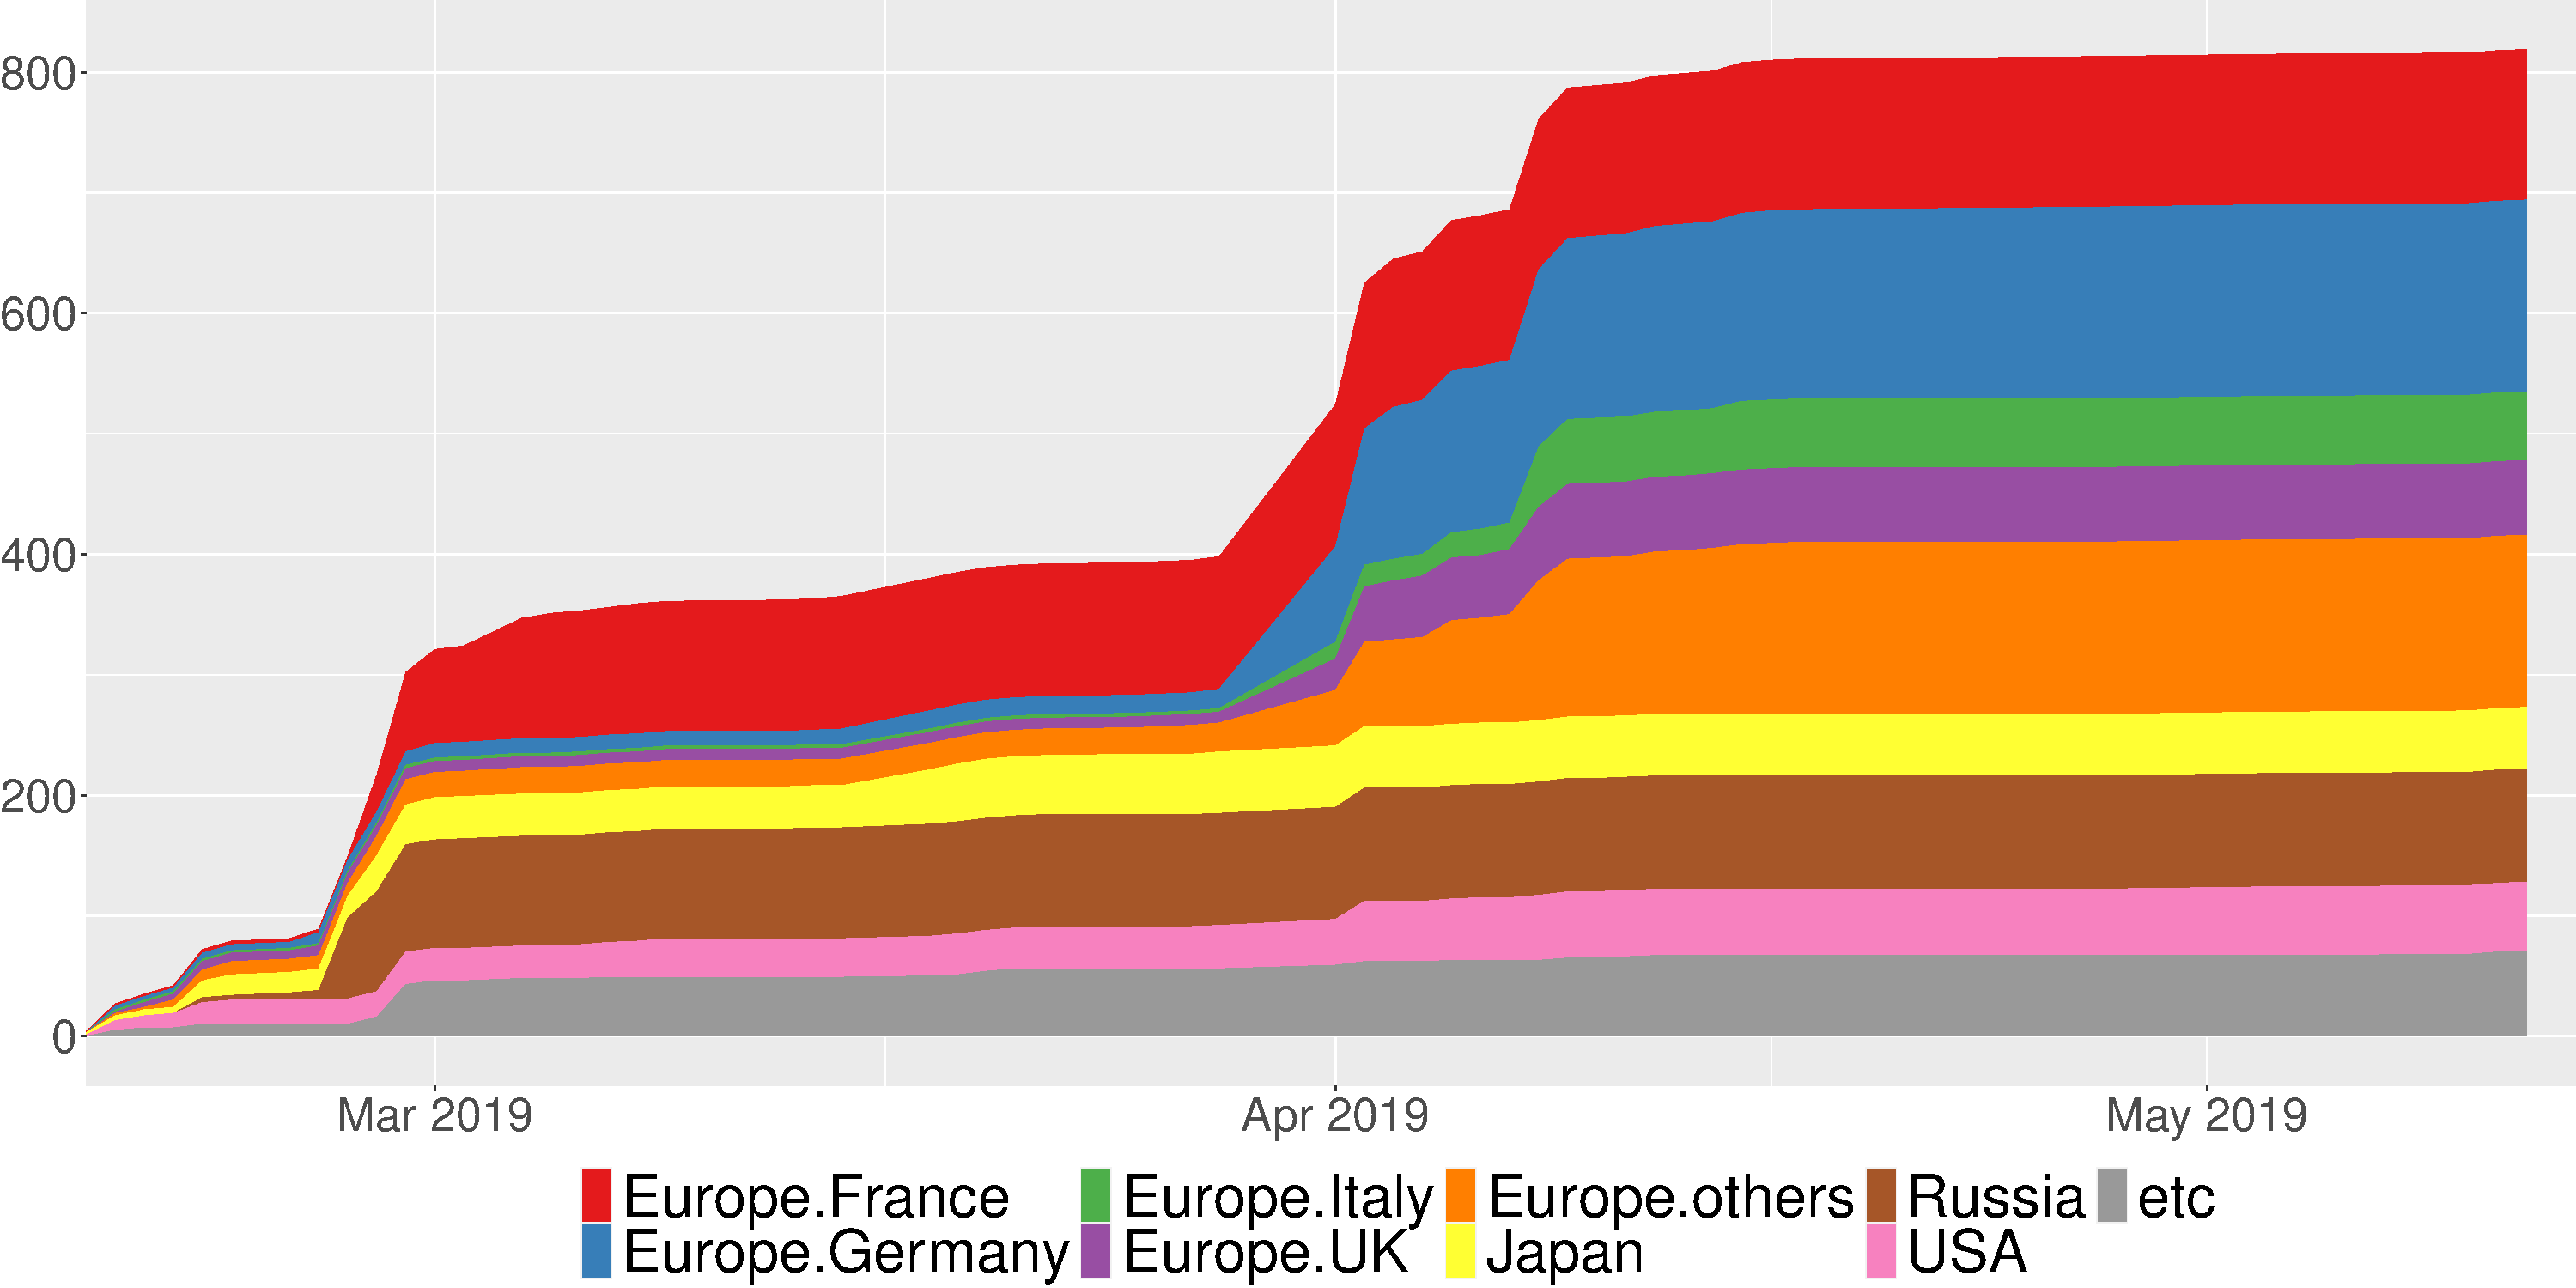
\includegraphics[width=8.0cm]{R-scripts/TimeSeries.pdf}
    \vspace{-2mm}
    \caption{Time series in first 90 days}
    \label{fig:time-series}
  \end{center}
\end{figure}

One of the first questions we had to ask was how to reach a largely
international community of researchers and users, quickly and
efficiently while hoping for a significant contribution.
%
The survey was initially announced via several major mailing lists in the
community such as {\tt hpc-announce@mcs.anl.gov}, but the contributions were
extremely slow to arrive. In order to improve participation, we decided to
approach the problem more locally and reached out to different collaborators and
asked them to locally distribute the questionnaire inside their institutions,
via their own distribution process (mailing list, forums, or different form of
social platforms). As highlighted in Fig.~\ref{fig:time-series}, more localized
means of distribution were highly beneficial, each one of the steps in the
figure corresponding to a new distribution campaign to a new set of
institutions.

% Soon after started, we realized the number of responses was not as many as we
% expected. Hence, we asked people who can reach local regions. Distribution
% using local mailing-lists worked much better than that of major mailing lists.
% Fig.~\ref{fig:time-series} shows the transition of the number of answers at
% the first three months. As shown there are several steps and those steps came
% out after asking local distribution.

This local distribution strategy worked well on some regions but
did not work universally. Table~\ref{tab:countries} shows the number
of participants of top 11 countries (all countries are listed in
\ref{app:countries}).
\revision{Comparing with Table~\ref{tab:top500-share} listing the top 10
countries in the performance share in the Top500~\cite{Top500}, the}{The}
three major countries, USA, China and Japan in Top500, are not even in
the top \revision{5}{four} in our survey. Especially China \revision{has}{had} only 18 participants
including
Taiwan (\revision{2}{two}). We tried to increase the number of participants of those
countries as much as we could, making and distributing \revision{fliers}{flyers} at
several conferences, with little positive outcome. While the root cause is still unclear, this pinpoints to the need for alternative distribution schemes, especially in these locations.
%  Possibly because we could not reach the right influencing person to ask, or
%  maybe because of % nationalities.

\subsection*{\Mcountries}

For the remaining of this report, geographical regions, either countries or
regions, having more than 50 participants, are called {\bf major contributors}
and are the object of cross-tab analysis. Such major contributors are Germany,
France, Russia, UK, Japan, USA, Italy and the rest of European
countries \revision{}{(denoted as ``{\it Europe
    others}''. Table~\ref{app:countries} lists all of them.)}. It
should be noted that the information used to define the \mcountry\ was the
workplaces in the last \revision{5}{five} years and not the nationality of the individual
participants.
%
\revision{}{
The larger number of participants in our survey enables us to conduct
cross-tab analysis between two questions to see if there is a
correlation between the two questions. Doing so on each \mcountry,
then each \mcountry must have enough 
number of answers. The threshold of 50 
participants was selected so that USA and Japan which have the big
performance share in Top500 can be the
\mcountries\ (Table~\ref{tab:countries}, \mcountries\ are in bold
face). It was not our 
intent to define this number as a satisfactory participation
limit. Hence, some cross-tab analysis may not be reliable enough.
However, it should be noted that this cross-tab analysis is possible
because there are larger number of answers than those of precedent
surveys. 
}
%
\begin{table}%
  \small\color{blue}%
\begin{center}%
\caption{Our \Countries\ and Top500 Performance Share}\label{tab:countries}%
\begin{tabular}{c||r|r|r||r|r}%
  \hline%
  &
  \multicolumn{3}{c||}{Top 11 \countries} &
  \multicolumn{2}{c}{Top500} \\
  \Country &
  \multicolumn{3}{c||}{in our survey} &
  \multicolumn{2}{c}{\footnotesize performance share} \\
  \cline{2-6}%
  & Rank & \#Ans & [\%] & Rank & [\%] \\
  \hline%
  \hline%
  {\bf Germany}   & 1 & 159 & 18.7 & 4  & 5.4  \\%
  {\bf France}    & 2 & 125 & 14.7 & 5  & 3.7  \\%
  {\bf Russia}    & 3 & 94  & 11.1 & 18 & 0.4  \\%
  {\bf UK}        & 4 & 67  &  7.9 & 8  & 1.4  \\%
  {\bf Japan}     & 5 & 64  &  7.5 & 2  & 24.4 \\%
  {\bf USA}       & 6 & 58  &  6.8 & 1  & 27.5 \\%
  {\bf Italy}     & 7 & 57  &  6.6 & 6  & 3.2  \\%
  Switzerland     & 8  & 40 &  5.8 & 10 & 1.1  \\%
  South Korea     & 9  & 27 &  3.2 & 13 & 0.8  \\%
  Austria         & 10 & 26 &  3.1 & 27 & 0.1  \\%
  China (+Taiwan) & 11 & 18 &  2.1 & 3  & 23.3 \\%
  \hline%
  \multicolumn{4}{r}{\footnotesize 42 \countries, 851 participants} &
  \multicolumn{2}{c}{\footnotesize (Nov. 2020)} \\%
\end{tabular}%
\end{center}%
\end{table}%

\subsection*{Participants' profile}

Fig.~\ref{fig:occupations} shows the graph of Q1 regarding participants'
occupation. As shown, the majority, roughly 80\% of participants are working at
universities or governmental research institutes. \revision{}{There
  are two type of questions, single-answer and multiple-answer
  questions. This is single-answer question. Hereinafter
  ``{\it (single)}'' or ``{\it (double)}'' is denoted to distinguish them.}
%
\begin{figure}[tb]
  \begin{center}
    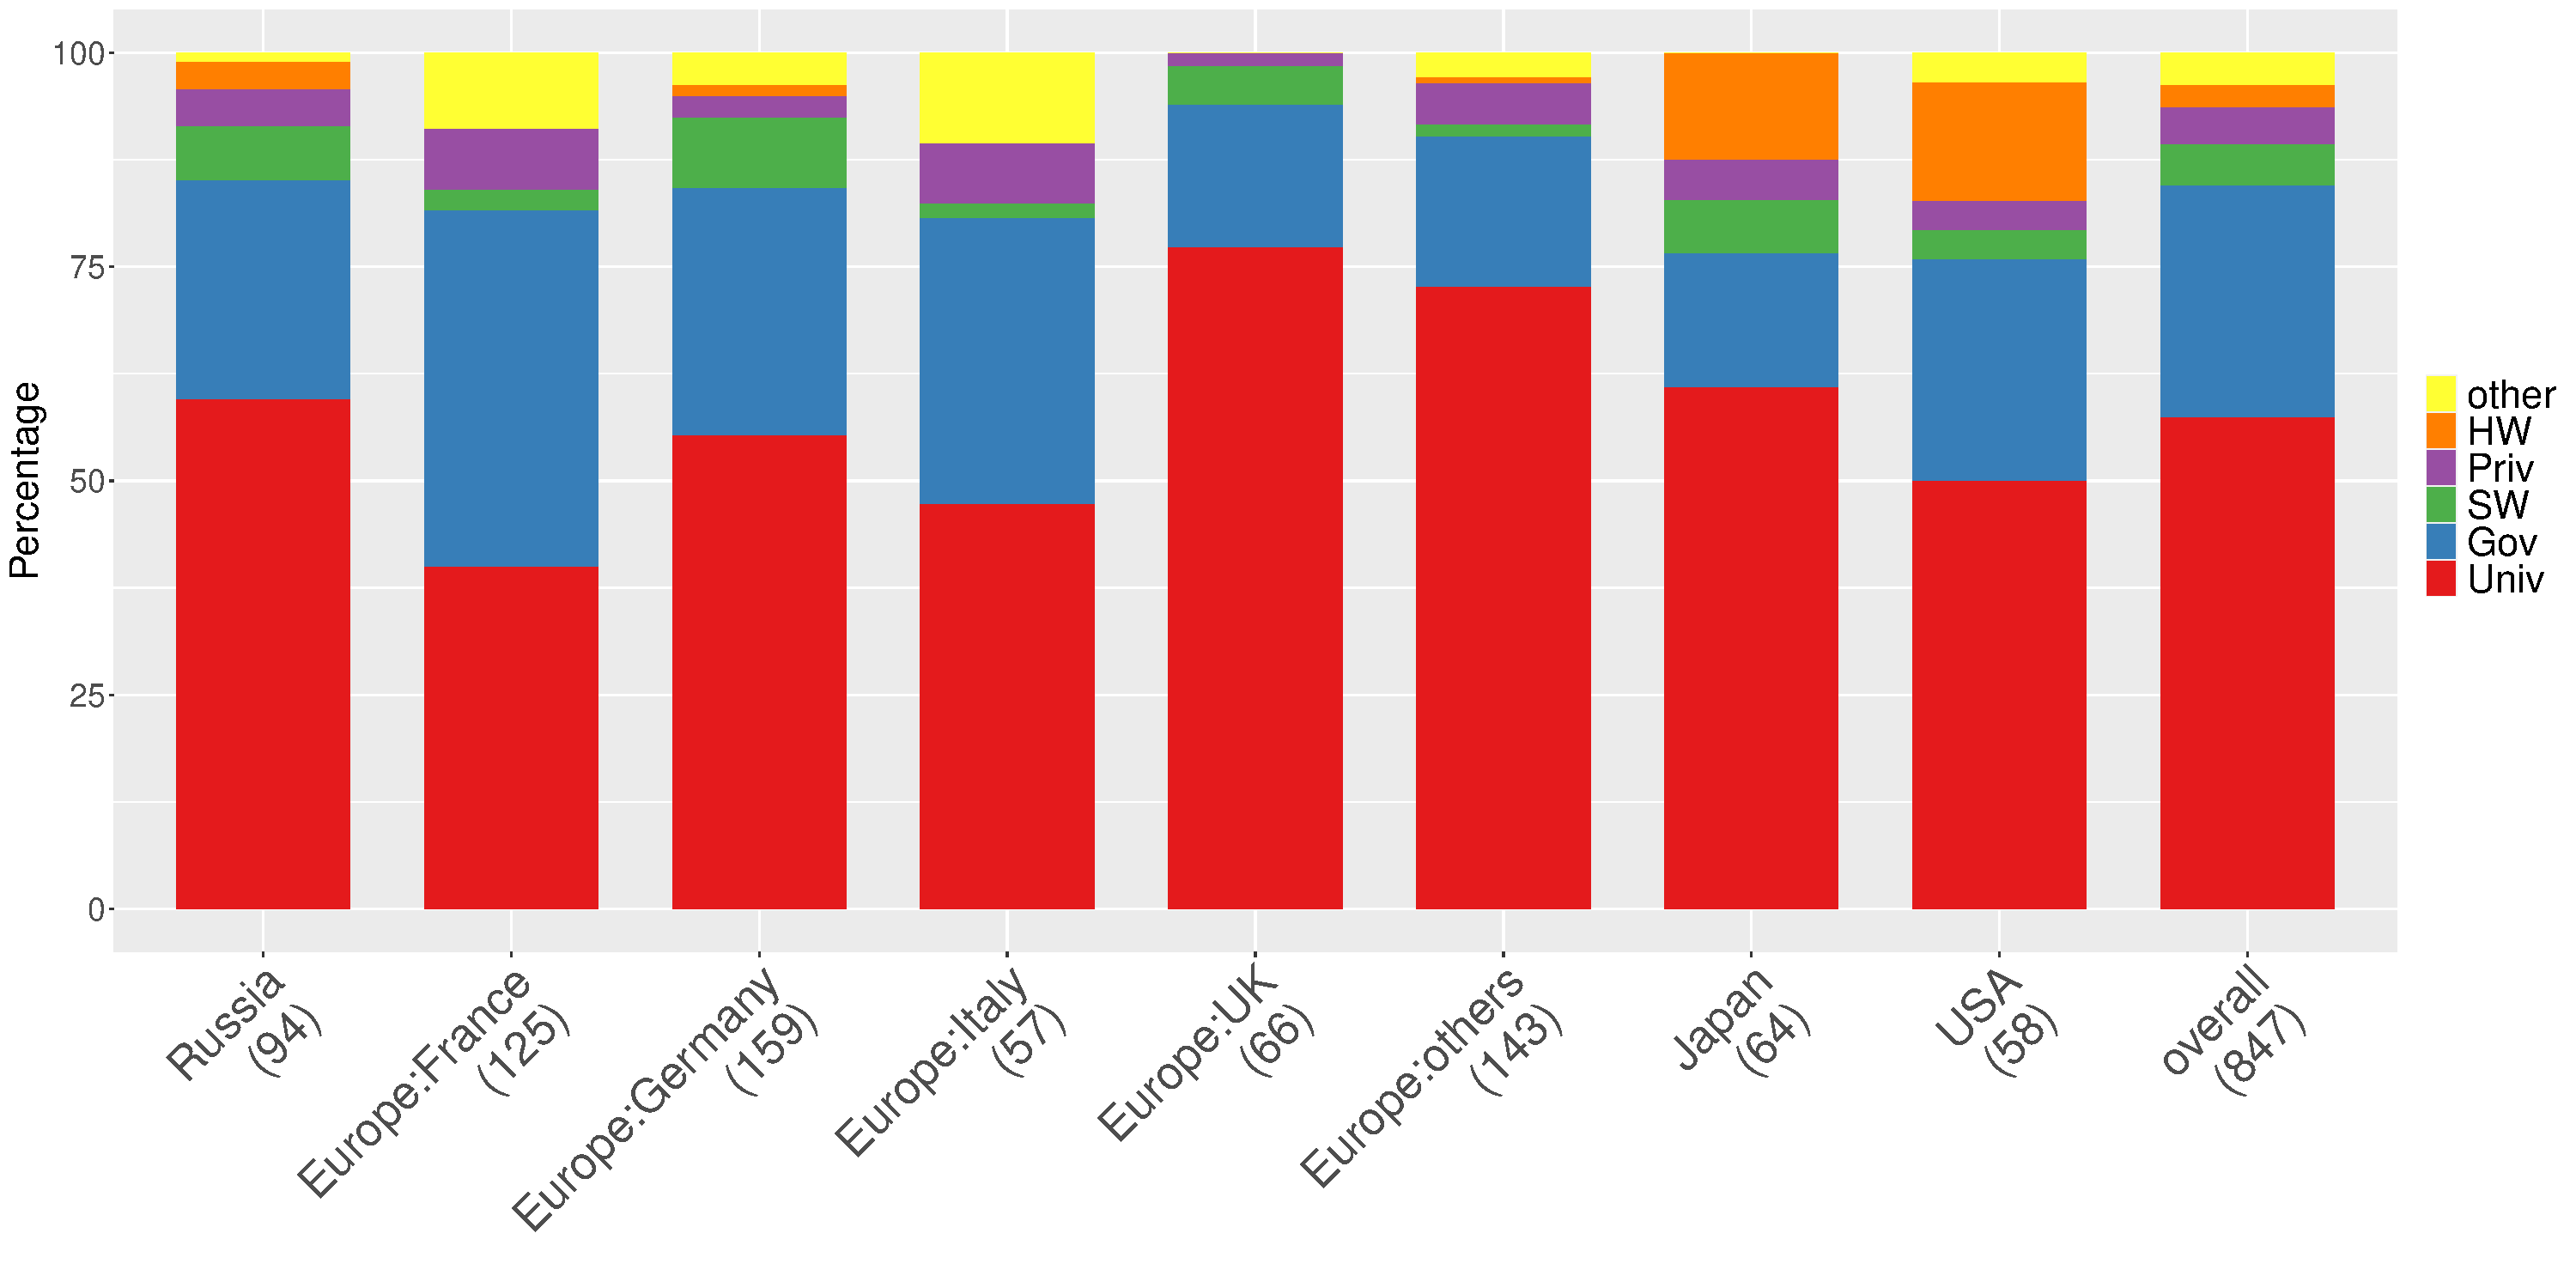
\includegraphics[width=8.0cm]{R-scripts/Q1.pdf}
  \begin{center}
  \end{center}
  \vspace{-10mm}
         {\footnotesize
           \myquote{HW}:Hardware vendor,
           \myquote{Priv}:Private research institute,
           \myquote{SW}:Software vendor, \myquote{Gov}:
           Governmental institute, and \myquote{Univ}:
           College/University)
    }
    \caption{Q1: Occupations {\it(single)}}
    \label{fig:occupations}
  \end{center}
\end{figure}

Fig.~\ref{fig:working-fields} shows the major field the participants are
involved with, field selected among a set of provided choices.
% result of asking \myquote{Which
% fields are you mostly working in?}.
Roughly speaking, most participants are working on numerical applications and/or
libraries, which can either be interpreted as a confirmation that most of the
government sponsored MPI usages are in numerical applications or libraries, or
that it was the most encompassing field among the proposed choices.
%
It is interesting to note that in \revision{2}{two} \mcountries, Japan and US, the percentage of
parallel languages and OS/runtimes participants is significantly higher compared
with the rest of \mcountries.

\begin{figure}[tb]
  \begin{center}
    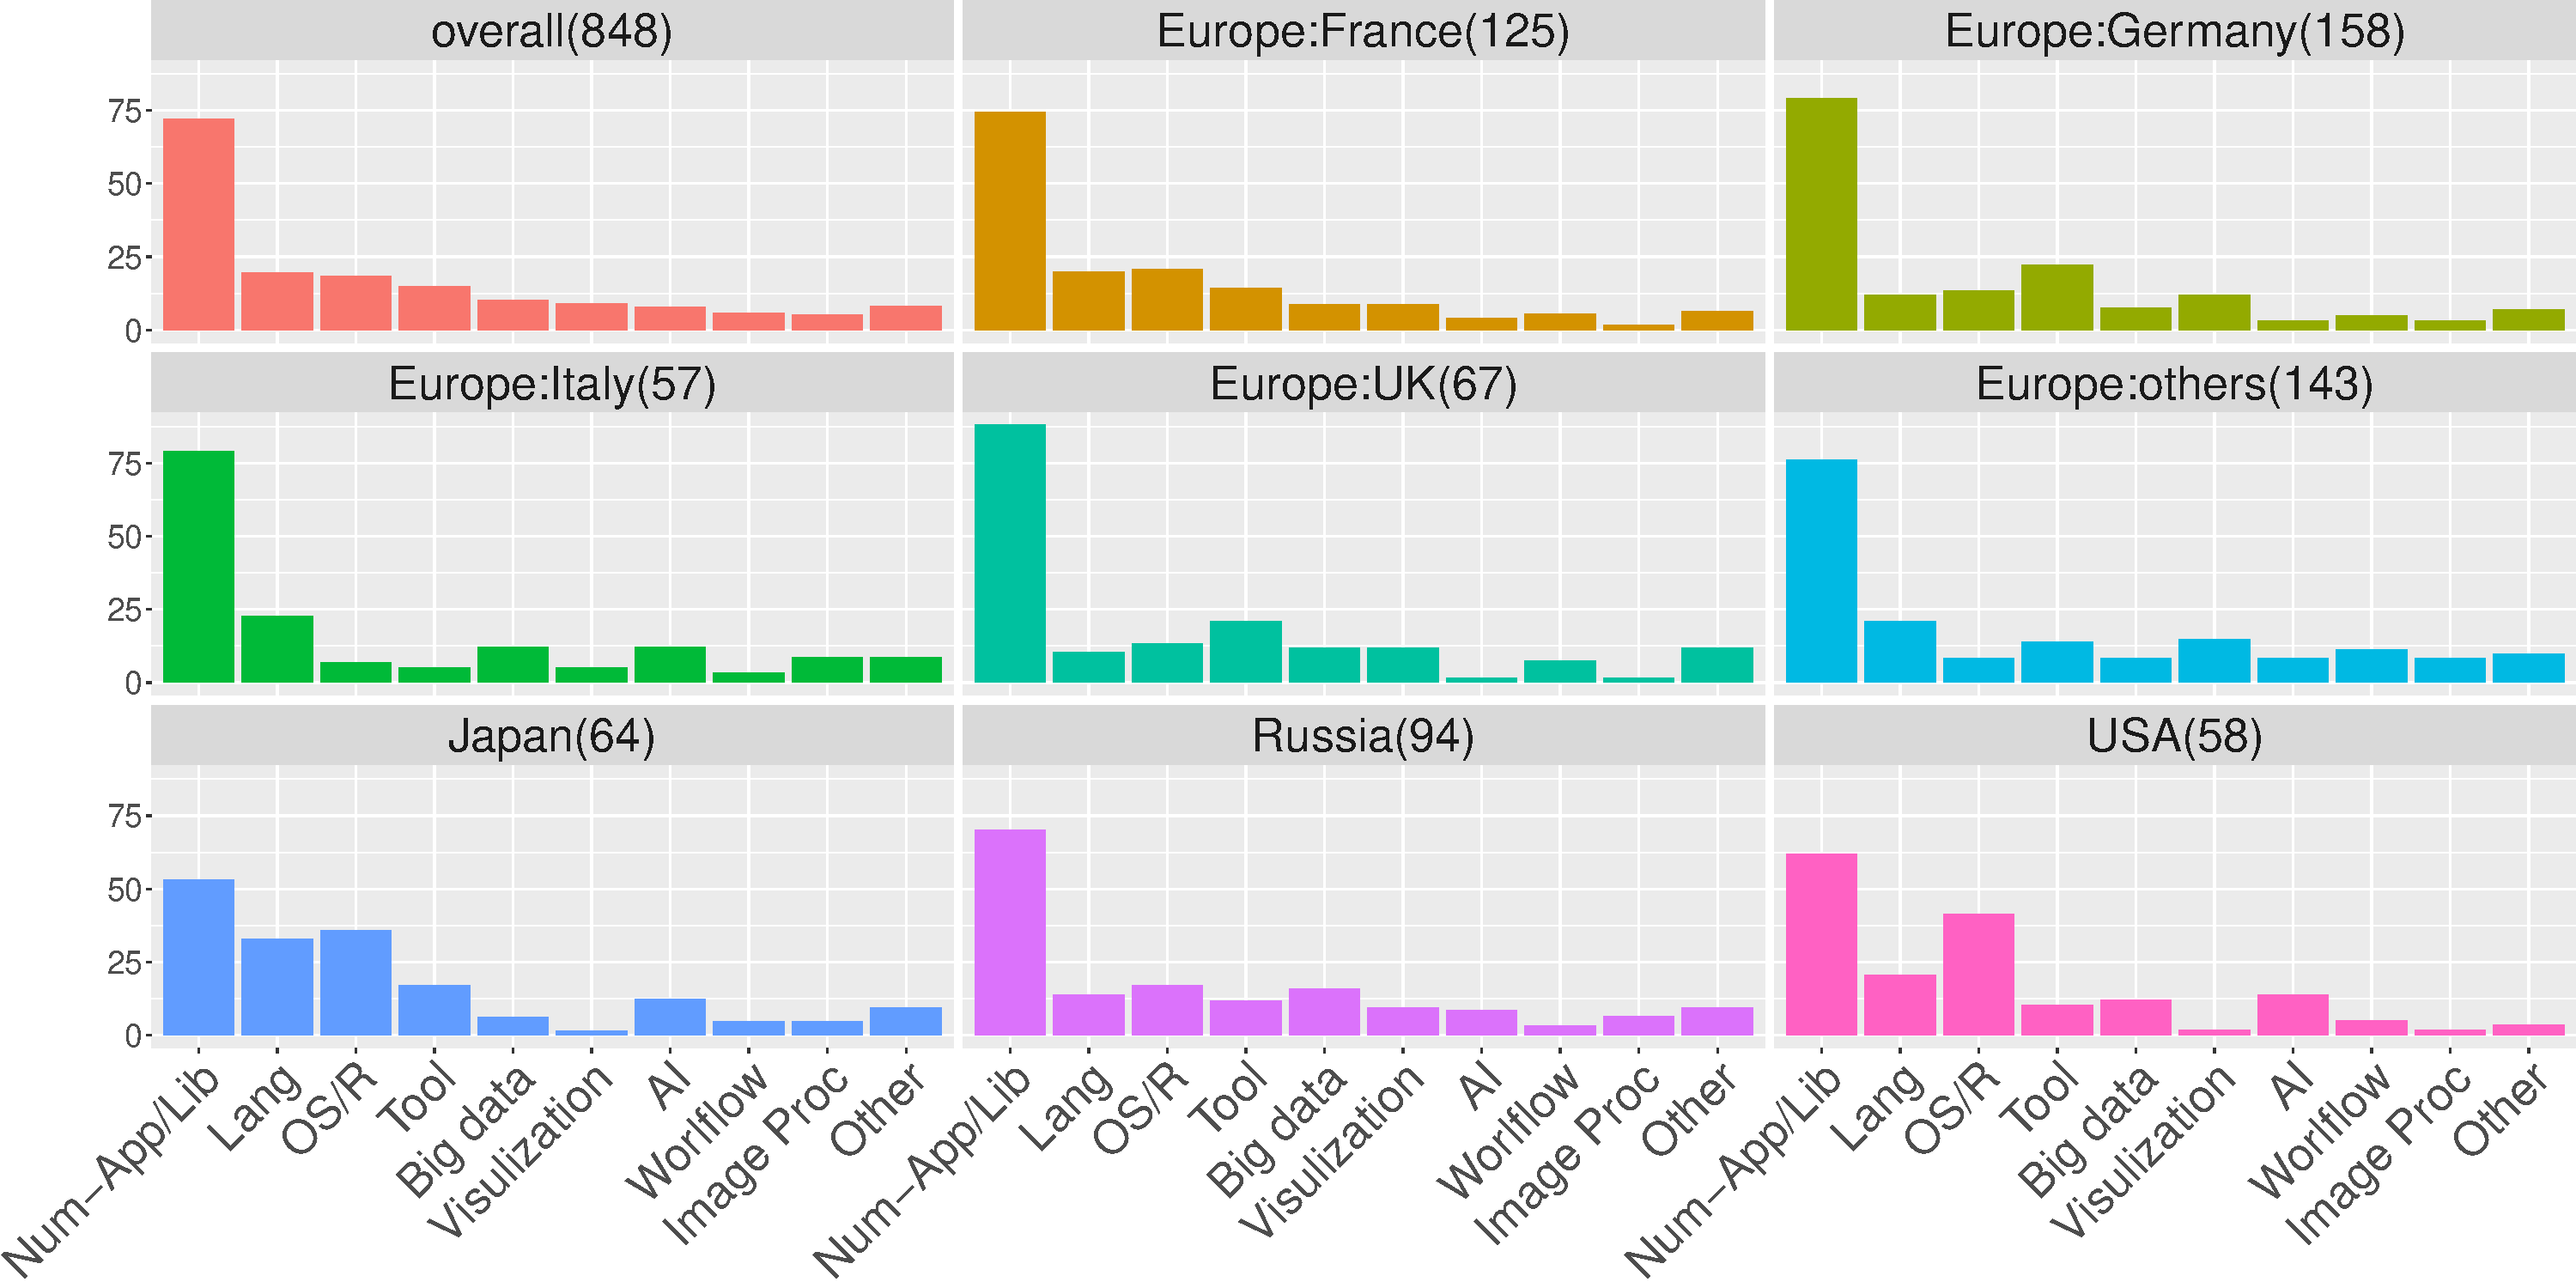
\includegraphics[width=8.0cm]{R-scripts/Q7.pdf}
    \vspace{-2mm}
    \caption{Q7: Working Fields {\it(multiple)}}
    \label{fig:working-fields}
  \end{center}
\end{figure}

\section{Comparison with the ECP survey}\label{sec:ecp}

Although the ECP questionnaire and our questionnaire were designed
independently, there are several comparable
questions. \revision{Before going into the details, we need}{We are
  going} to clarify some points about the profiles of the participants 
in our survey.
%
Due to the target audience reached by the survey propagation means (emails, HPC
related mailing lists, and \revision{community based word-of-the-mouth}{community-based word-of-mouth)}, we can assume
that some of the participants of our survey also participated in the ECP survey.
However, significant differences between the outcome of the two surveys arise.

\begin{figure}[tb]
  \begin{center}
    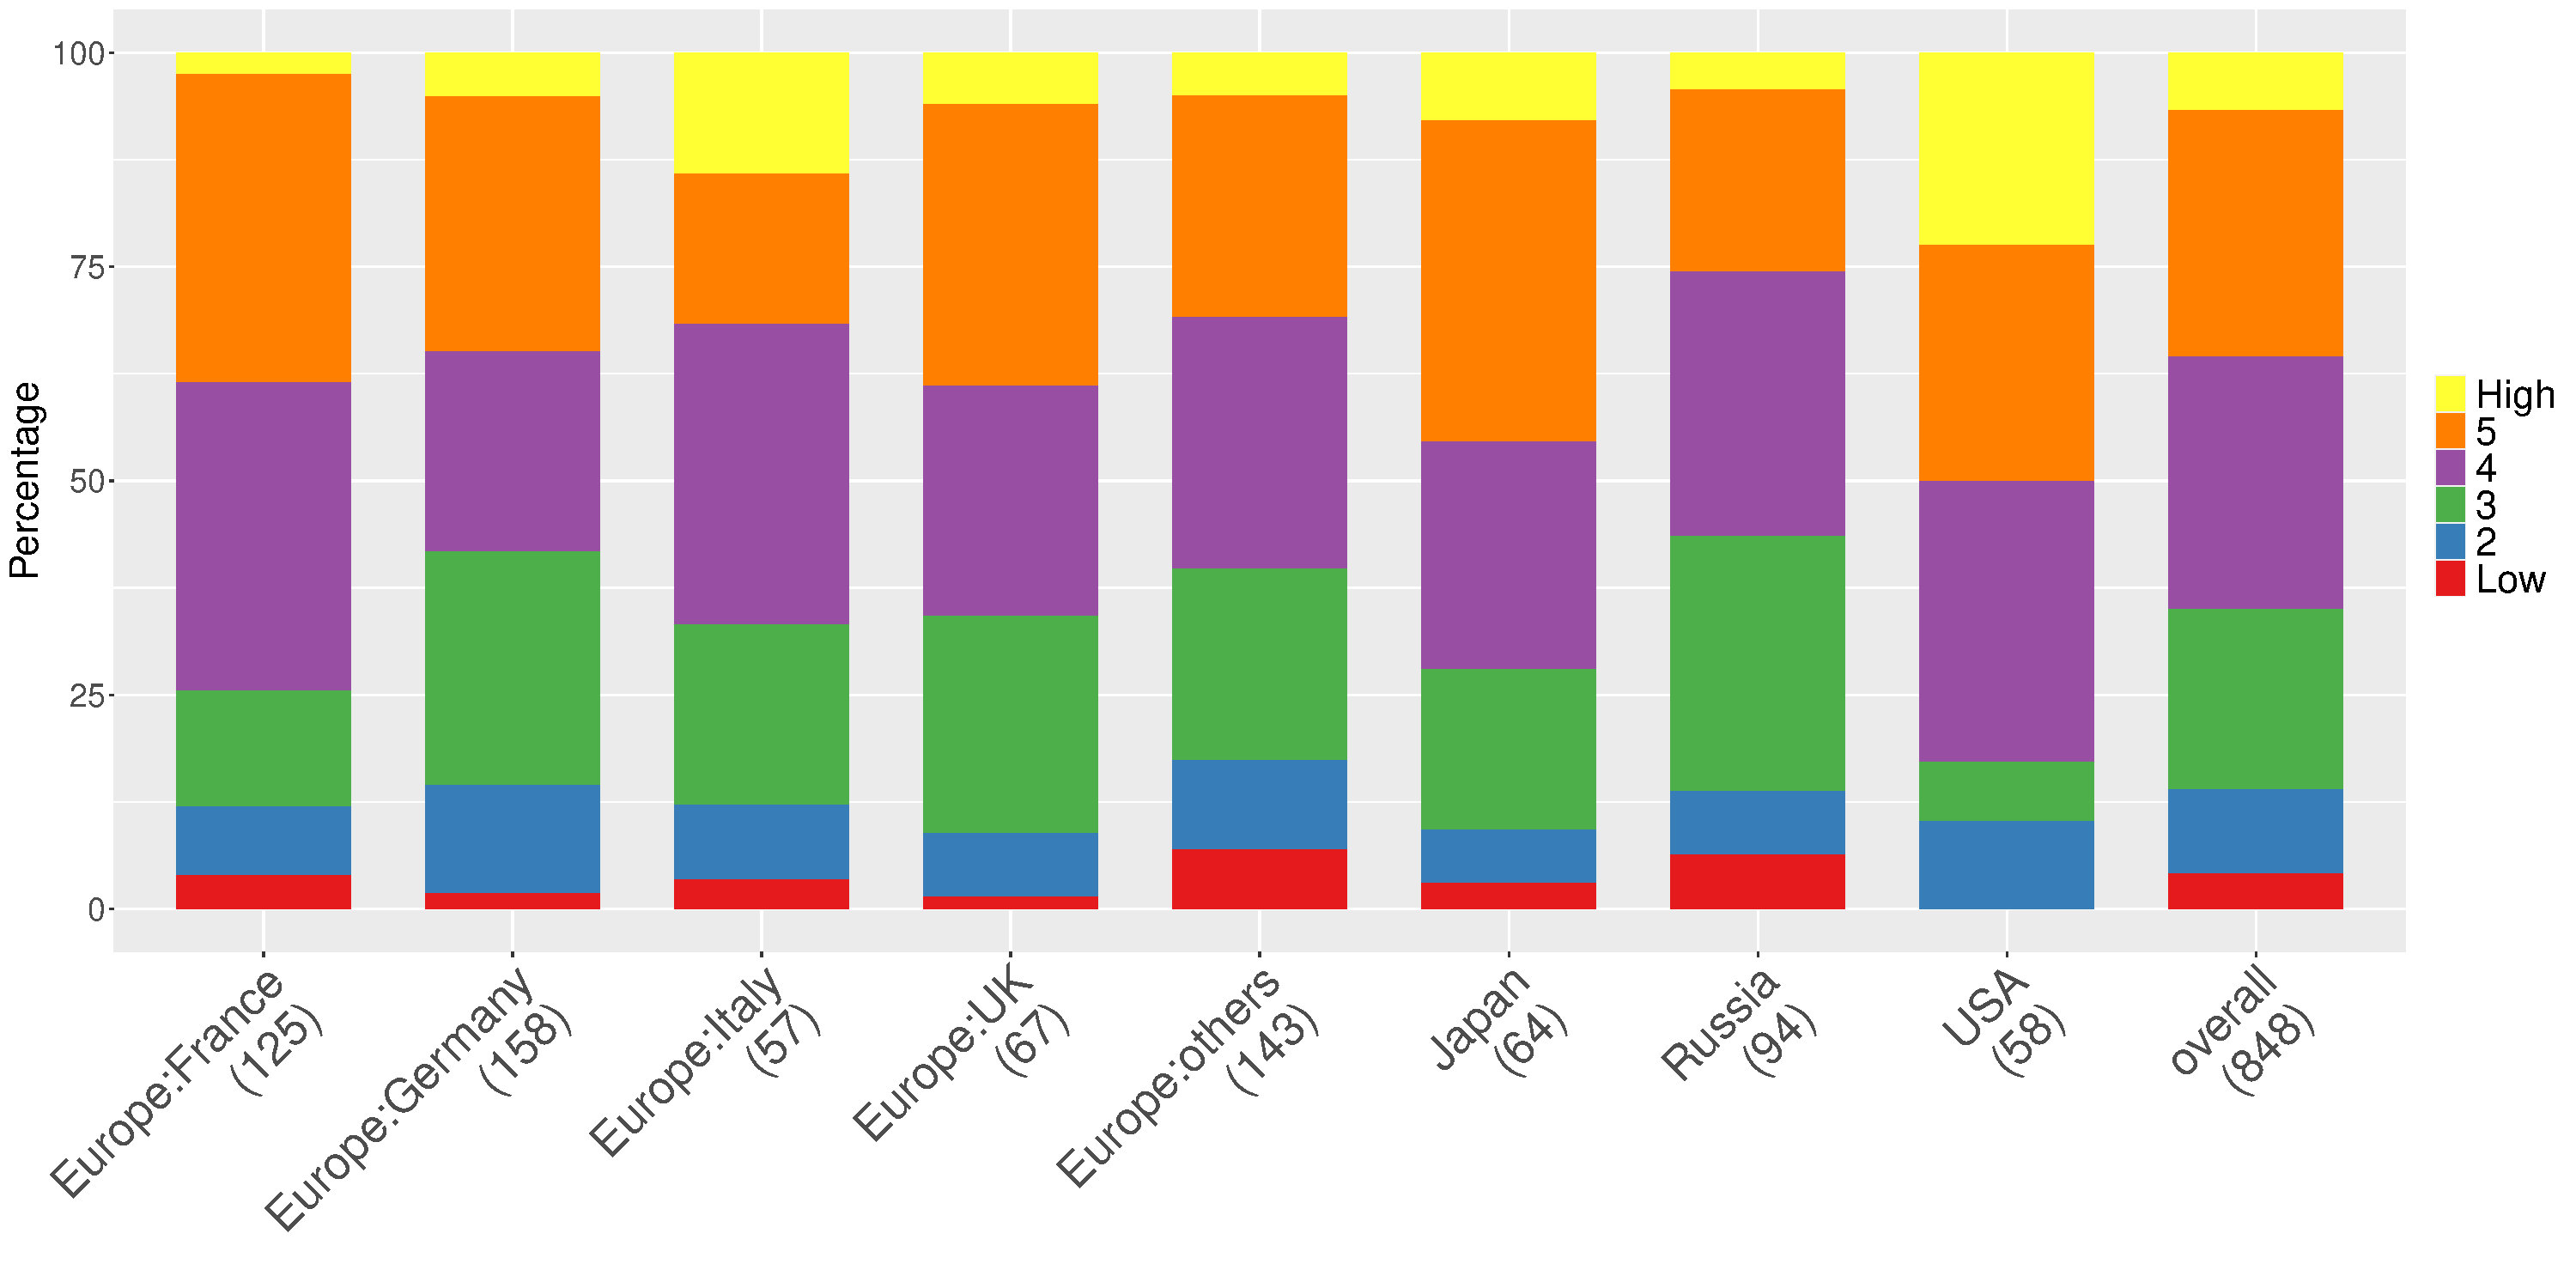
\includegraphics[width=8.0cm]{R-scripts/Q3.pdf}
    \vspace{-2mm}
    \caption{Q3: Self assessment of MPI Skill {\it(single)}}
    \label{fig:mpi-skill}
  \end{center}
\end{figure}

First, and this mainly due to the larger ratio of participants from universities
and national laboratories, it seems likely that the ECP survey contains more
answers from \revision{highly HPC-centered participants or experts MPI
  users}{experts MPI users or highly HPC-centered participants}. 
% We assumed that the participants in the ECP survey have more
% experience on MPI programming than the participants of ours.
Fig.~\ref{fig:mpi-skill} shows the results of \revision{}{the} self-evaluation of the
\revision{participants}{participants'} MPI skill in our survey.  It is worth raising attention to the US
case (right most bar), where almost half of participants rate themselves as
highly skilled MPI users (\myquote{5} or \myquote{High}), significantly ahead
that any other \mcountries. Not only that, but none of the participants
indicated a low MPI-related skill.
% This US percentage in having high MPI skill (\myquote{5} and
% \myquote{High}) is the highest among the other \mcountries\  and nobody in US
% marked the lowest skill.

\begin{figure}[tb]
  \begin{center}
    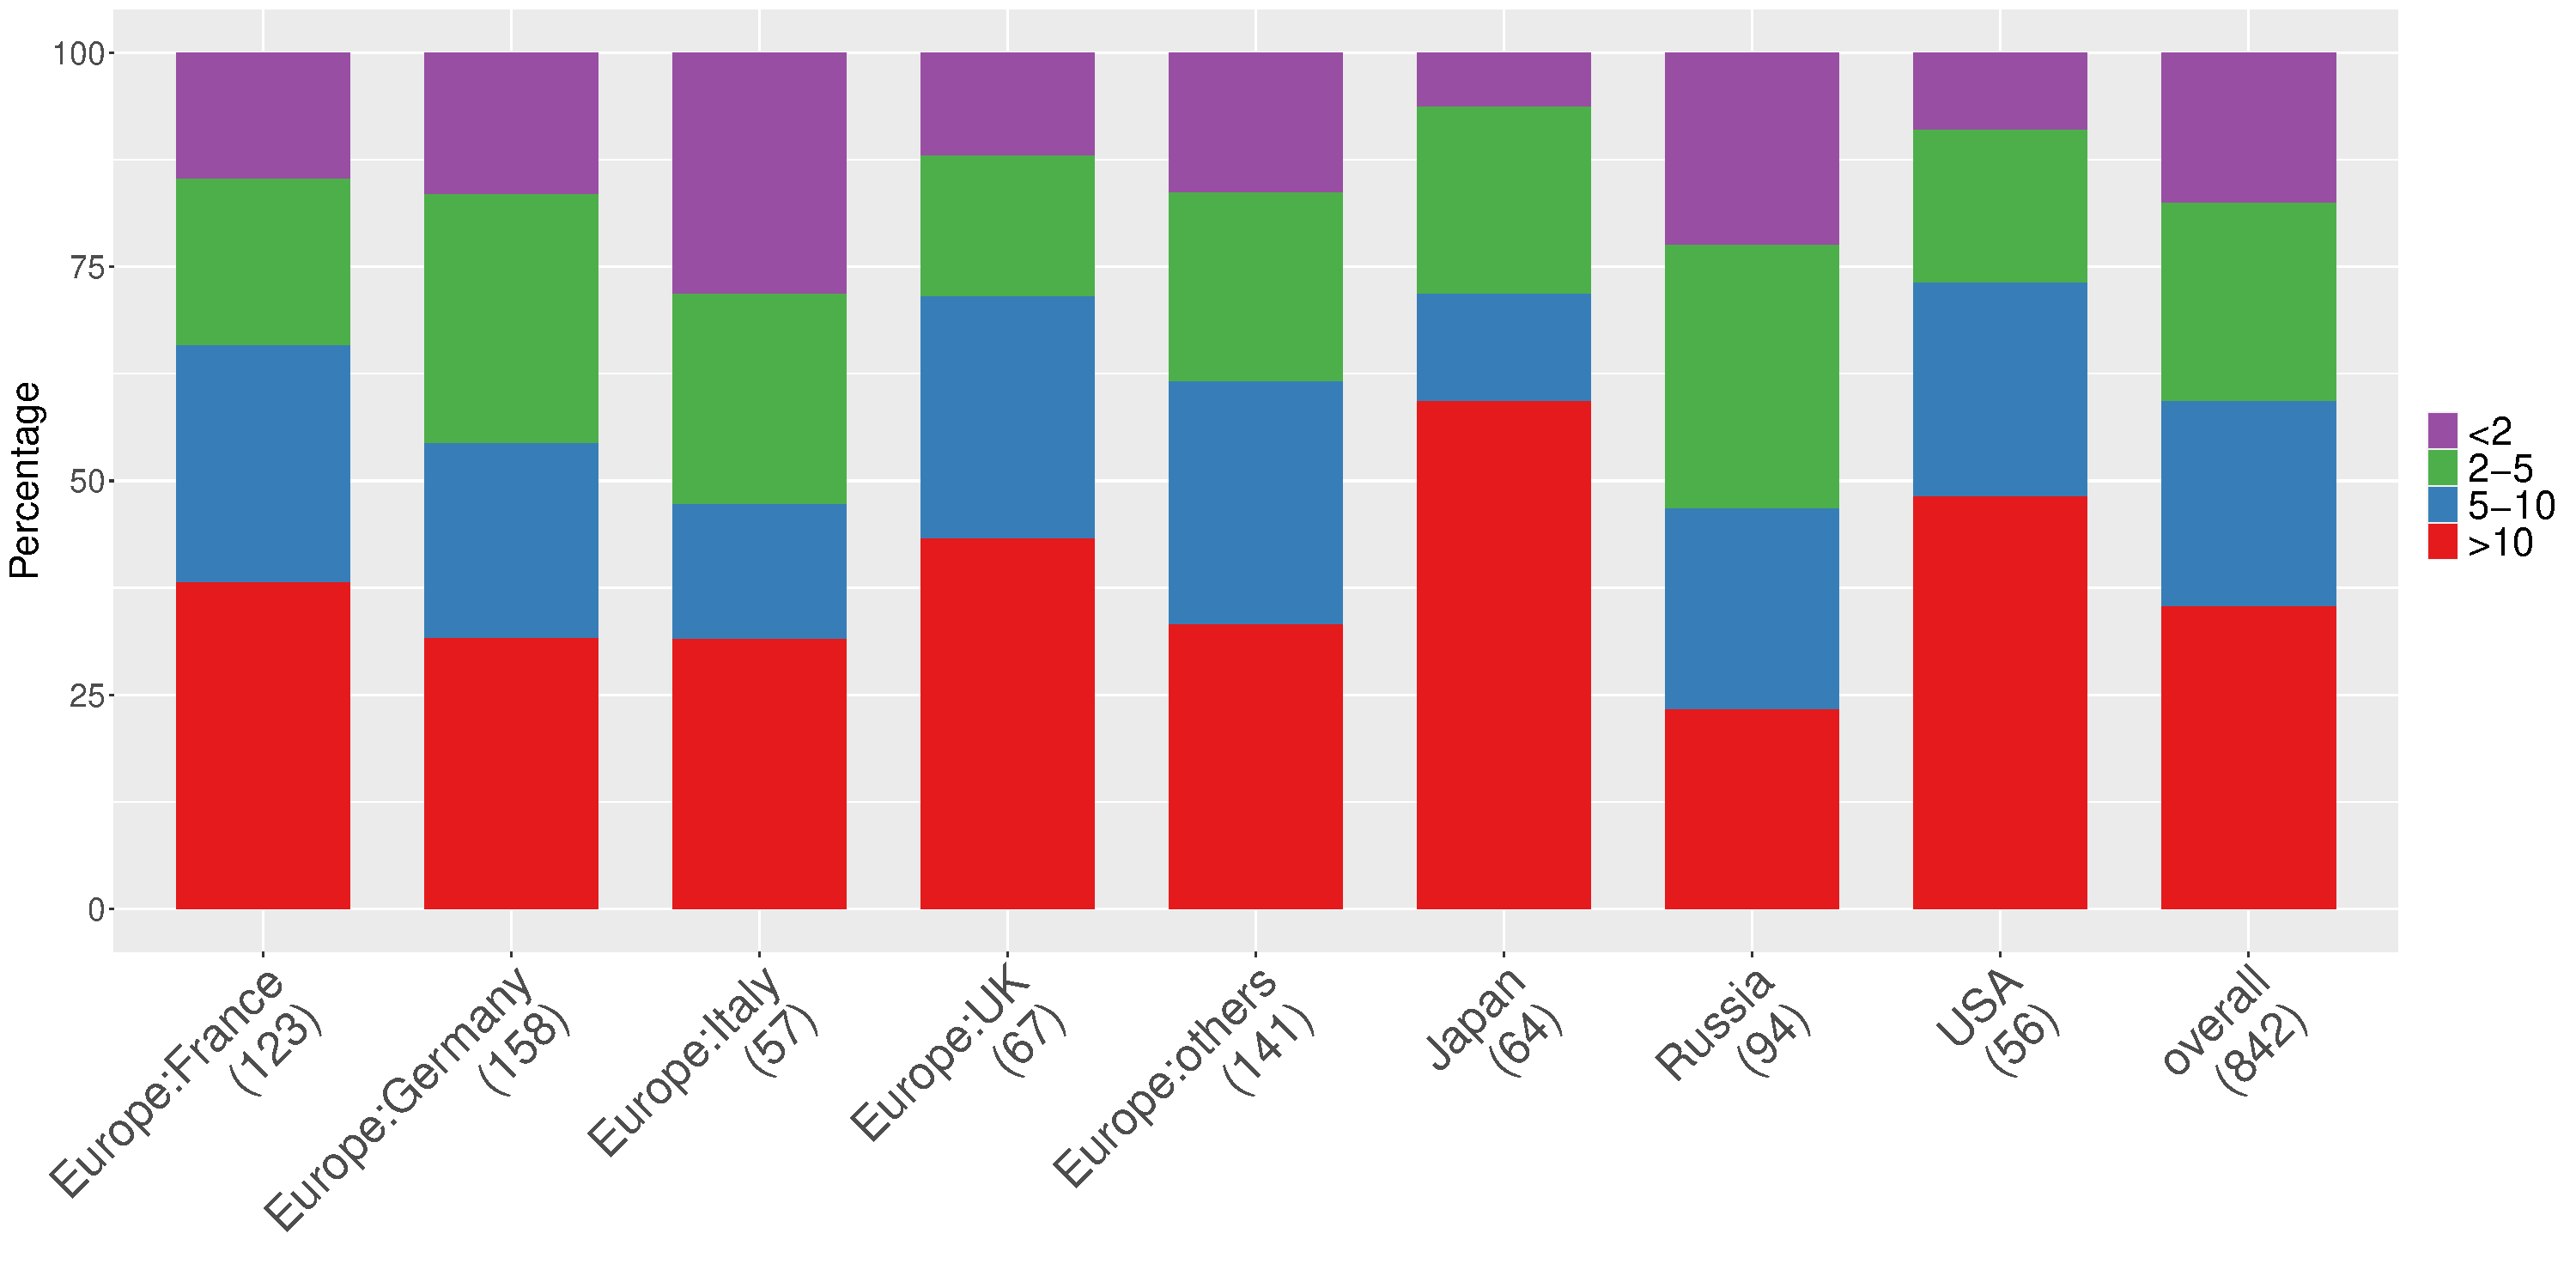
\includegraphics[width=8.0cm]{R-scripts/Q6.pdf}
    \vspace{-2mm}
    \caption{Q6: MPI Experience {\it(single)}}
    \label{fig:mpi-experience}
  \end{center}
\end{figure}

Fig.~\ref{fig:mpi-experience} shows an interesting result, picturing the answers
about participants' expertise via the length of the interactions with the MPI
world. The question was {\it How long have you been writing MPI programs?} and
the choices are {\it more than 10 years} (denoted as \myquote{\textgreater 10}),
\myquote{between 5 and 10 years} (denoted as \myquote{5-10}), \myquote{between 2
and 5 years} (denoted as \myquote{2-5}) and \myquote{less than 2 years} (denoted
as \myquote{\textless 2}). Interestingly only 9\% of US participants have less
than \revision{2}{two} years MPI experience, but they do
\revision{no}{not} rank their MPI expertise the lowest 
(Fig.~\ref {fig:mpi-skill}). Japan followed closely \revision{}{and} has the highest percentage
in participants with more than \revision{10}{ten} years of experience
and also the lowest 
percentage in those with less than \revision{2}{two} years experience. Russia, followed by
Italy, has the highest percentage in less than \revision{5}{five} years experience (including the
less than \revision{2}{two} years experience case).

A second set of questions (Table~\ref{tab:comparable-questions}) with strong
similarities between the ECP and our survey relates to the software stack where
the MPI code is included. We will discuss those results in the following
subsections.

\revision{
\begin{table}[tb]%
  \begin{center}%
    \caption{Comparable Questions}%
    \label{tab:comparable-questions}%
    \begin{tabular}[t]{c|c}
      \hline
      Topic * Our Survey & ECP Survey \\
      \hline
      \hline
      \multicolumn{2}{c}{Layering MPI calls (subsection~\ref{sec:mpi-calls})Layering MPI calls (subsection~\ref{sec:mpi-calls})} \\
      \hline
      \begin{minipage}[t]{0.45\hsize}
        Q21: In most of your programs, do you pack MPI function calls into
        their own file or files to have your own abstraction layer for
        communication?  {\it(single)}
      \end{minipage}
      &
      \begin{minipage}[t]{0.45\hsize}
        Q22: Do you have an abstraction layer that hides the MPI calls? Or do
        most of your developers write MPI calls directly? {\it(single)}
      \end{minipage}
      \\
      \hline
      \hline
      \multicolumn{2}{c}{Using MPI Aspects (subsection~\ref{sec:mpi-aspects})} \\
      \hline
      \begin{minipage}[t]{0.45\hsize}
        Q17: What aspects of the MPI standard do you use in your program in its
        current form? {\it(multiple)}
      \end{minipage}
      &
      \begin{minipage}[t]{0.45\hsize}
        Q35: What aspects of the MPI standard do you use in your application in
        its current form? {\it(multiple)}
      \end{minipage}
      \\
      \hline
      \hline
      \multicolumn{2}{c}{Multi-threading (subsection~\ref{sec:mutil-threading})} \\
      \hline
      \begin{minipage}[t]{0.45\hsize}
        Q18: Which MPI thread support are you using? {\it(multiple)}
      \end{minipage}
      &
      \begin{minipage}[t]{0.45\hsize}
        Q59: Which MPI threading option are you using? {\it(single)}
      \end{minipage}
      \\
      \hline
    \end{tabular}%
  \end{center}%
\end{table}%
}{
\begin{table*}[tb]%
  \begin{center}%
    \caption{Comparable Questions}%
    \label{tab:comparable-questions}%
    \begin{tabular}[t]{c||c|c}
      \hline
      Topic & Our Survey & ECP Survey \\
      \hline
      \hline
      \begin{minipage}[t]{0.13\hsize}
        Layering MPI calls
        (\S~\ref{sec:mpi-calls})
      \end{minipage}
      &
      \begin{minipage}[t]{0.39\hsize}
        Q21: In most of your programs, do you pack MPI function calls into
        their own file or files to have your own abstraction layer for
        communication?  {\it(single)}
      \end{minipage}
      &
      \begin{minipage}[t]{0.39\hsize}
        Q22: Do you have an abstraction layer that hides the MPI calls? Or do
        most of your developers write MPI calls directly? {\it(single)}
      \end{minipage}
      \\
      \hline
      \begin{minipage}[t]{0.13\hsize}
        Using MPI Aspects
        (\S~\ref{sec:mpi-aspects})
      \end{minipage}
      &
      \begin{minipage}[t]{0.39\hsize}
        Q17: What aspects of the MPI standard do you use in your program in its
        current form? {\it(multiple)}
      \end{minipage}
      &
      \begin{minipage}[t]{0.39\hsize}
        Q35: What aspects of the MPI standard do you use in your application in
        its current form? {\it(multiple)}
      \end{minipage}
      \\
      \hline
      \begin{minipage}[t]{0.13\hsize}
        Multi-threading
        (\S~\ref{sec:mutil-threading})
      \end{minipage}
      &
      \begin{minipage}[t]{0.39\hsize}
        Q18: Which MPI thread support are you using? {\it(multiple)}
      \end{minipage}
      &
      \begin{minipage}[t]{0.39\hsize}
        Q59: Which MPI threading option are you using? {\it(single)}
      \end{minipage}
      \\
      \hline
    \end{tabular}%
  \end{center}%
\end{table*}%
}

\subsection{Layering MPI calls}\label{sec:mpi-calls}

\begin{figure}[tb]
  \begin{center}
    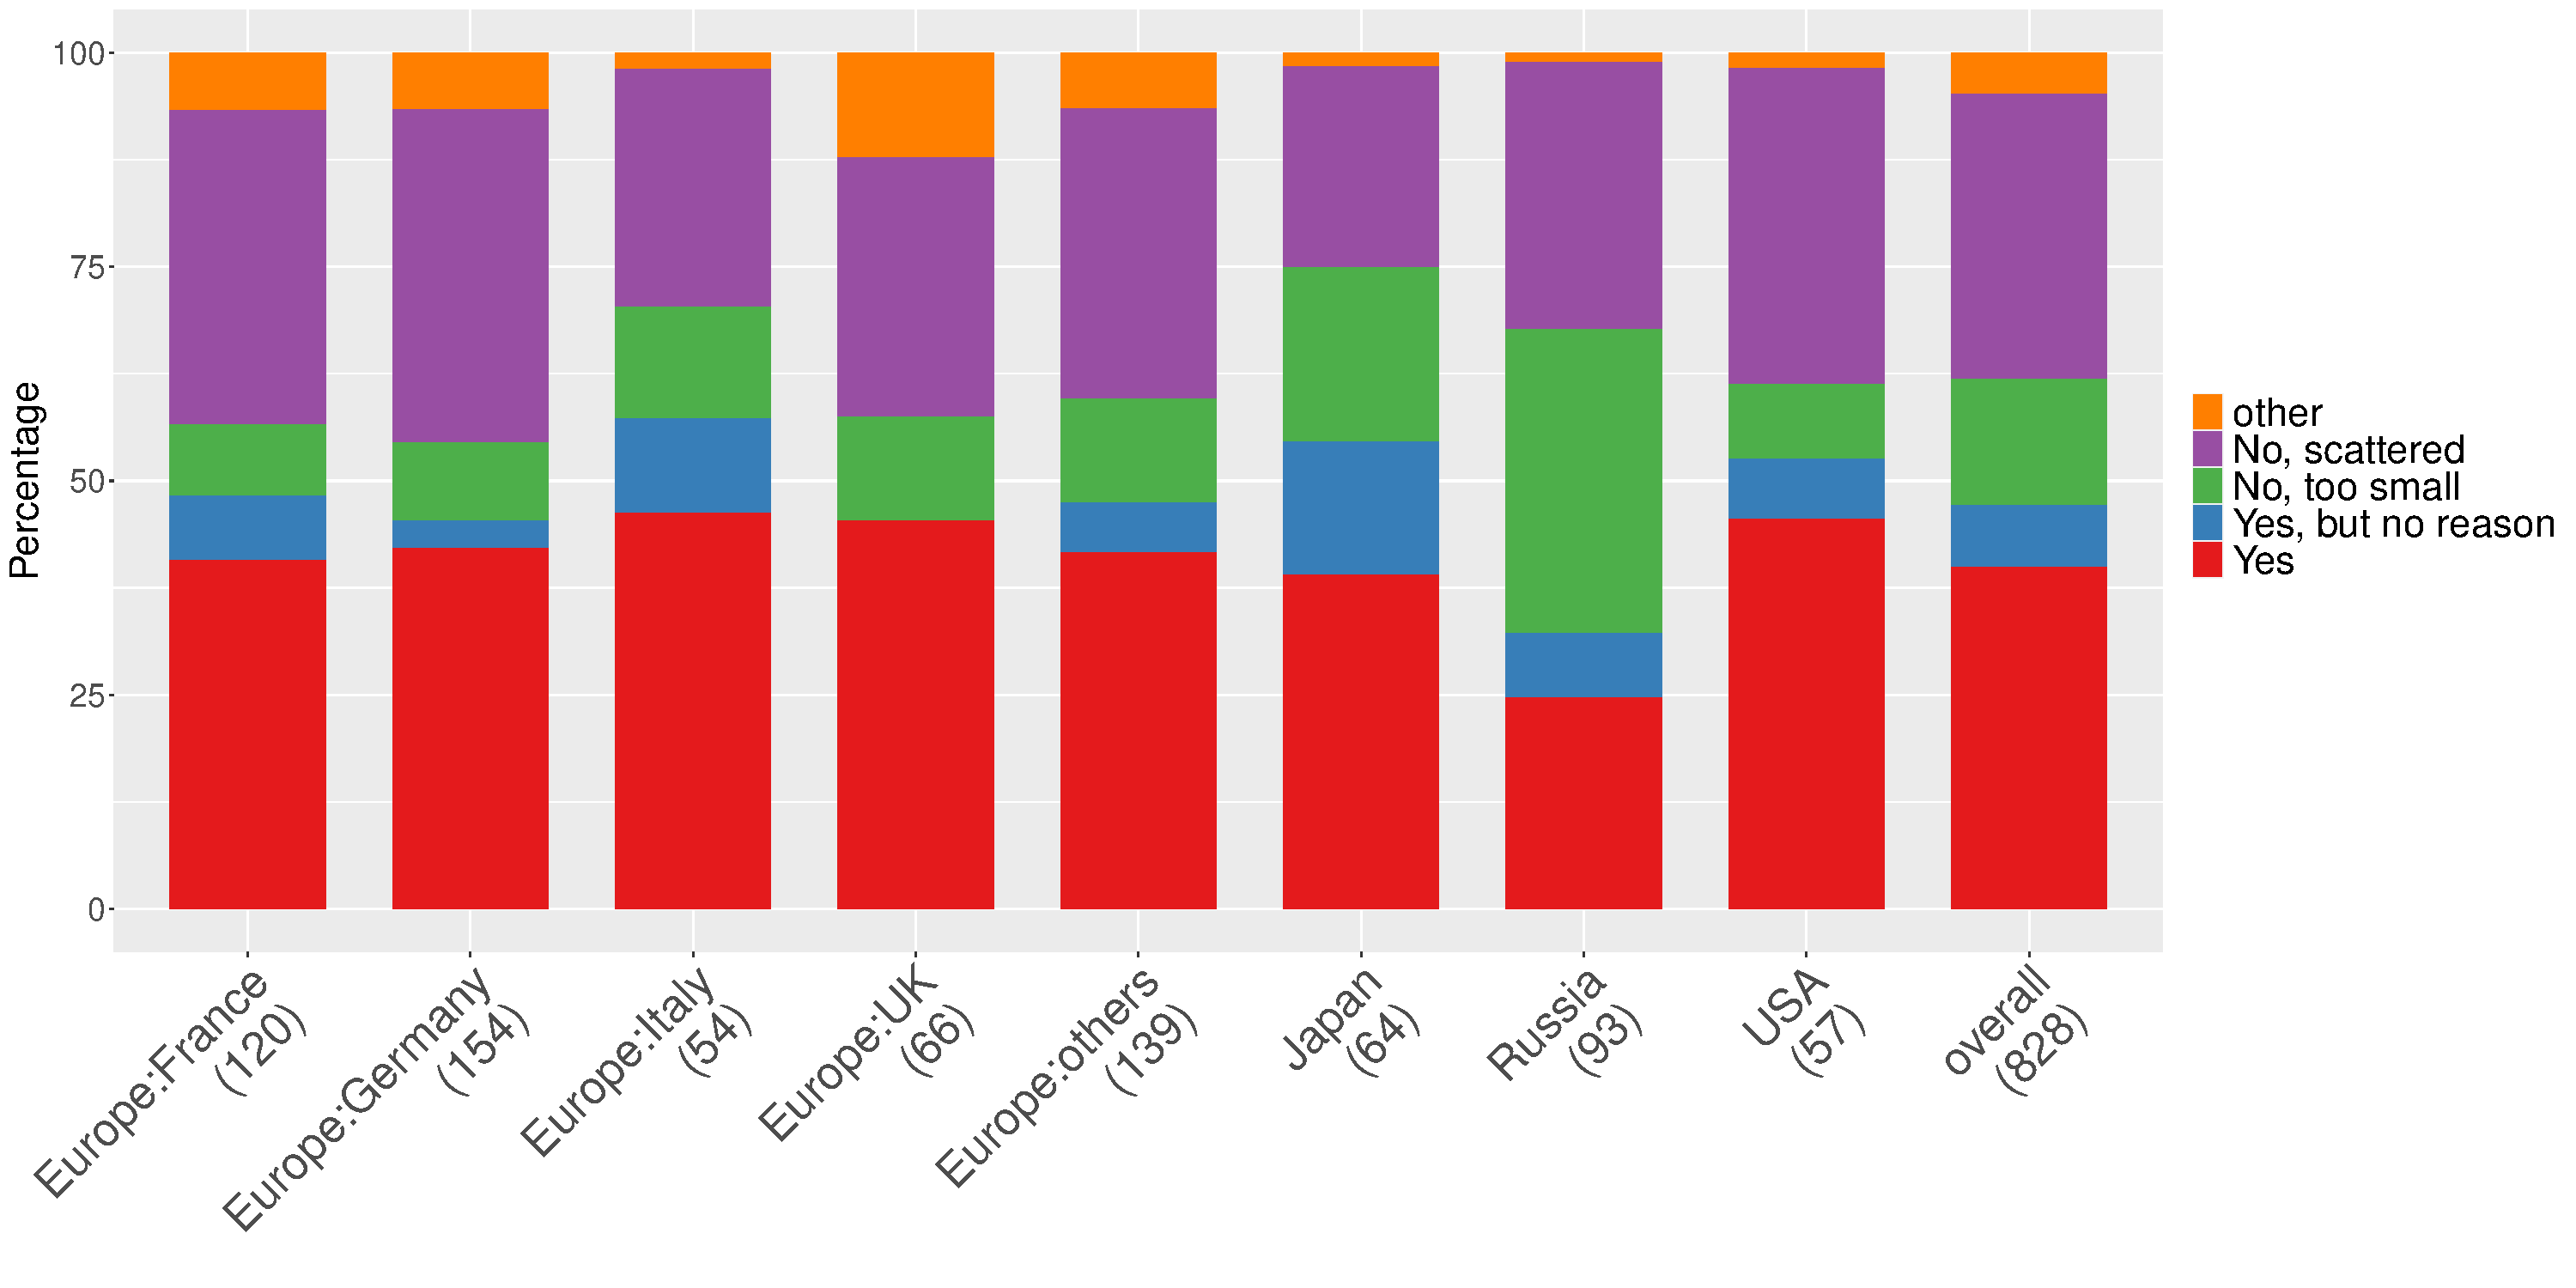
\includegraphics[width=8.0cm]{R-scripts/Q21.pdf}
    \vspace{-2mm}
    \caption{Q21: Layering MPI calls {\it(single)}}
    \label{fig:layering-mpi-calls}
  \end{center}
\end{figure}

Fig.~\ref{fig:layering-mpi-calls} shows the result of our survey and
Table~\ref{tab:layering-mpi-calls} focuses on the comparison between our
and the ECP survey. In the ECP survey, the participants are categorized
into two groups; application development (AD) and system technology
(ST). It is interesting that the percentage of the participants having
MPI layer(s) in our survey is roughly 50\% even in the US, whilst the
ratio of yes and no is approximately $6:4$ in the ECP survey.
Having a closer look at Fig.~\ref{fig:layering-mpi-calls}, the answer,
\myquote{No, my program is too small to do that}, dominates in Russia. In
the other \mcountries, the participants having a packing layer occupies
40-50\%.

\begin{table}[tb]%
  \small%
  \begin{center}%
    \caption{Layering MPI calls}\label{tab:layering-mpi-calls}%
    \begin{tabular}{c|c||c|c||c|c|c}%
      \hline%
      \multicolumn{2}{c||}{Choice} & \multicolumn{2}{c||}{Our Survey [\%]} &
      \multicolumn{3}{c}{ECP [\%]} \\
      \cline{3-7}%
      \multicolumn{2}{c||}{} & overall & USA & AD & ST & AD+ST \\
      \hline%
      \hline%
      Yes & - & 40 & 46 & & & \\
      & no reason & 7 & 7 & & & \\
      \cline{2-4}%
      & (sum) & 47 & 53 &  79 & 46 & 62 \\
      \hline%
      \hline%
      No & too small & 15 & 9 & & & \\
      & - & 33 & 37 & & & \\
      \cline{2-4}%
      & (sum) & 48 & 46 & 21 & 54 & 38 \\
      \hline%
      \hline%
      Other & - & 5 & 2 & - & - & - \\
      \hline%
    \end{tabular}%
  \end{center}%
\end{table}%

\subsection{Using MPI Features}\label{sec:mpi-aspects}

The Q35 in the ECP survey and Q17 in our survey are equivalent
questions, although the answer choices are somewhat
different. Fig.~\ref{fig:using-mpi-aspects} shows the result of our
survey and Fig.~\ref{fig:using-mpi-aspects-comp} shows the comparison
between ECP's and ours on the same choices. As shown in
Fig.\ref{fig:using-mpi-aspects}, the
using aspects can be categorized in three groups; A) more frequently
used (point-to-point and collectives), B) second frequently used
(\myquote{Datatypes}, \myquote{with OpenMP}, \myquote{Communicator}, and \myquote{One-sided}), and C) less
frequently used (\myquote{PMPI}, \myquote{Persistent}, and
\myquote{dyn. process} (dynamic process).
%
It should be noted that all these less frequently used features were already
introduced and standardized in MPI 2.2 which was \revision{release}{released} in 2009. This is
clearly a concerning factor for the popularity of some of the MPI features as
despite the 10-year existence many of the features failed to get any traction
outside a small, certainly dedicated crowd.

\begin{figure}[tb]
  \begin{center}
    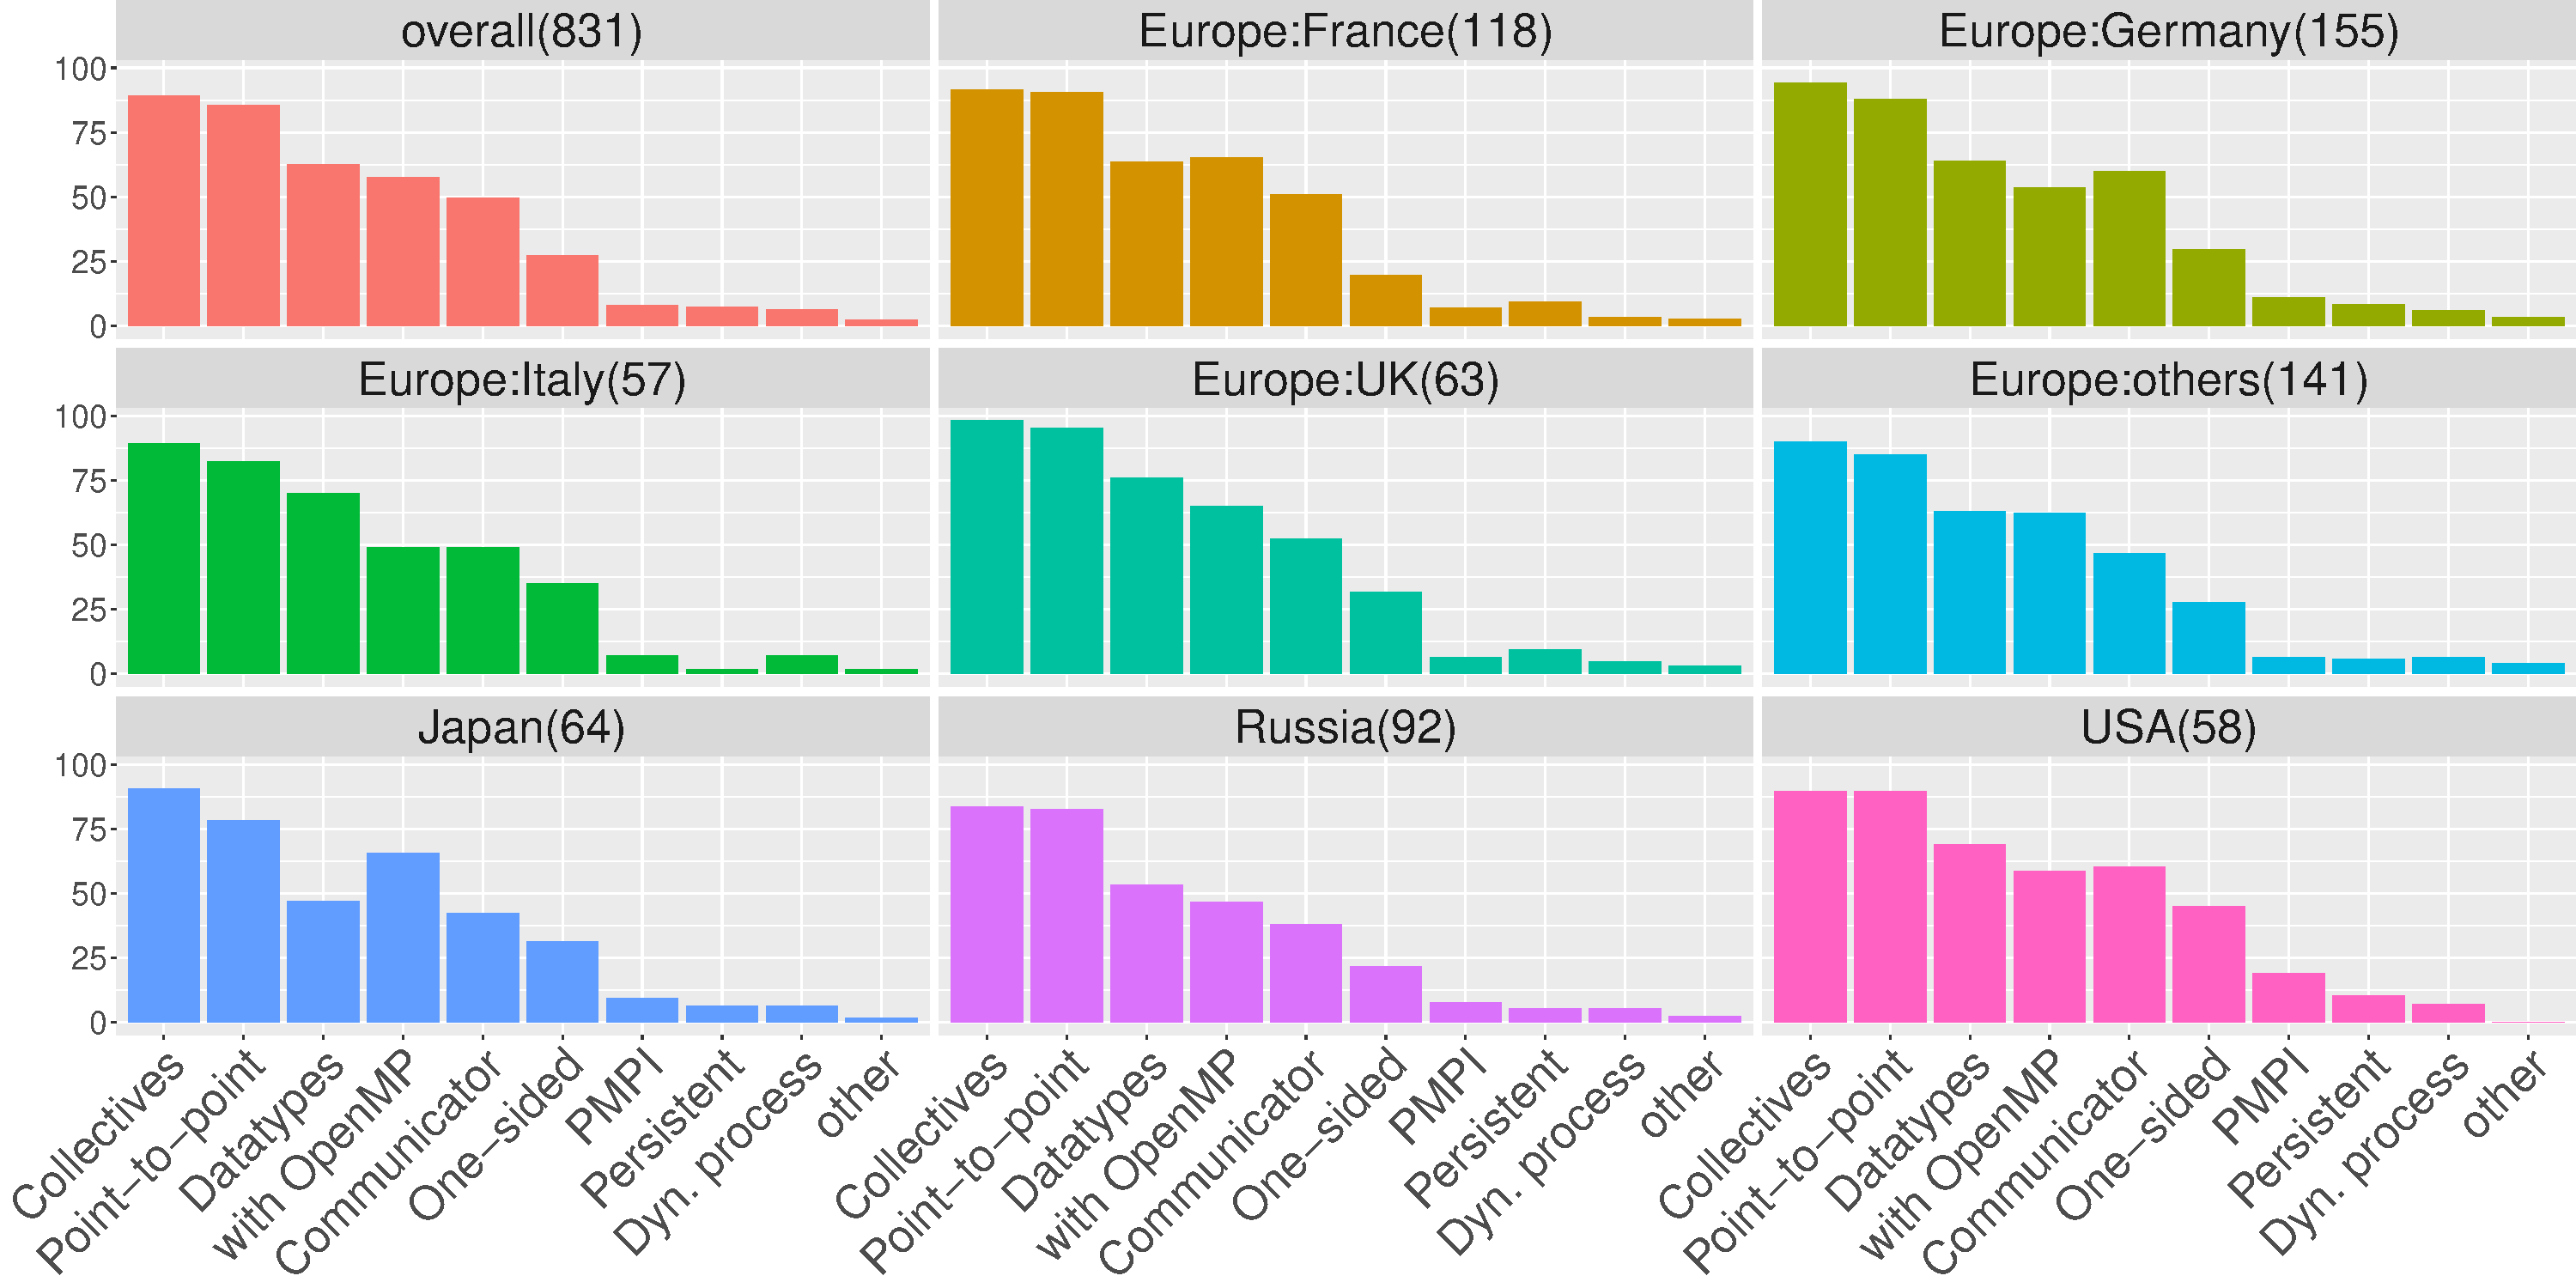
\includegraphics[width=8.0cm]{R-scripts/Q17.pdf}
    \vspace{-2mm}
    \caption{Q17: Using MPI Aspects {\it(multiple)}}
    \label{fig:using-mpi-aspects}
  \end{center}
\end{figure}

The most notable difference between the two surveys relates to the use of
datatypes (Table~\ref{fig:using-mpi-aspects-comp}). The percentage of datatype usage
in the ECP was around 23\% while in our survey it is significantly higher, at
more than 60\% in both overall and USA contributors.
%
Looking at the USA data, as it is difficult to imagine that the common
participants changed their mind between the two surveys, it seems that the
datatype usage is more developed outside national laboratories. But at this
point this conclusion is conjectural, more thorough analysis is needed to gain a
better understanding.
% In the ECP survey, there are three questions asking using MPI aspects in
% different usage scenarios; \begin{enumerate*} \item current, \item exascale, and
% \item performance critical \end{enumerate*}. In all three questions, the
% percentages of using datatype are low.

\revision{
\begin{table}[tb]%
  \begin{center}%
    \caption{Using MPI Aspects}\label{tab:using-mpi-aspects}%
    \begin{tabular}{c||c|c||c|c|c}%
      \hline%
      Choice & \multicolumn{2}{c||}{Ours [\%]} &
      \multicolumn{3}{c}{ECP {\scriptsize (current usage)} [\%]} \\
      \cline{2-6}%
      & overall & USA & AD & ST & {\small AD+ST} \\
      \hline%
      Collectives & 89 & 90 & 86 & 75 & 80 \\
      Point-to-point & 85 & 90 & 96 & 79 & 88 \\
      Datatype & 63 & 69 & 25 & 21 & 23 \\
      Communicator & 50 & 60 & 68 & 54 & 61 \\
      {\small One-sided (RMA)} & 27 & 45 & 36 & 7 & 21 \\
      PMPI & 8 & 19 & 11 & 0 & 14 \\
      \hline%
      \multicolumn{6}{r}{\small * Both are multiple answer questions} \\
      \multicolumn{6}{r}{\small ** Common choices in both surveys are shown}\\
    \end{tabular}%
  \end{center}%
\end{table}%
}
{

\begin{figure}[tb]
  \begin{center}
    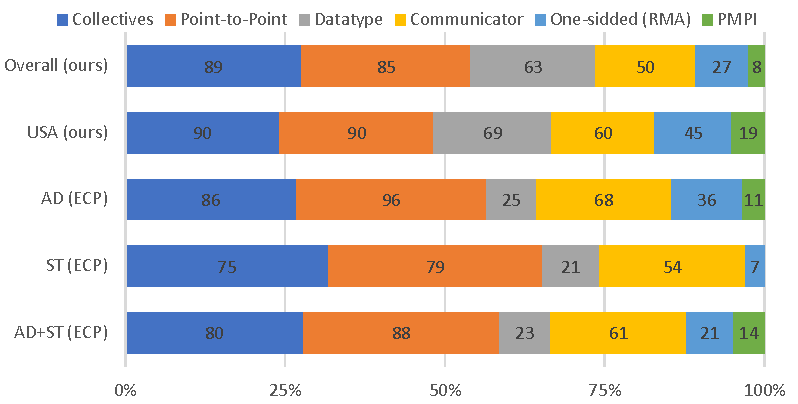
\includegraphics[width=8.0cm]{Figs/MPI-Aspects.pdf}
    \vspace{-2mm}
    \caption{Using MPI Aspects}\label{fig:using-mpi-aspects-comp}%
  \end{center}
\end{figure}
}

Fig.~\ref{fig:skill-and-aspects} is a heatmap representing the cross-tab
analysis between participants' MPI skills (Q3) and the knowledge or use of MPI
features (Q16). The darker the color of a cell, the higher the frequency (Legend
combined with color bar can be found at the bottom of the figure. The numbers in
the legend cells are percentages). Less frequent rows (\revision{1}{one} is the lowest skill and
\revision{6}{six} is the highest skill) in this figure are omitted to increase readability. The
result is interesting in the sense it \revision{goes against}{contradicts} the expected outcome, where
MPI experts will know and use more features. What we observe here is that the
less used features in Fig.~\ref{fig:using-mpi-aspects}, PMPI, persistent, and
dynamic process, are almost independent from the MPI skill.

% Natural thinking may conclude that the higher the MPI skill, lesser the unknown
% MPI features.

\begin{figure}[tb]
  \begin{center}
    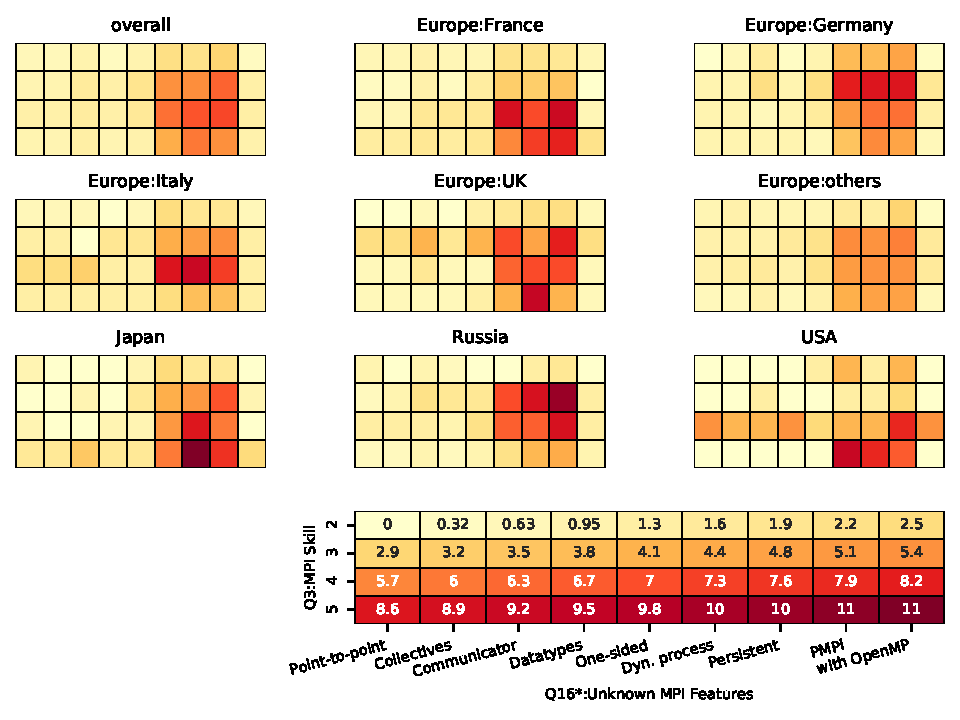
\includegraphics[width=8.0cm]{Figs/Q3-Q16.pdf}
    \caption{Q3-Q16: MPI Skill {\it(single)} and Unknown MPI Features {\it(multiple)}}
    \label{fig:skill-and-aspects}
  \end{center}
\end{figure}

A similar situation can be seen in the cross-tab analysis between Q6 and Q16
(Fig.~\ref{fig:experience-and-aspects}). It would be natural to expect that the
longer the MPI experience, the more familiar the participant should be with
different MPI features and thus less unknown features. However, some
\mcountries\ (France, UK and Japan) show that in some cases there is no
relationship between these two, and that a longer experience could evolve around
the same, limited set of MPI features being used.  This may also indicate that
experienced MPI users may not easily catch up the newly introduced MPI features.

\begin{figure}[tb]
  \begin{center}
    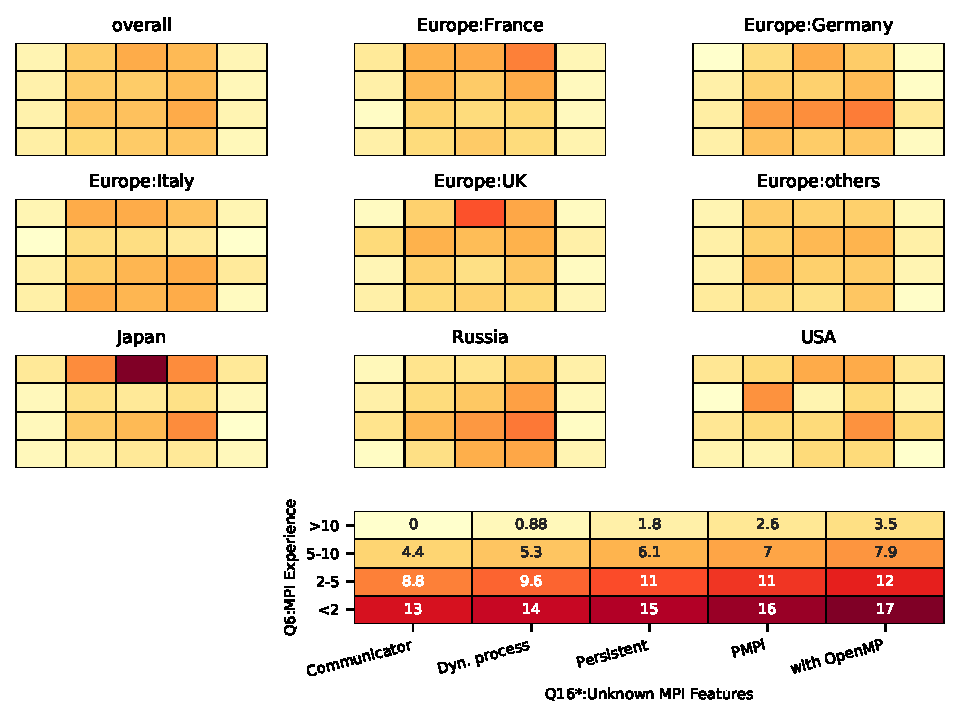
\includegraphics[width=8.0cm]{Figs/Q6-Q16.pdf}
    \caption{Q6-Q16: MPI Experience {\it(single)} and Unknown MPI Features {\it(multiple)}}
    \label{fig:experience-and-aspects}
  \end{center}
\end{figure}

This may indicate that the MPI standard is complex, and its understanding by the
general developer population remains limited. Even the most basic send/receive
functions, although their API looking simple and natural, require deep knowledge
such as possibility of deadlock, timing of buffer access, blocking/non-blocking,
and so on.

Fig.~\ref{fig:useless-features} represent the answers regarding the MPI features
perceived as unnecessary by the participants (Q27: \myquote{What MPI feature(s)
are NOT useful for your application?}). Although most participants believe MPI
has little {\it unnecessary features}, a fair amount of participants seem
convinced that the dynamic process features are not useful. There is certainly a
correlation between this and the fact that dynamic process feature is not being
used by the most participants (Q17, Fig.~\ref{fig:using-mpi-aspects}). It should
be noted that this tendency is also reported in \cite{10.1145/3295500.3356176}.

\begin{figure}[tb]
  \begin{center}
    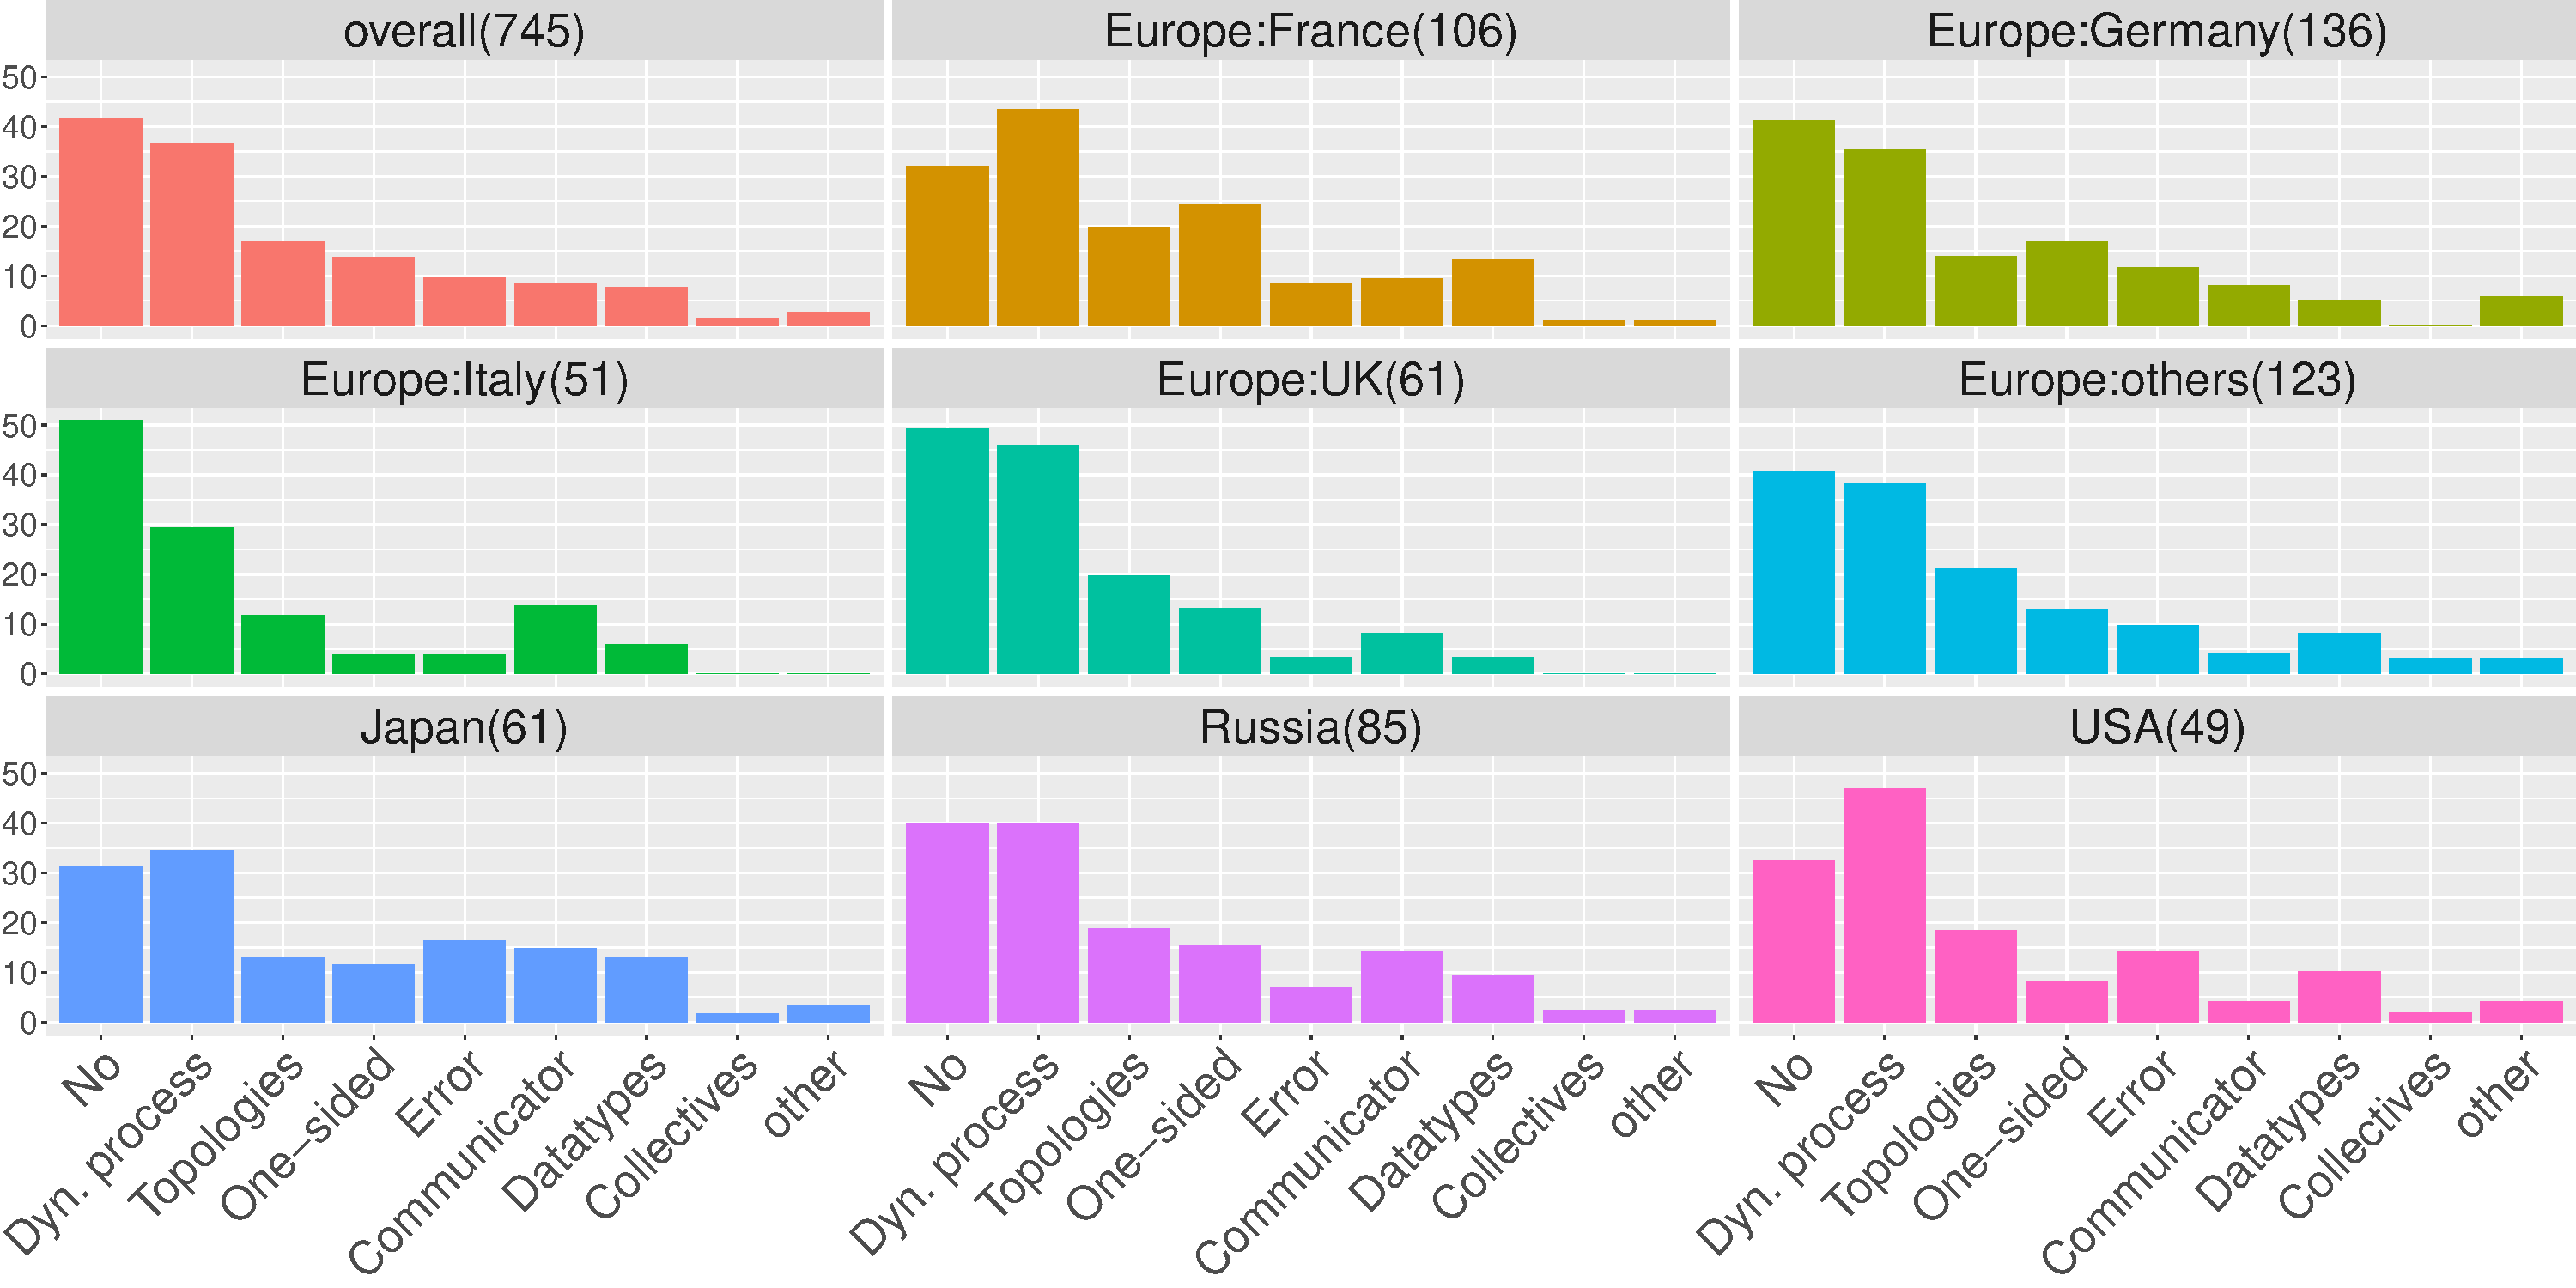
\includegraphics[width=8.0cm]{R-scripts/Q27.pdf}
    \vspace{-2mm}
    \caption{Q27: Useless Features {\it(multiple)}}
    \label{fig:useless-features}
  \end{center}
\end{figure}

The dynamic process feature is on the border of process management and
communication, since the process creation itself is obviously out of the scope
of the MPI standard, while the communication between the existing (MPI)
processes and newly create (MPI) processes must be defined in the standard.
Indeed, the implementation of dynamic process creation \revision{spreads}{involves} many parts of a
computing system: MPI library, process manager, job scheduling system and system
operation.
%
But, we also need to look at applications and their demands. Most of the
scientific applications look at the scientific process on a set of fixed
boundaries and condition, and thus required a fixed number of processes in a
completely static world, one that does not grow or shrink. Few applications exit
this mold, and the small number of developers working around these applications
seem to not have been reached by the survey.

% This complexity might make the use of the dynamic process creation hard and
% impractical for MPI users and the un-usefulness of dynamic process may not come
% from the MPI standard.

\subsection{Multi-threading}\label{sec:mutil-threading}

Similar to dynamic processes, the outcome of the question related to threading
support in MPI has widely divergent answers between the two surveys.
% The difference between our survey and the ECP survey can also be found on
% the question asking multi-threading support.
Fig.~\ref{fig:multi-thread-reg} shows the result of our survey and
Fig.~\ref{fig:multi-thread} shows the difference with the ECP survey. Note that
our question is multiple-choice and the ECP question is single-choice. In both
surveys, the percentage of using {\tt MULTIPLE} is the highest among the valid
choices, but the percentage of the choice \revision{\myquote{I don't know}}{\myquote{No idea}} remains the
largest. This may sound contradictory because the ECP participants would be more
experienced MPI users.

\begin{figure}[tb]
  \begin{center}
    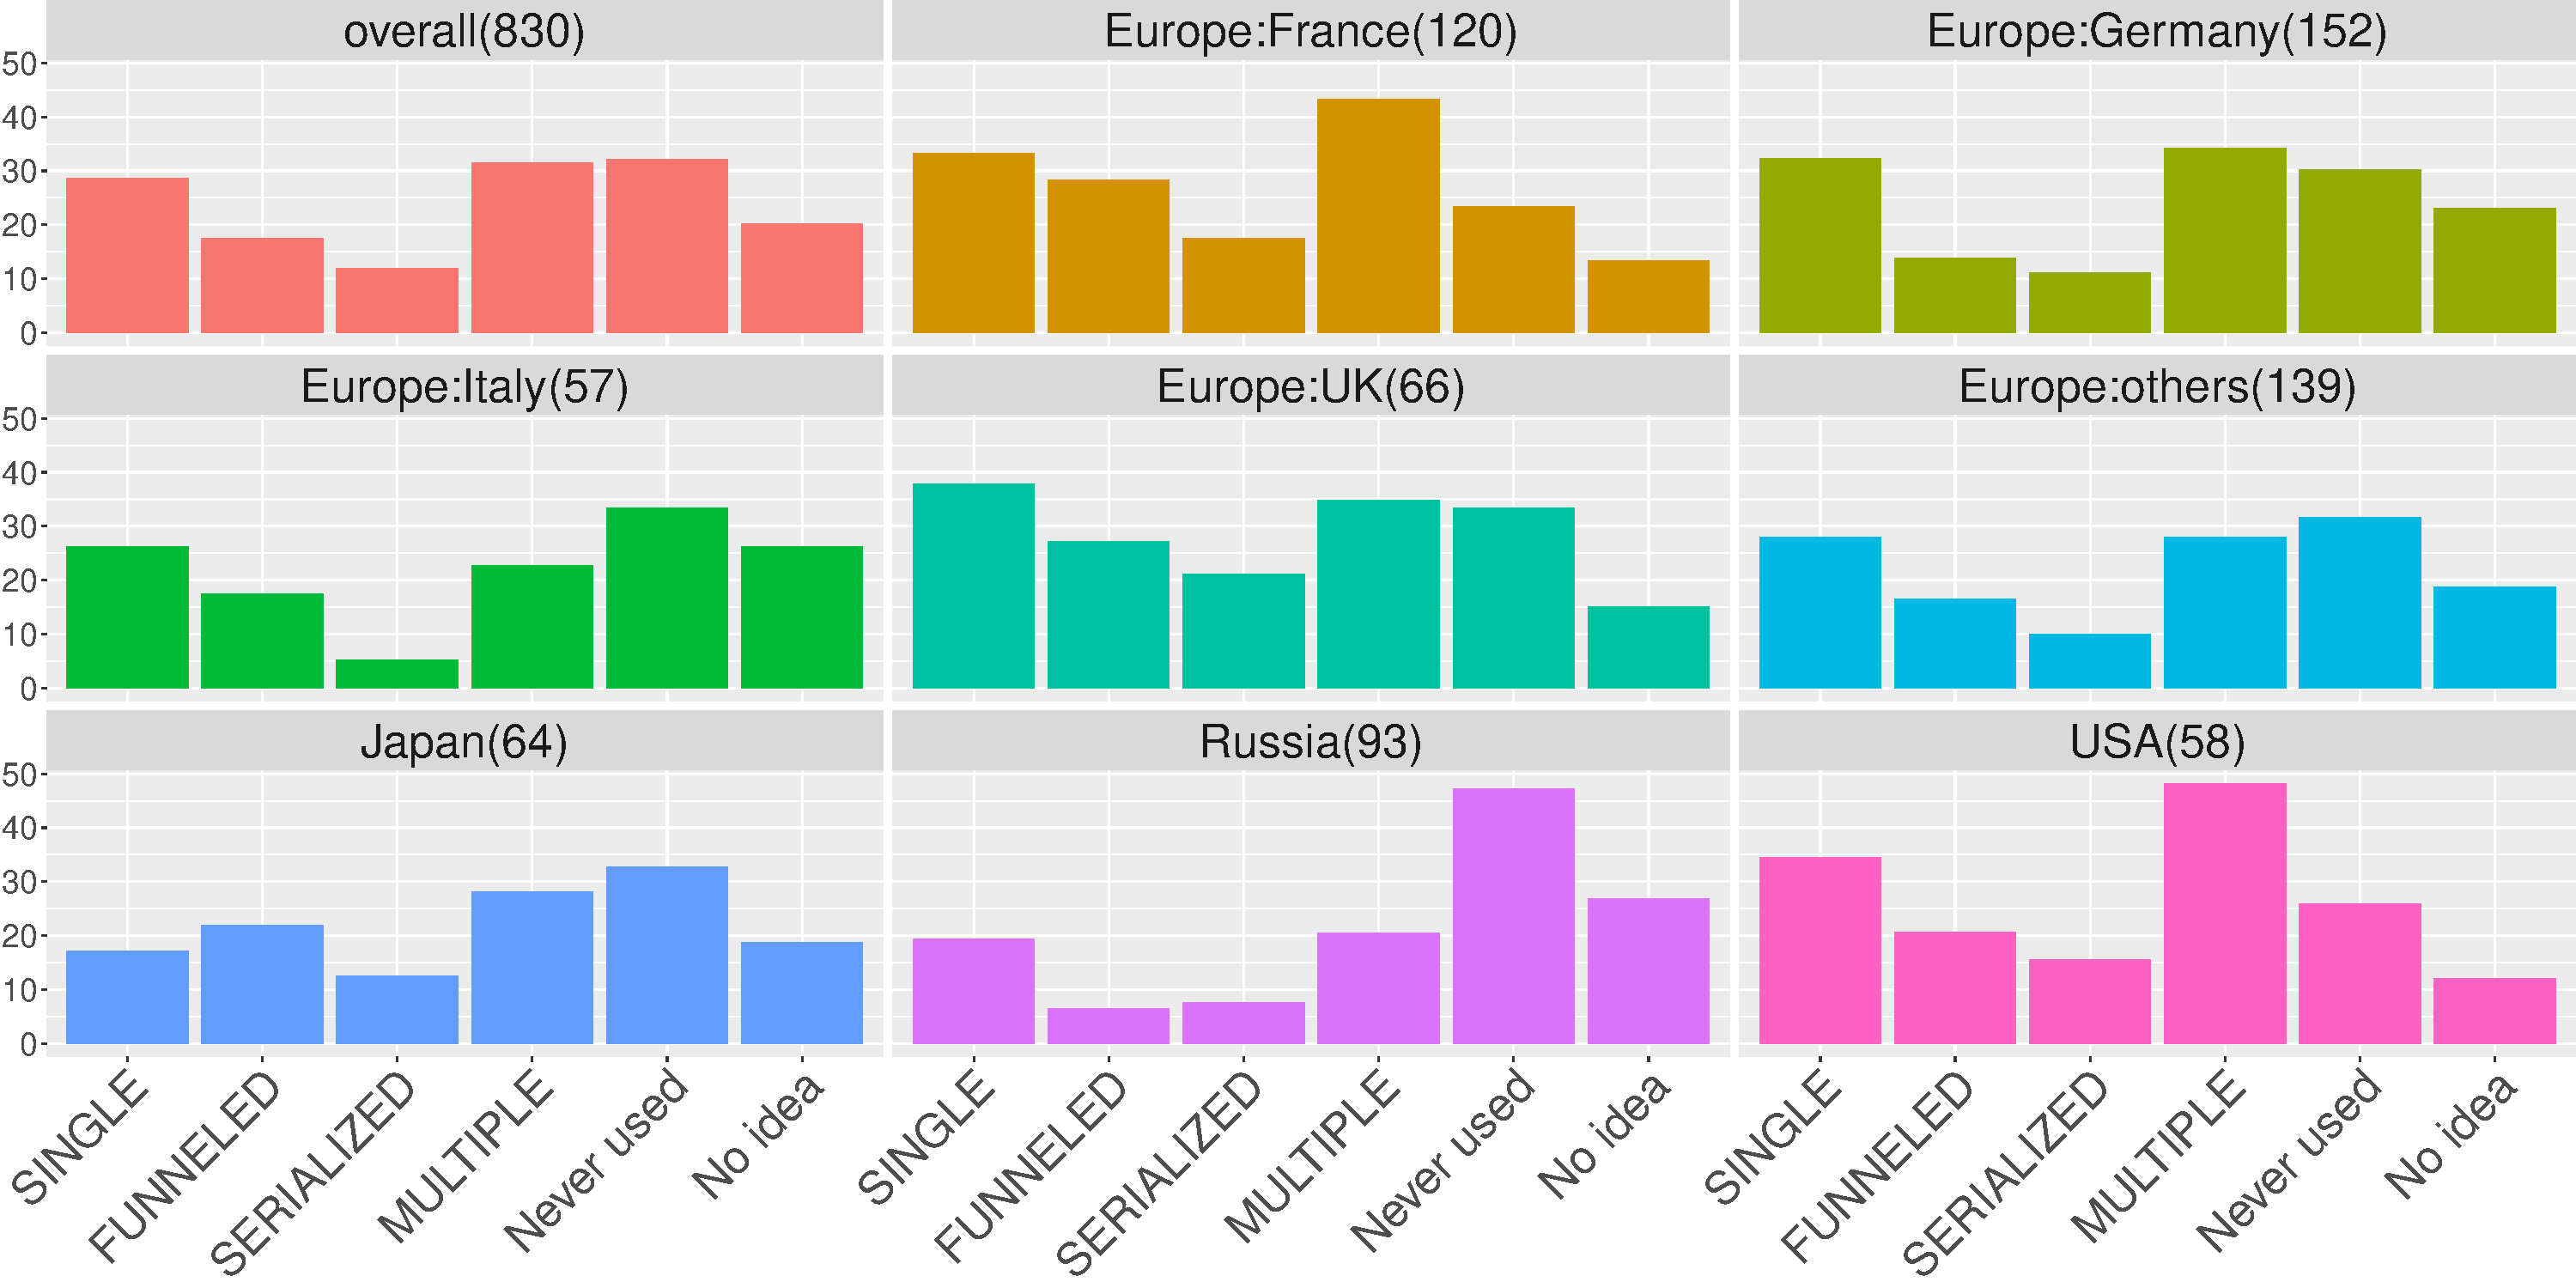
\includegraphics[width=8.0cm]{R-scripts/Q18.pdf}
    \vspace{-2mm}
    \caption{Q18: Multi-threading {\it(multiple)}}
    \label{fig:multi-thread-reg}
  \end{center}
\end{figure}

\revision{
\begin{table}[tb]%
  \small%
  \begin{center}%
    \caption{Multi-threading}\label{tab:multi-thread}%
    \begin{tabular}{c||c|c||c|c|c}%
      \hline%
      Choice & \multicolumn{2}{c||}{Our Survey [\%]} &
      \multicolumn{3}{c}{ECP {\it(single)} [\%]} \\
      \cline{2-6}%
      & overall & USA & AD & ST & AD+ST \\
      \hline%
      SINGLE & 29 & 22 & \multicolumn{3}{c}{\scriptsize (no corresponding choice)} \\
      FUNNELED & 18 & 13 & 18 & 18 & 18 \\
      SERIALIZED & 12 & 10 & 18 & 18 & 18 \\
      MULTIPLE & 22 & 31 & 18 & 32 & 25 \\
      never used & 23 & 16 & \multicolumn{3}{c}{\scriptsize (no corresponding choice)} \\
      not know & 14 & 8 & 25 & 25 & 25\\
      \hline%
    \end{tabular}%
  \end{center}%
\end{table}%
}
{
\begin{figure}[tb]
  \begin{center}
    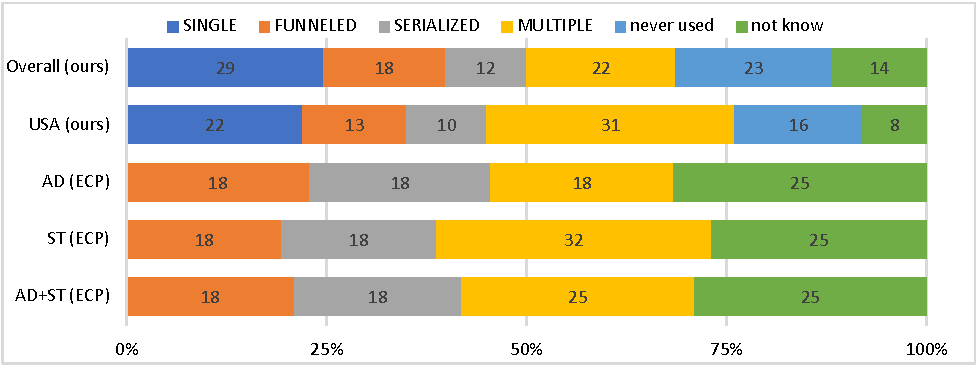
\includegraphics[width=8.5cm]{Figs/MultiThreading-ours-ECP.pdf}\\%
    {\scriptsize ECP does not have the choices \myquote{SINGLE} and
      \myquote{never used}}
    \caption{Multi-threading comparison
      (ECP does not have the choices \myquote{SINGLE} and
      \myquote{never used})}
    \label{fig:multi-thread}%
  \end{center}
\end{figure}
}           

The usage of {\tt MULTIPLE} in US is also the highest among the
\mcountries\ (Fig.~\ref{fig:multi-thread-reg}). France and Germany have
the same trend. In Italy, Japan, Russia and the
other European countries, the percentages of \revision{\myquote{I don't know}}{\myquote{No idea}}
are the highest. In UK, the percentage of using {\tt SINGLE} is the
highest.

Keeping in mind this question was a
\revision{multiple-choice}{multiple-answer} question 
\revision{Table~\ref{tab:multi-thread-raw}}{Fig.~\ref{fig:multi-thread-raw}} shows the top \revision{7}{seven} aw answers
(combined answers \revision{}{, excluding \myquote{never user} and
  \myquote{no idea}}),
with a coverage of about 85\% of the total answers.
% These top 7 percentages occupy about 85\% in total.
As nearly half participants answered \myquote{never used} or \myquote{no idea},
we will ignore these two choices in the remaining of this analysis. This is
reflected in the numbers in parenthesis in this table which are the percentage
of participants excluding those who answered \myquote{never used} or \myquote{no
idea}. Half of threading-aware participants are using {\tt SINGLE} and/or {\tt
MULTIPLE}. Although many participants ignore the thread mode, some participants
use a particular thread support ({\tt SINGLE} or {\tt MULTIPLE}) and some other
participants select one of supported thread capabilities willingly, which might
indicate a well established knowledge of the MPI features.

\revision{
\begin{table}[tb]%
  \begin{center}%
    \caption{Multi-threading - Raw Answers}\label{tab:multi-thread-raw}%
    \begin{tabular}{c|c}%
      \hline%
      Threading Support & Overall \\
      & Percentage \\
      \hline%
      \myquote{never used} + \myquote{no idea} & 48 \\
              {\tt MULTIPLE} & 12 (23) \\
              {\tt SINGLE, MULTIPLE} & 8 (16) \\
              {\tt SINGLE} & 7 (14) \\
              {\small\tt SINGLE, FUNNELED, SERIALIZED, MULTIPLE} & 4 (8) \\
              {\tt SINGLE, FUNNELED} & 3 (7) \\
              {\tt SERIALIZED} & 3 (5) \\
              \hline%
              \multicolumn{2}{c}{\footnotesize Numbers in parenthesis are
                percentages excluding \myquote{never used} and \myquote{no
                  idea}}
    \end{tabular}%
  \end{center}%
\end{table}%
}
{
\begin{figure}[tb]
  \begin{center}
    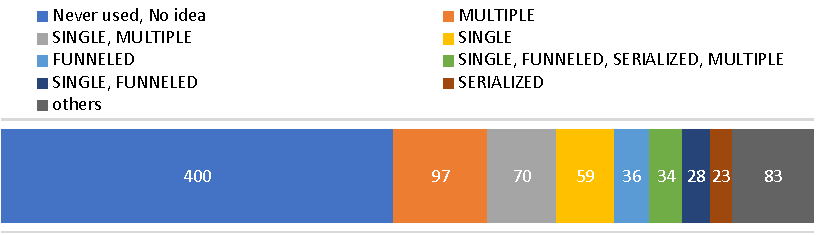
\includegraphics[width=8.0cm]{Figs/MultiThreading-raw.pdf}
    \vspace{-2mm}
    \caption{Multi-threading - Raw Answers}\label{tab:multi-thread-raw}%
    \label{fig:multi-thread-raw}%
  \end{center}
\end{figure}
}

A similarly scattered trend has also been confirmed by other studies. Indeed,
\cite{8665758} indicates approximately 75\% of their target executables (not
number of jobs) on Mira (total of 68) are using {\tt SINGLE}, 15\% use {\tt
FUNNELED} and 4\% use {\tt MULTIPLE}. Similarly, \cite{10.1145/3295500.3356176}
indicate that approximately 60\% of their target programs use {\tt FUNNELED},
30\% use {\tt MULTIPLE}, 20\% use {\tt SINGLE} and only few percent use {\tt
SERIALIZED}. Thus, the thread support usage varies on each survey and further
investigation is needed to state a result.

\section{Other Findings}

\subsection{MPI Implementations}

 Fig.~\ref{fig:using-implementations} shows the usage of the different MPI
 implementations, (Q12 asking specifically which MPI implementation(s) the
 participants are using regularly). This result presents a coherent picture
 across the board, as Open~MPI, Intel MPI and MPICH, dominates \revision{in}{for} all
 \mcountries\ followed by MVAPICH. Outside these top contenders, a large
 disparity can be seen on the other implementations. Taking a look at the
 \myquote{other} choice, there are four (4) answers naming the \myquote{bullx
 MPI} and another four (4) using MadMPI~\cite{madmpi} in France, and 10 answers
 raising ParaStation MPI in Germany. The frequency of using Fujitsu MPI,
 ParaStation MPI, bullx MPI and others heavily depend on countries of
 participants and the countries where the MPI was developed.

  \begin{figure}[tb]
    \begin{center}
      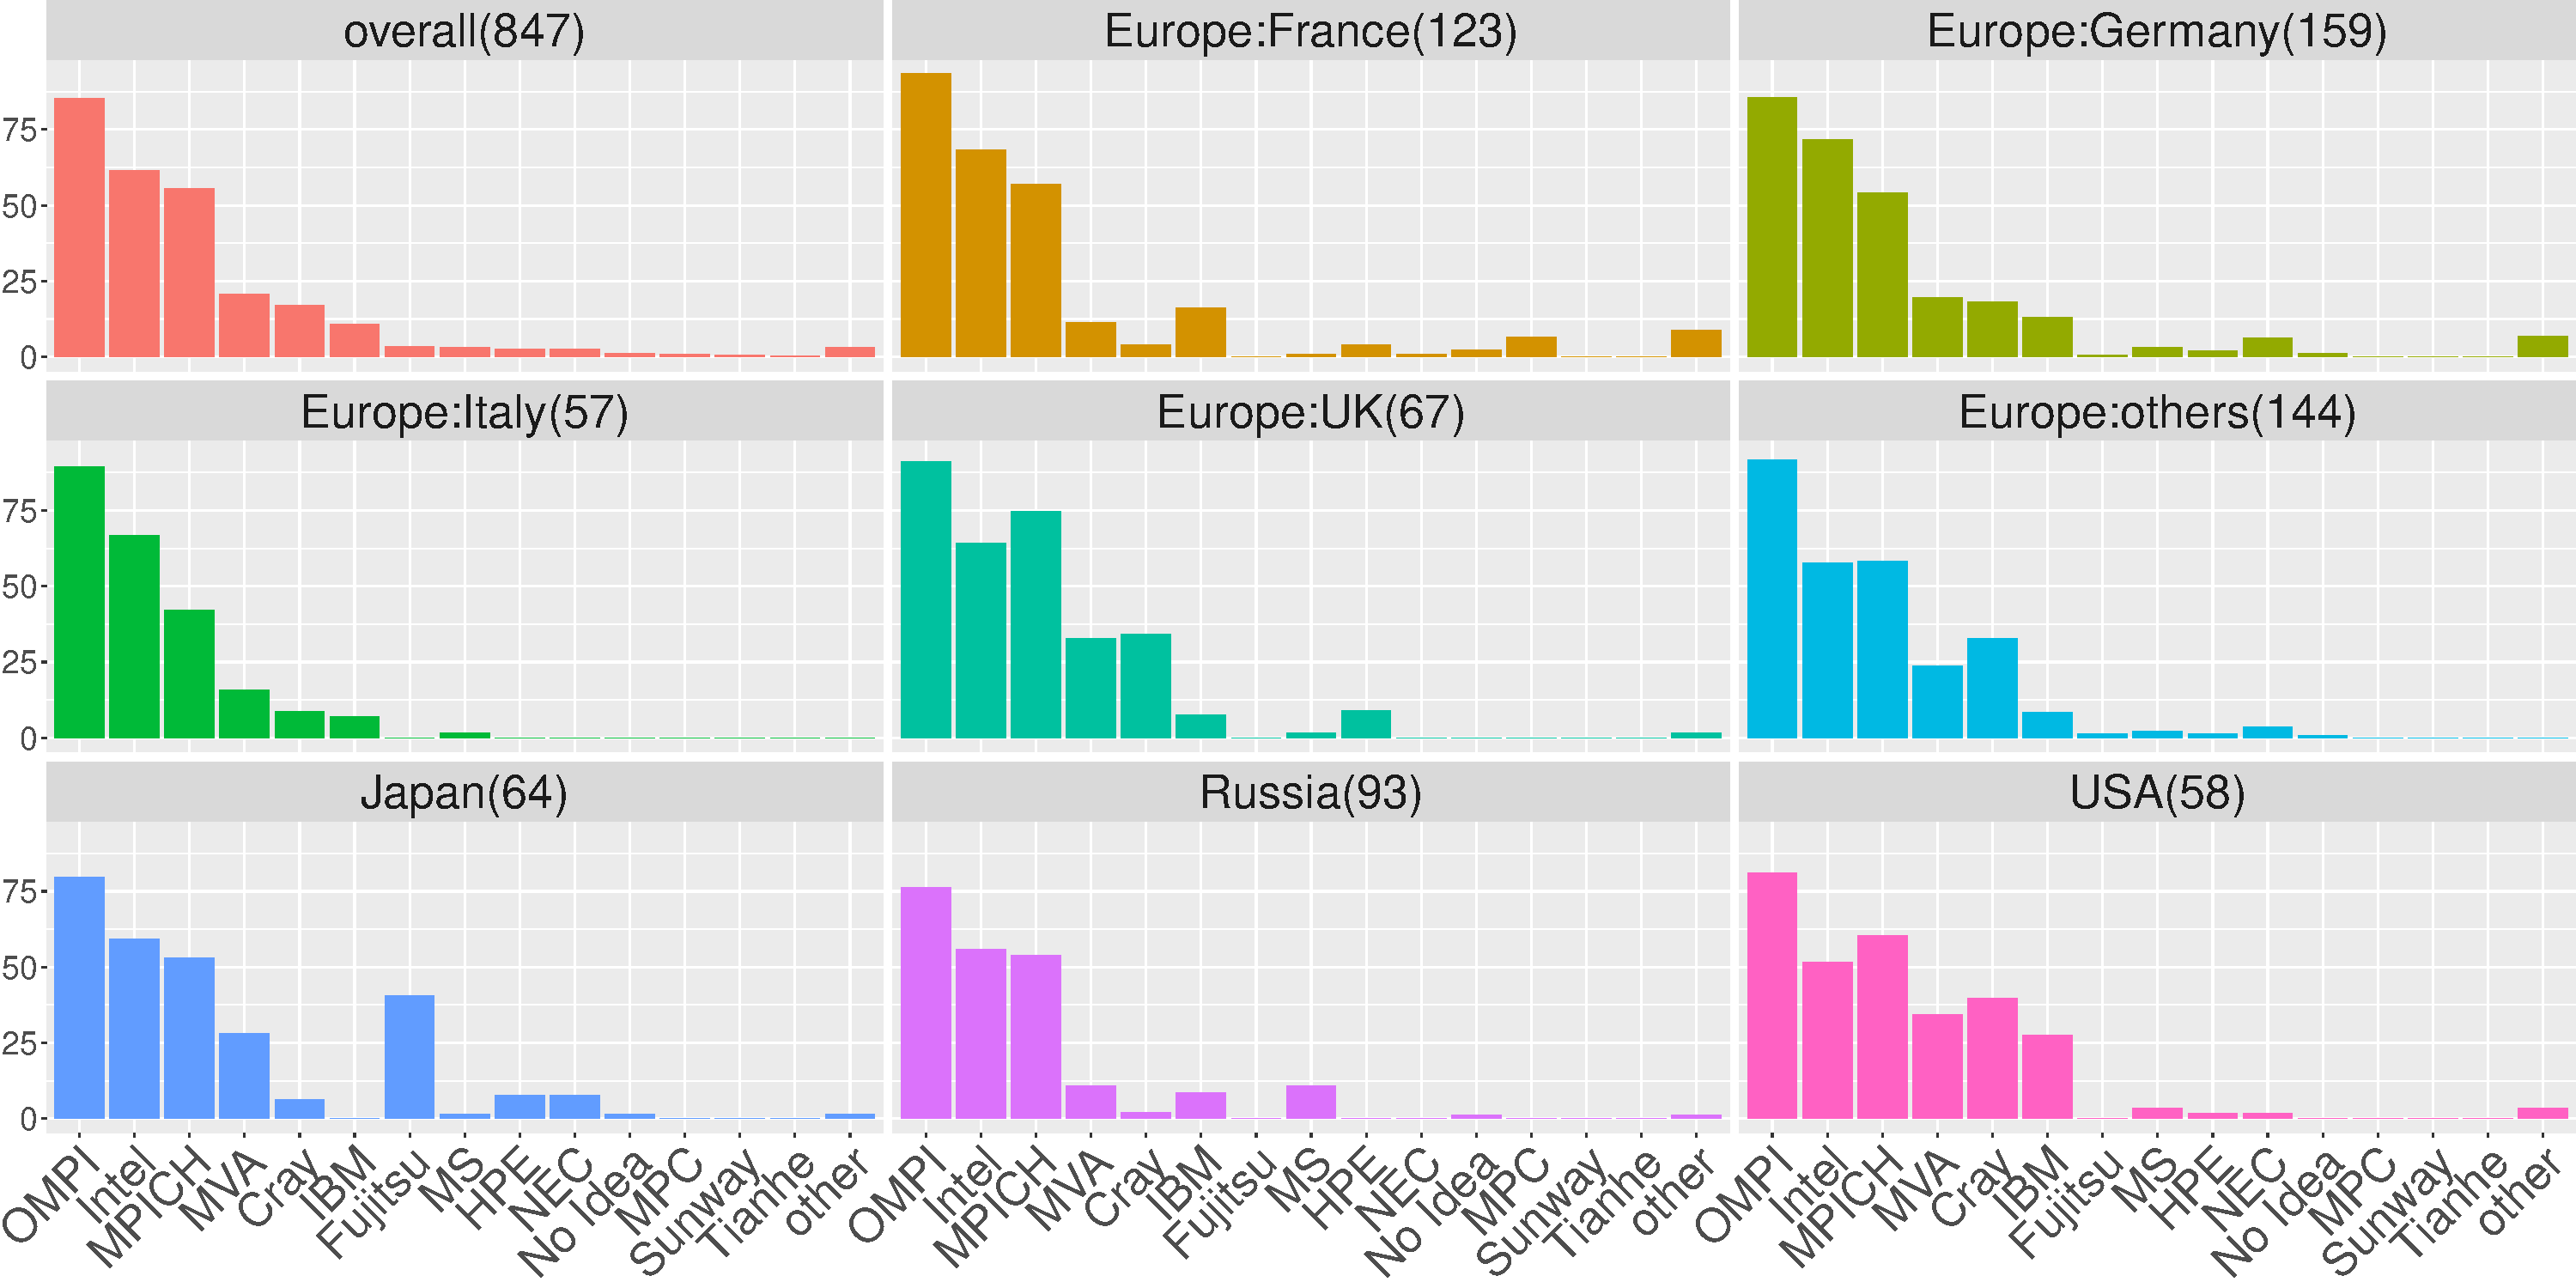
\includegraphics[width=8.0cm]{R-scripts/Q12.pdf}
    \vspace{-2mm}
      \caption{Q12: Using MPI Implementations {\it(multiple)}}
      \label{fig:using-implementations}
    \end{center}
  \end{figure}

In order to understand how the usage of a particular MPI implementation came to
happen, we specifically asked the participants in Q13 \myquote{why did you
choose the MPI implementation(s)} and the answers are shown in
Fig.~\ref{fig:choosing-implementation}.
%
One of the interesting outcomes from this question is the fact that more than
half of the participants outside US have little to no choice in the selection of
the MPI implementation, they have to use what is made available to them with the
platform. For the rest of participants their choice seem to favor their
familiarity with a particular implementation or past experiences with the
community supporting their choice MPI implementation.
%
This clearly suggest that MPI implementors must carefully build and support
their \revision{users}{user} community in order to increase the usage of their particular
implementation.

% The highest percentage of US participants selected \myquote{Familiar}. Many
% Italian participants also selected \myquote{Familiar.} Many Russian
% participants selected \myquote{No reason.} The largest part of UK and Germany
% participants selected \myquote{No choice.} In general, more than half of
% participants excepting US select MPI implementation(s) without any reason nor
% freedom of choice.

  \begin{figure}[tb]
    \begin{center}
      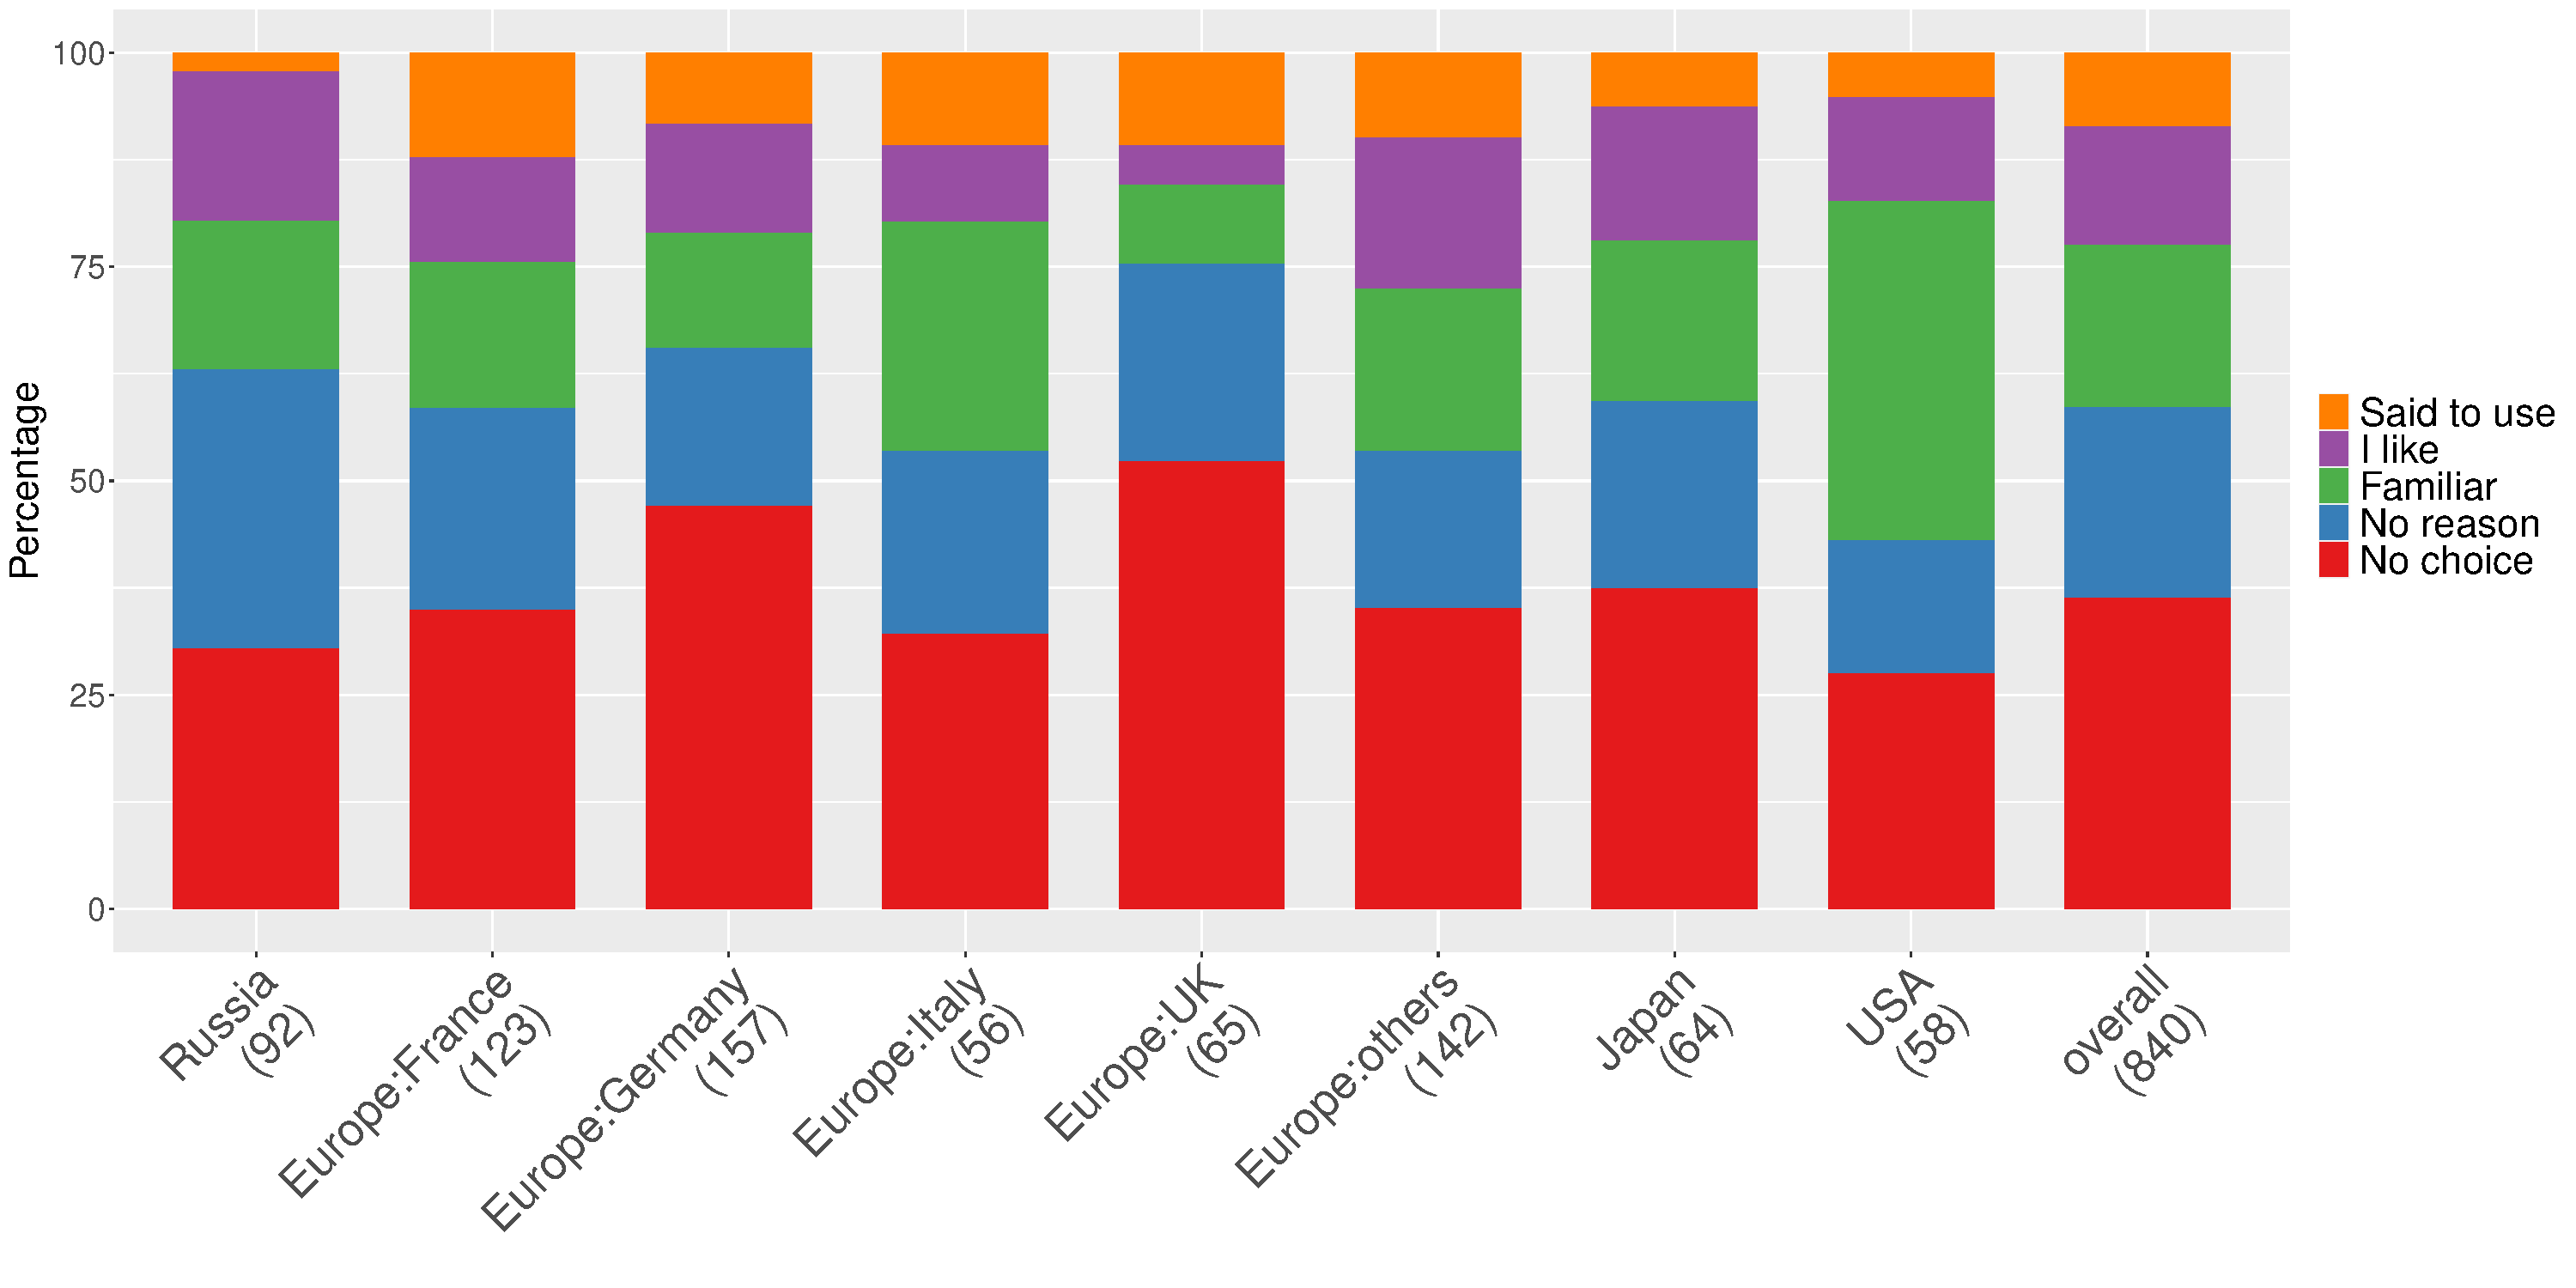
\includegraphics[width=8.0cm]{R-scripts/Q13.pdf}
      \vspace{-2mm}
      \caption{Q13: Choosing MPI Implementations {\it(single)}}
      \label{fig:choosing-implementation}
    \end{center}
  \end{figure}

\subsection{MPI+X and Alternatives}

Fig.~\ref{fig:mpi-x} shows the result of Q22 asking \myquote{Have you ever
written MPI+''X'' programs?}. As a constant across the board, most participants
have \revision{experienced}{experience with} writing MPI+OpenMP programs. An interesting highlight, in US
\myquote{CUDA} is the second largest and the percentage pure MPI applications is
the lowest. Considering the low percentage of \myquote{No} in overall (approx.
25\%), 3/4 participants are using MPI in combination with another, node-level or
accelerator-focused, programming paradigm. A similar finding was highlighted
in~\cite{10.1145/3295500.3356176}, where it has been reported that the
approximately 3/4 of the target programs use the hybrid model of MPI+OpenMP.

\begin{figure}[tb]
\begin{center}
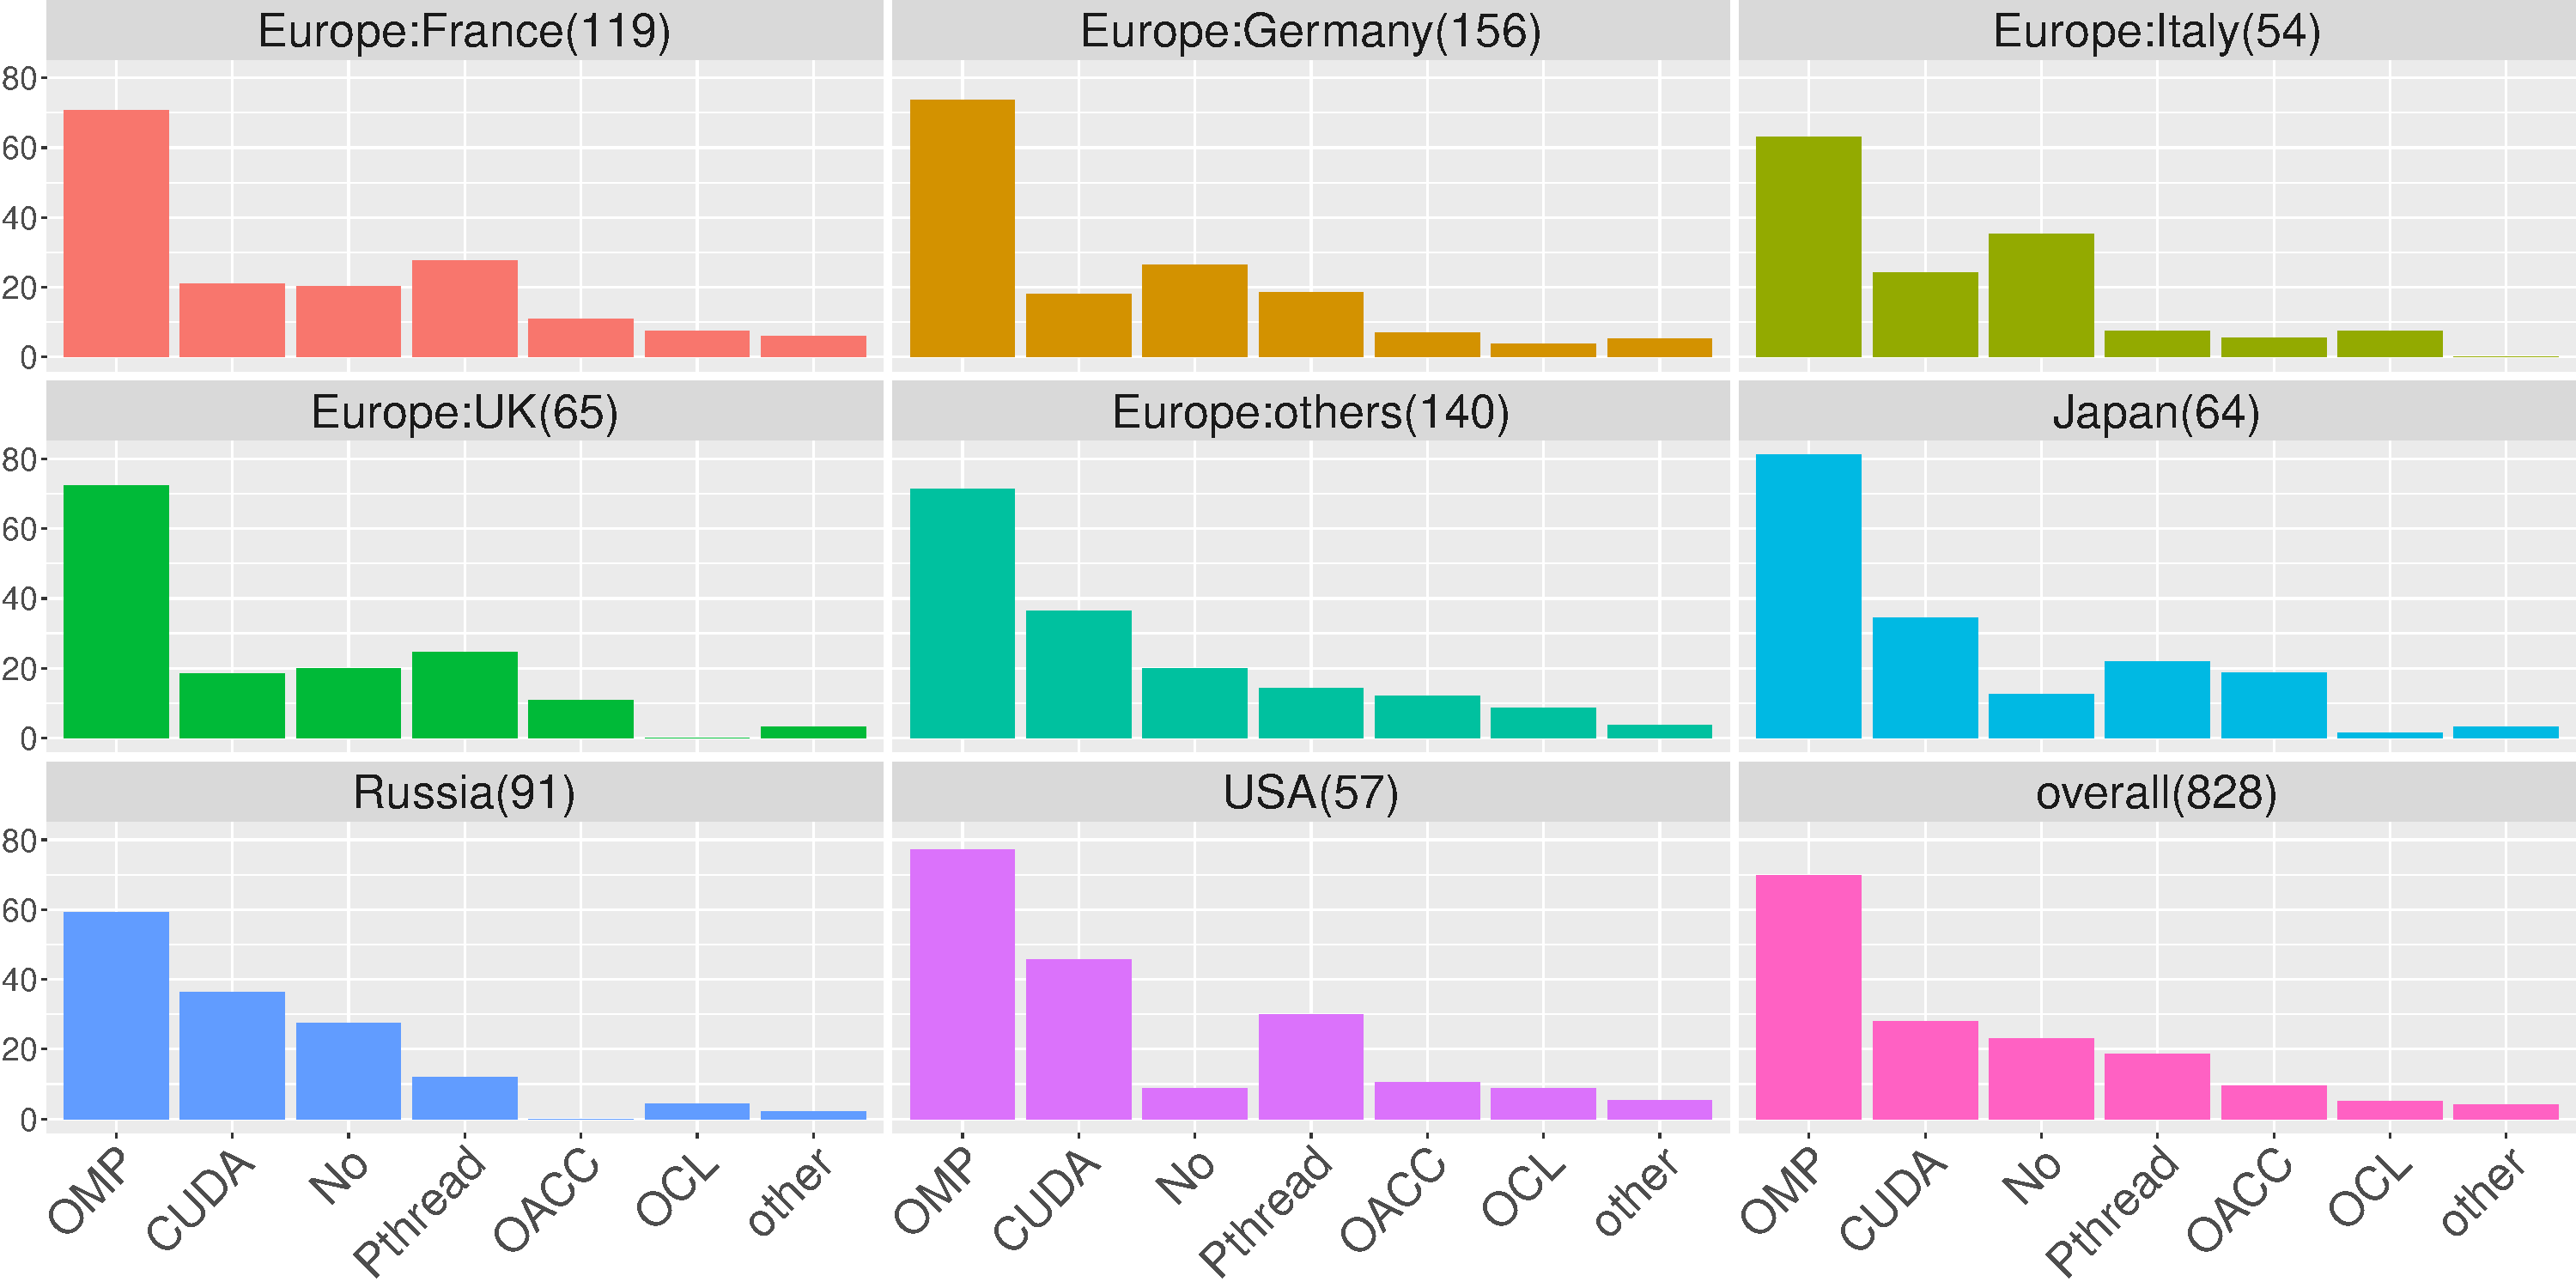
\includegraphics[width=8.0cm]{R-scripts/Q22.pdf}
\vspace{-2mm}
\caption{Q22: MPI+X {\it(multiple)}}
\label{fig:mpi-x}
\end{center}
\end{figure}

\begin{figure}[tb]
\begin{center}
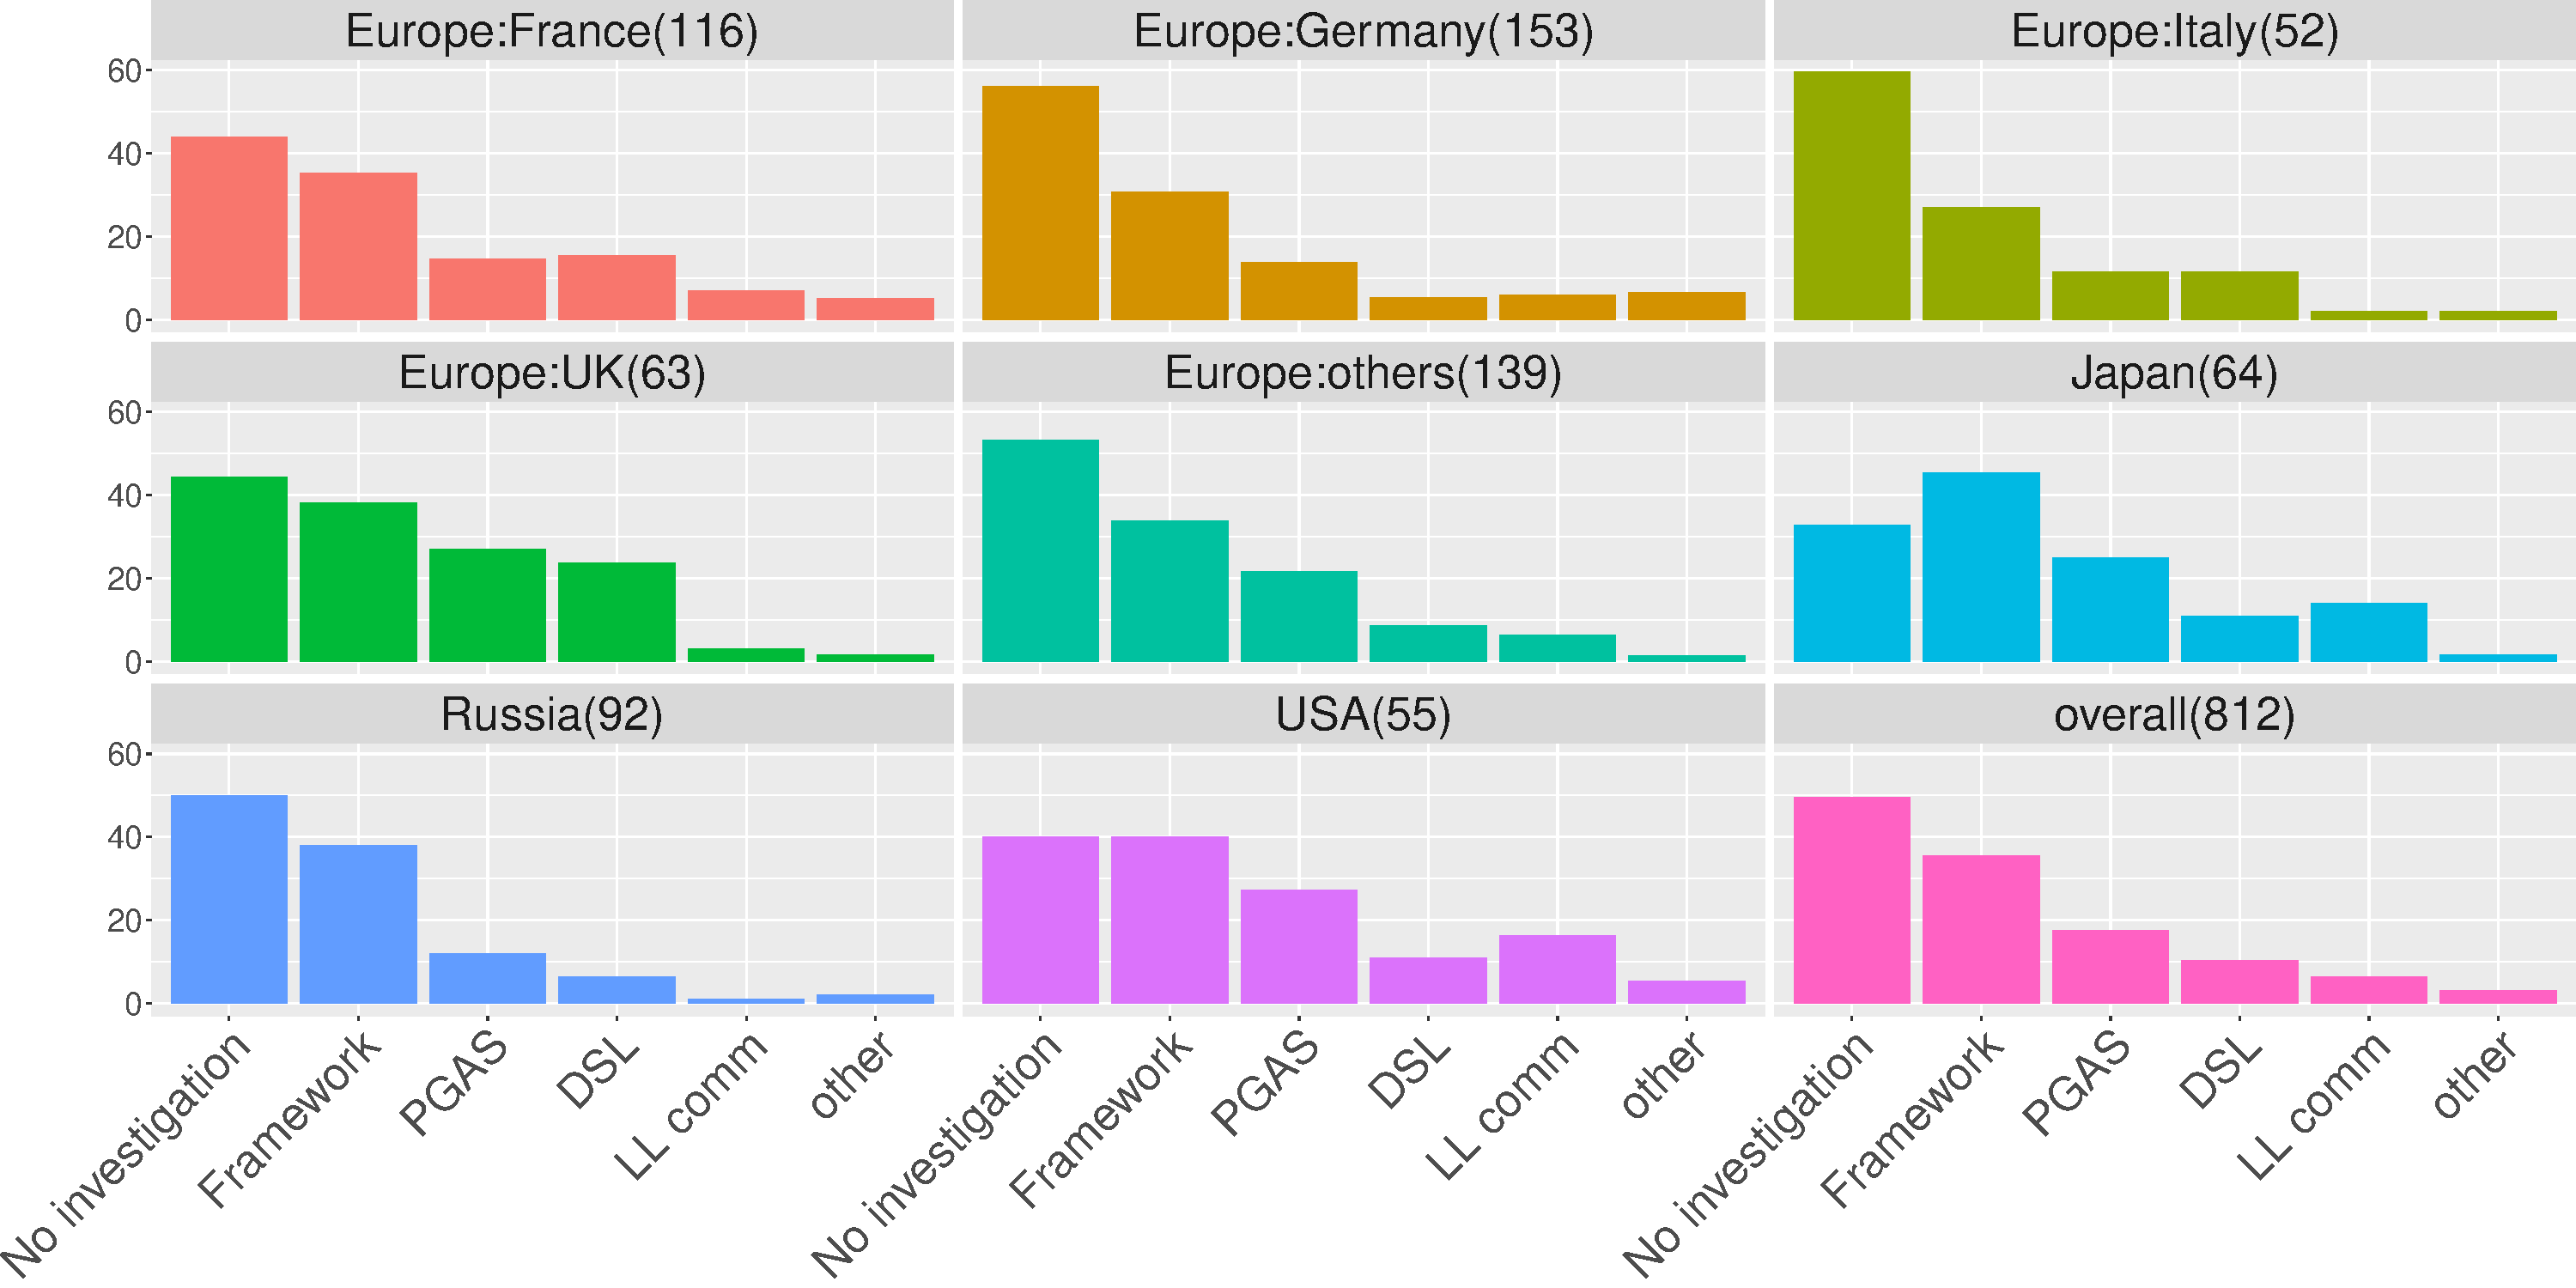
\includegraphics[width=8.0cm]{R-scripts/Q24.pdf}
\vspace{-2mm}
\caption{Q24: MPI Alternatives {\it(multiple)}}
\label{fig:mpi-alternatives}
\end{center}
\end{figure}

Without going in details about the features provided by MPI, it could be natural
to assume that all types of data movements can be provided by other message
passing paradigms. We specifically asked the participants to indicate if they
have investigated any of these alternative message passing libraries (Q24
\myquote{What, if any, alternatives are you investigating to indirectly call MPI
or another communication layer by using another parallel language library?}).
The Fig.~\ref{fig:mpi-alternatives} highlights that almost half of the
participants are totally satisfied with MPI, and have not investigated any
replacement message passing paradigm. Out of the remaining participants,
\myquote{PGAS} seems to be the most used alternative to MPI, a result that is
similar across all \mcountries.

% When the participants were asked the question \myquote{What, if any,
% alternatives are you investigating to indirectly call MPI or another
% communication layer by using another parallel language~/ library?}, they
% exhibited as shown in Fig.~\ref{fig:mpi-alternatives}. In overall,
% almost half participants do not investigate the alternatives. The second
% largest answer was \myquote{Framework} (i.e. a framework or library
% using MPI) followed by \myquote{PGAS}. The
% differences over the \mcountries\  are not so big.

\begin{figure}[tb]
\begin{center}
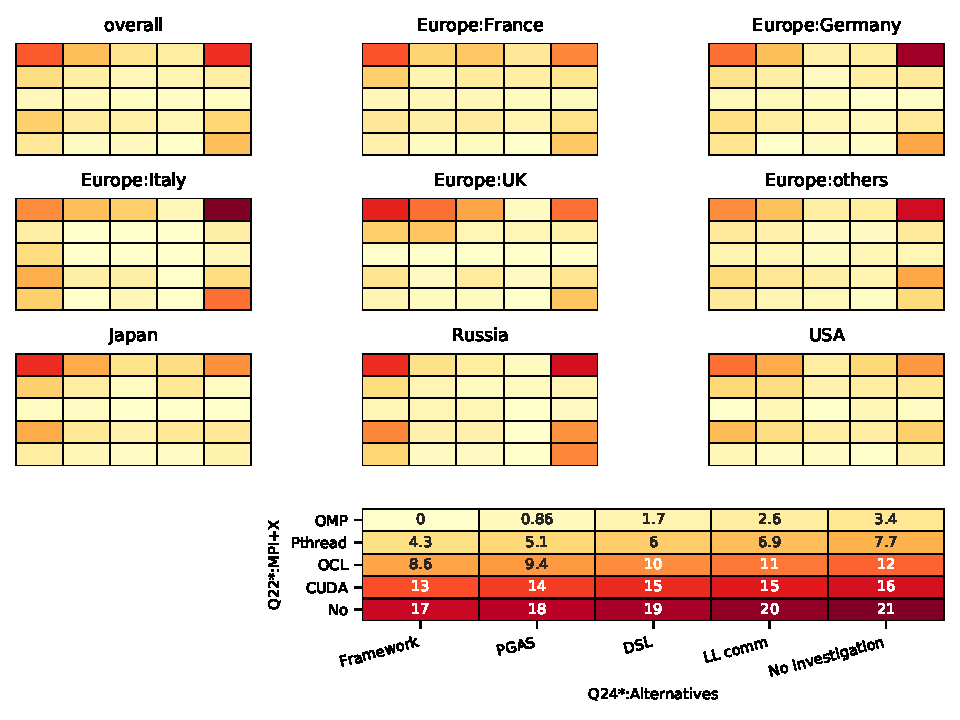
\includegraphics[width=8.0cm]{Figs/Q22-Q24.pdf}
\caption{Q22-Q24: MPI+X {\it(multiple)} and MPI Alternatives {\it(multiple)}}
\label{fig:mpi-x-and-alternatives}
\end{center}
\end{figure}

Fig.~\ref{fig:mpi-x-and-alternatives} shows the cross-tab analysis of Q22 and
Q24. A certain percentage of participants of Germany, Italy, Russia and other
European countries are using hybrid programming (MPI+\ OpenMP) but without
investigating \revision{the}{an} MPI alternative (upper right corners of the heatmaps).

\subsection{Compatibility vs. Performance}

\revision{In the history of MPI, portability, which translates into maintaining backward
compatibility across versions, has been of paramount importance. From the MPI
standard point of view it}{From the MPI
standard point of view, the backward compatibility} can also be an
obstacle to the introduction of new 
features to enhance MPI capabilities, and to the deprecation of features that
proved inconsistent or were replaced by \revision{}{a} better alternative.
Fig.~\ref{fig:performance-vs-compatibility} shows the result of the question
asking which is more important, performance or compatibility on a scale, while
Fig.~\ref{fig:compatibility} shows the expressed need for backward compatibility
(Q28).

\begin{figure}[tb]
\begin{center}
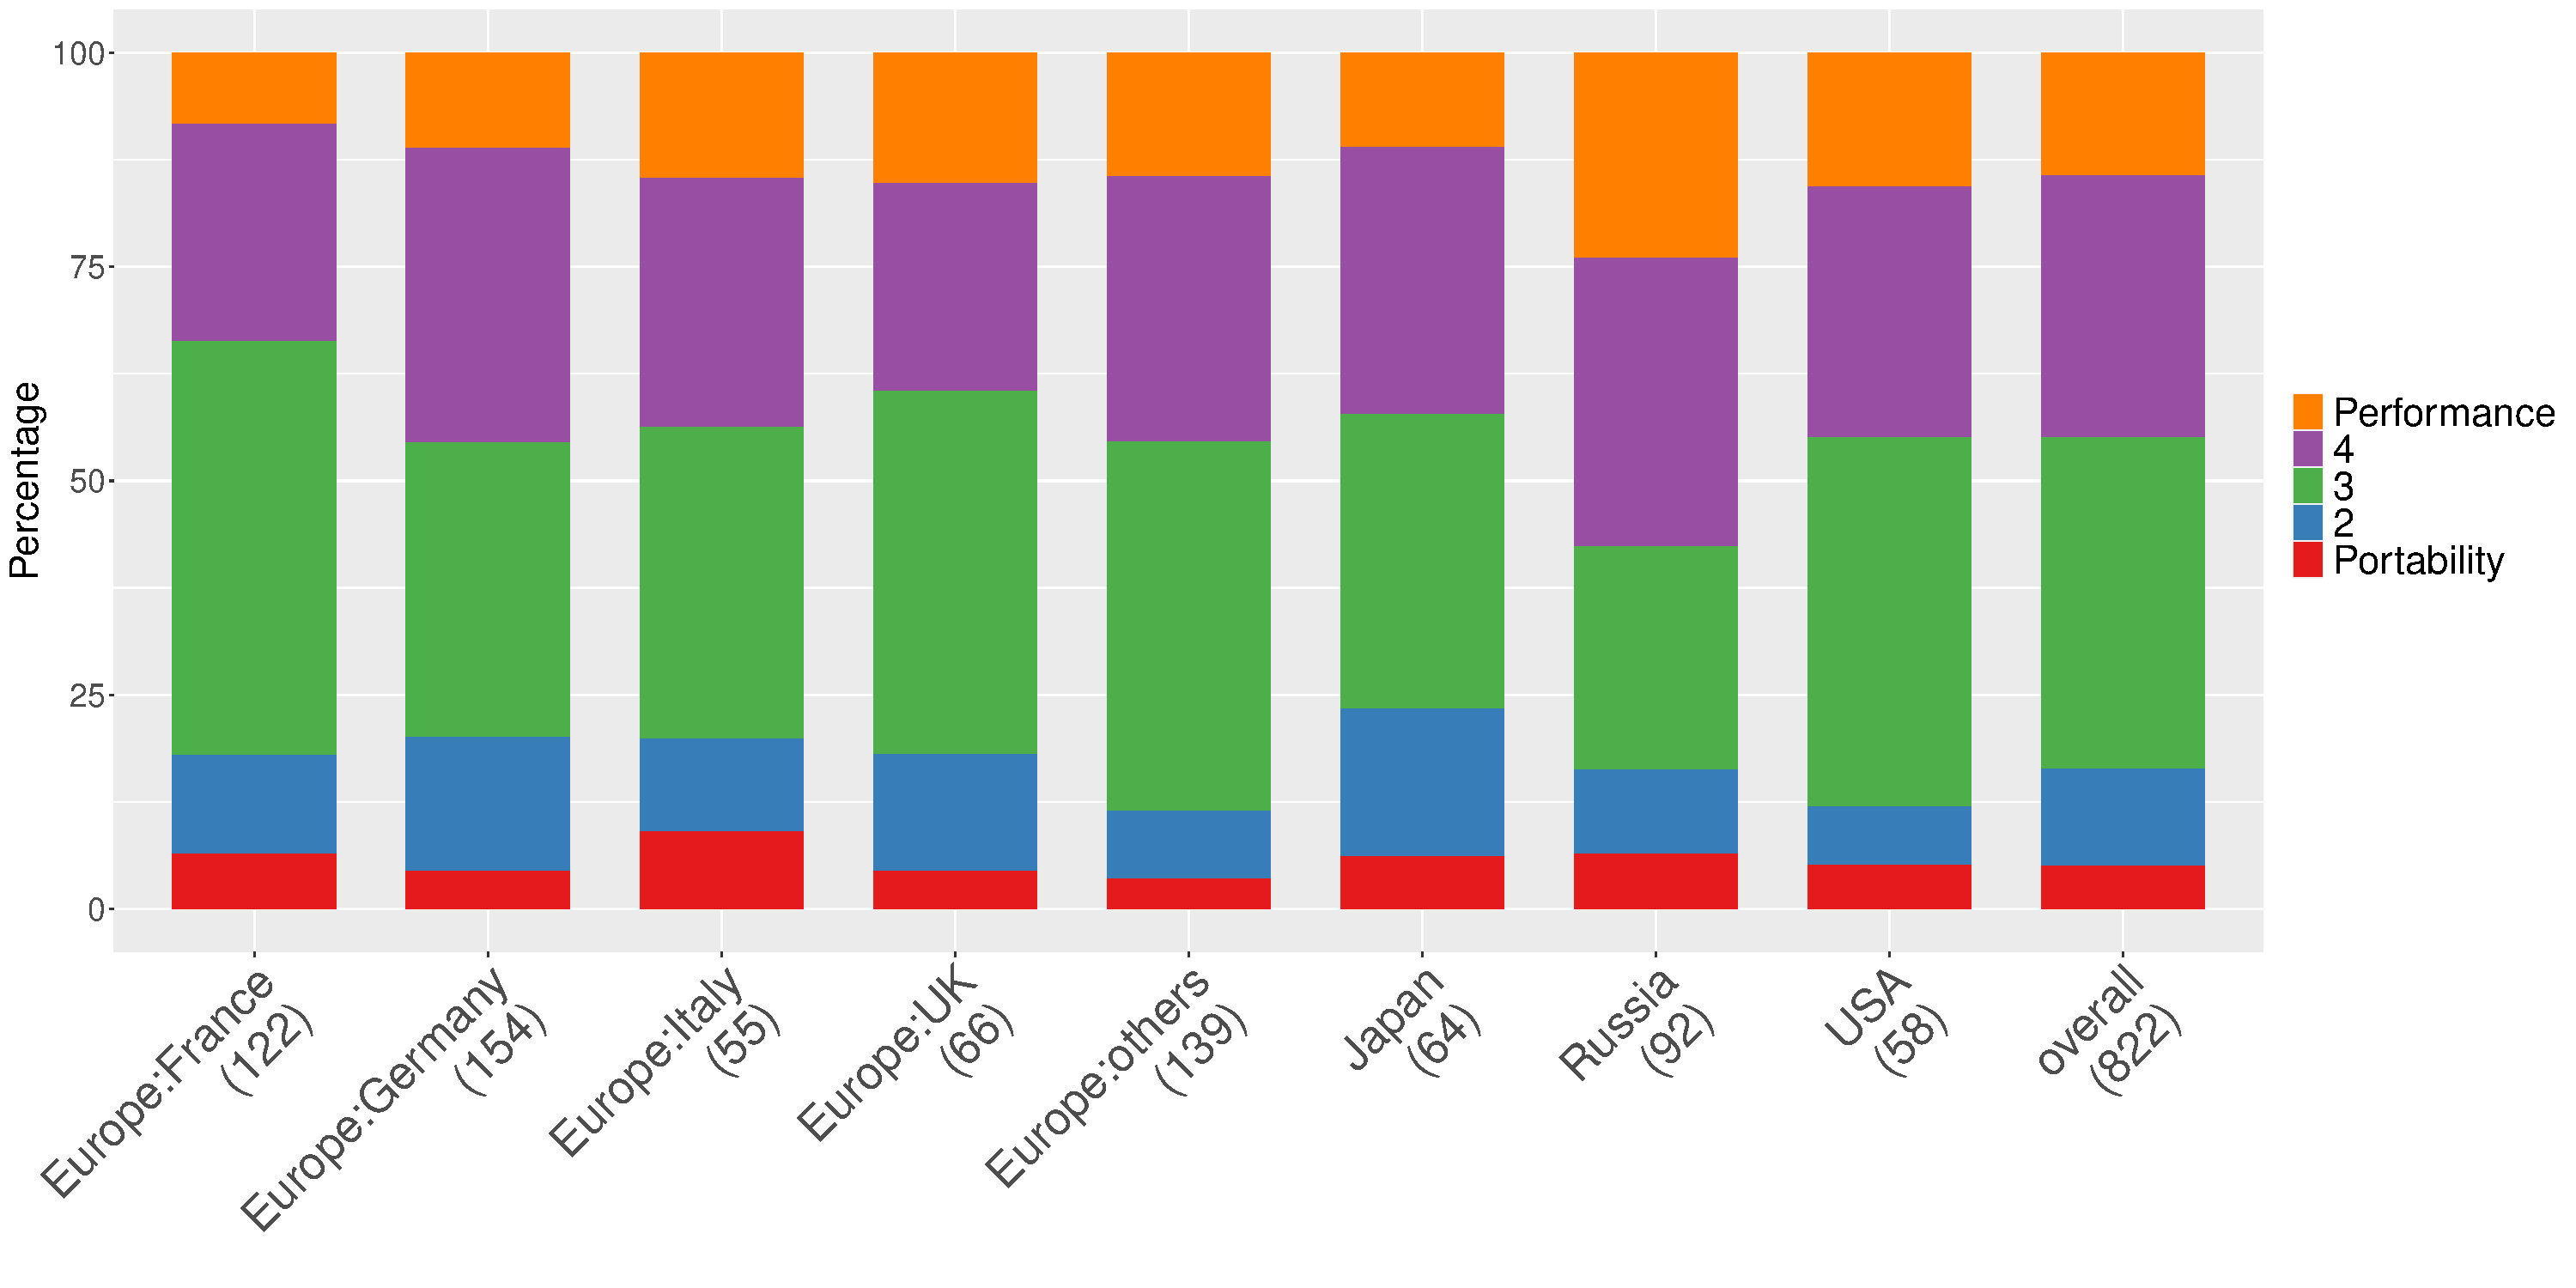
\includegraphics[width=8.0cm]{R-scripts/Q29.pdf}
\vspace{-2mm}
\caption{Q29: Performance vs. Compatibility {\it(single)}}
\label{fig:performance-vs-compatibility}
\end{center}
\end{figure}

In Fig~\ref{fig:performance-vs-compatibility}, let's consider three groups; {\it
performance group} focused on \myquote{Performance} or \myquote{4}, {\it
compatibility group} focused on \myquote{Portability} or \myquote{2}), and {\it
middle group} \revision{who}{that} chose \myquote{3}. While the middle group, striking a balance
between performance and compatibility dominates in most \mcountries\  (\revision{excepting}{except}
Russia), the performance group tend to occupy a larger percentage. Regarding
Russia, a large percentage of Russian participants answered \myquote{my program
is too small} in Q21 (Fig.~\ref{fig:layering-mpi-calls}), in which case the lost
of compatibility does not cause a considerable burden.

\begin{figure}[tb]
\begin{center}
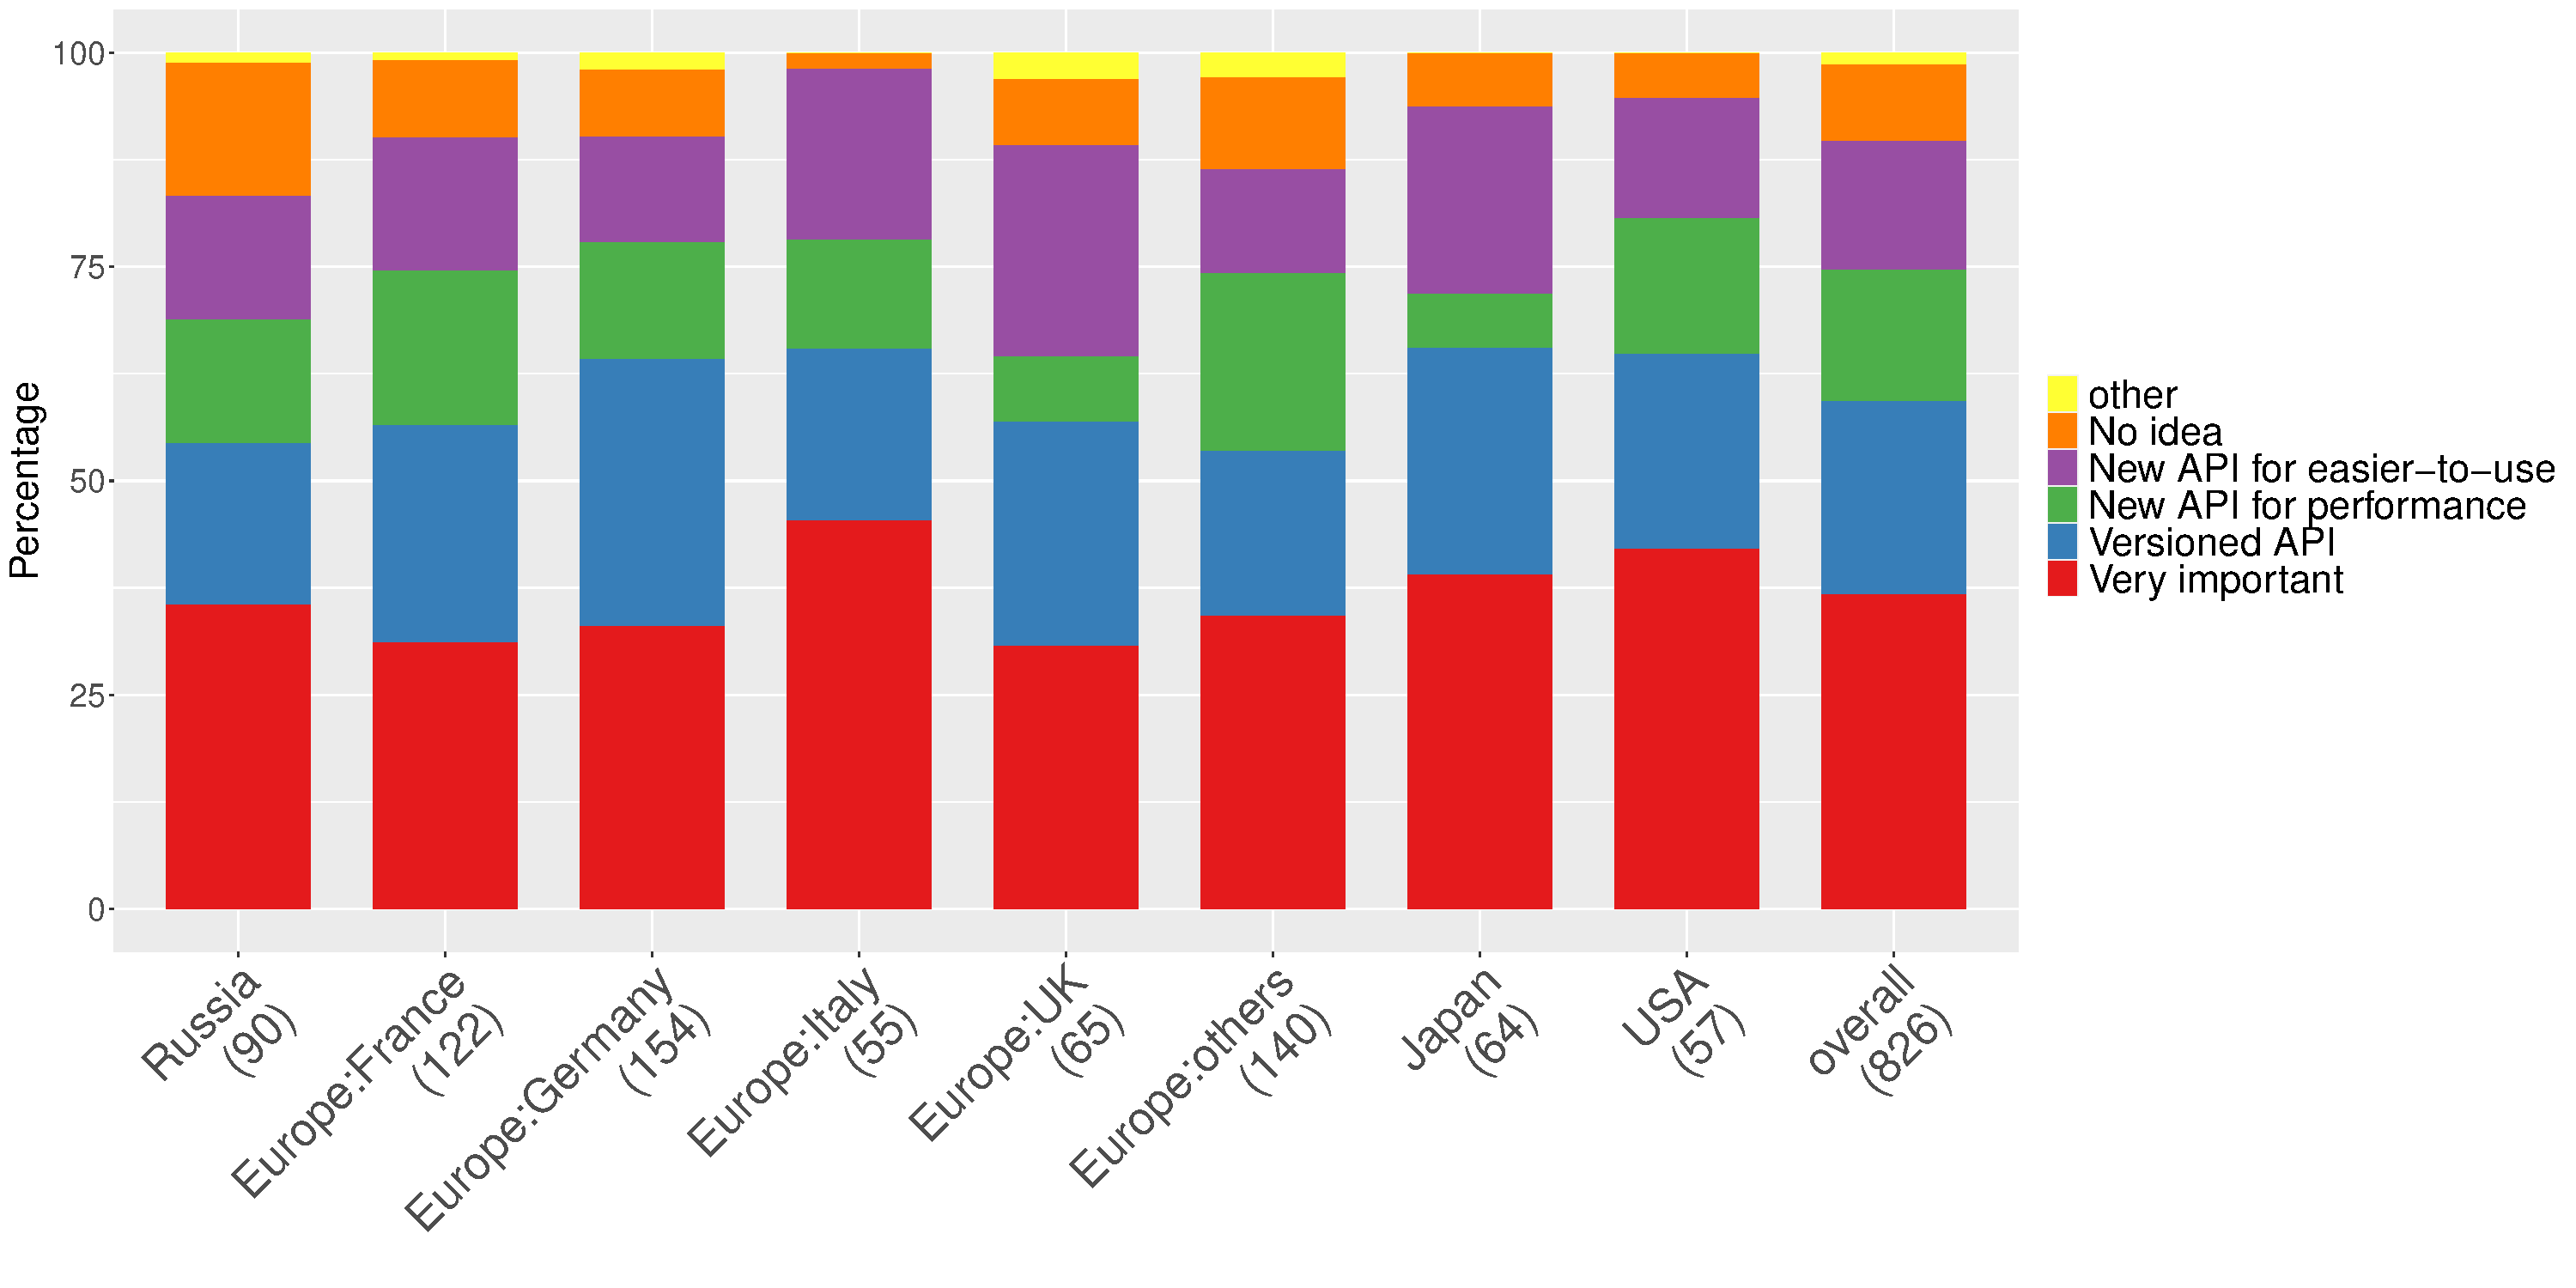
\includegraphics[width=8.0cm]{R-scripts/Q28.pdf}
\vspace{-2mm}
\caption{Q28: Backward Compatibility {\it(single)}}
\label{fig:compatibility}
\end{center}
\end{figure}

As shown in Fig.~\ref{fig:compatibility}, around 40\% of participants answered
that the compatibility is very important, while the rest of participants may
accept the \revision{incompatibility}{incompatibilities} conditionally. The incompatibility forces users to
update their programs. The result of Q28 may \revision{suggests}{suggest} that users would accept
incompatibility in exchange \revision{of}{for} a substantiated benefit, either in terms of
performance or productivity.

\subsection{Learning MPI}\label{sec:learning-mpi}

Fig.~\ref{fig:learning-mpi} shows the percentages of how participants learned
MPI. In this graph, \myquote{Other lec.} indicates the choice \myquote{Other
lectures or tutorials (workplace, conference)}. The UK and Russia participants
preferred to learn from online sources. The participants of Germany and other
European countries preferred to have other form of lectures. The percentage of
reading \myquote{Books} in US is the highest. Taking a look at the other
answers, 18 participants learned by reading existing code and 8 participants
learned by writing MPI applications.

\begin{figure}[tb]
\begin{center}
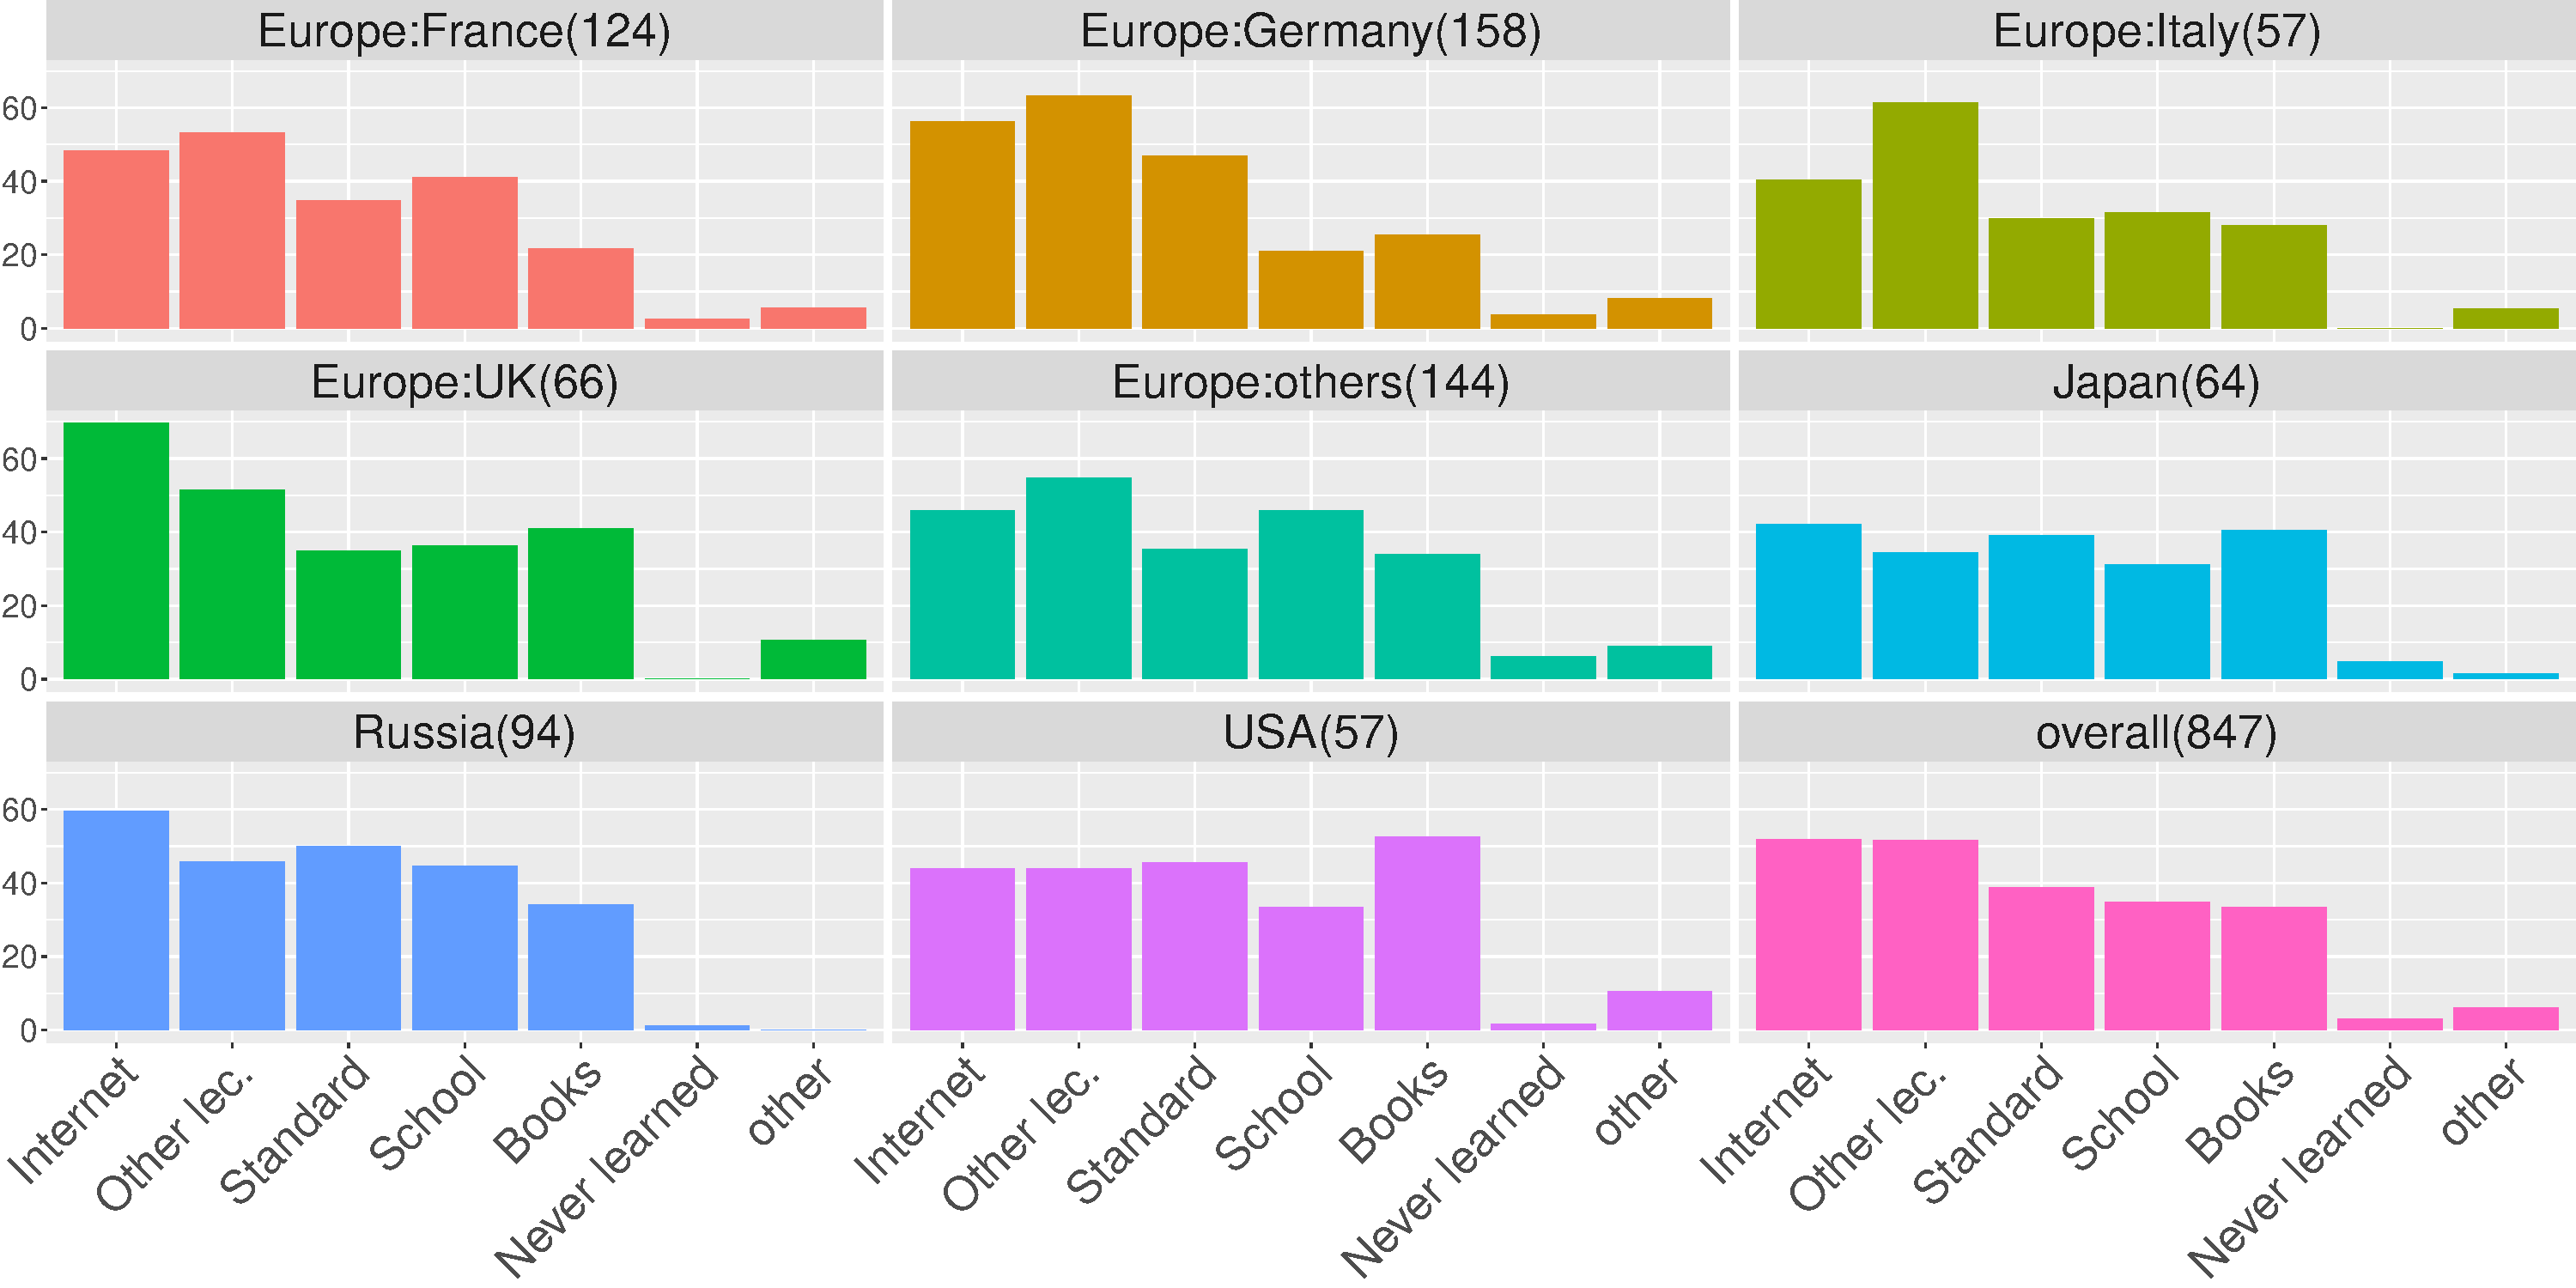
\includegraphics[width=8.0cm]{R-scripts/Q10.pdf}
\vspace{-2mm}
\caption{Q10: Learning MPI {\it(multiple)}}
\label{fig:learning-mpi}
\end{center}
\end{figure}

Fig.~\ref{fig:reading-standard} shows the familiarity of the participants with
the official MPI standard document (asking if participants have read the MPI
standard document). Not necessarily surprising, around 60\% of participants,
independent from \countries, have partially read the MPI standard. Interestingly
in UK, \revision{the percentage of participants having read the entirety of the MPI
standard is similar to the percentage of users having never read the
standard.}
{the percentage of participants having read the entirety of the MPI
standard and the percentage of users having never read the
standard are the highest among the \mcountries.}
\revision{In}{At the} same time, UK participants overwhelmingly learned MPI from online sources,
which usually \revision{translate by}{translates to} via practical examples.

\begin{figure}[tb]
\begin{center}
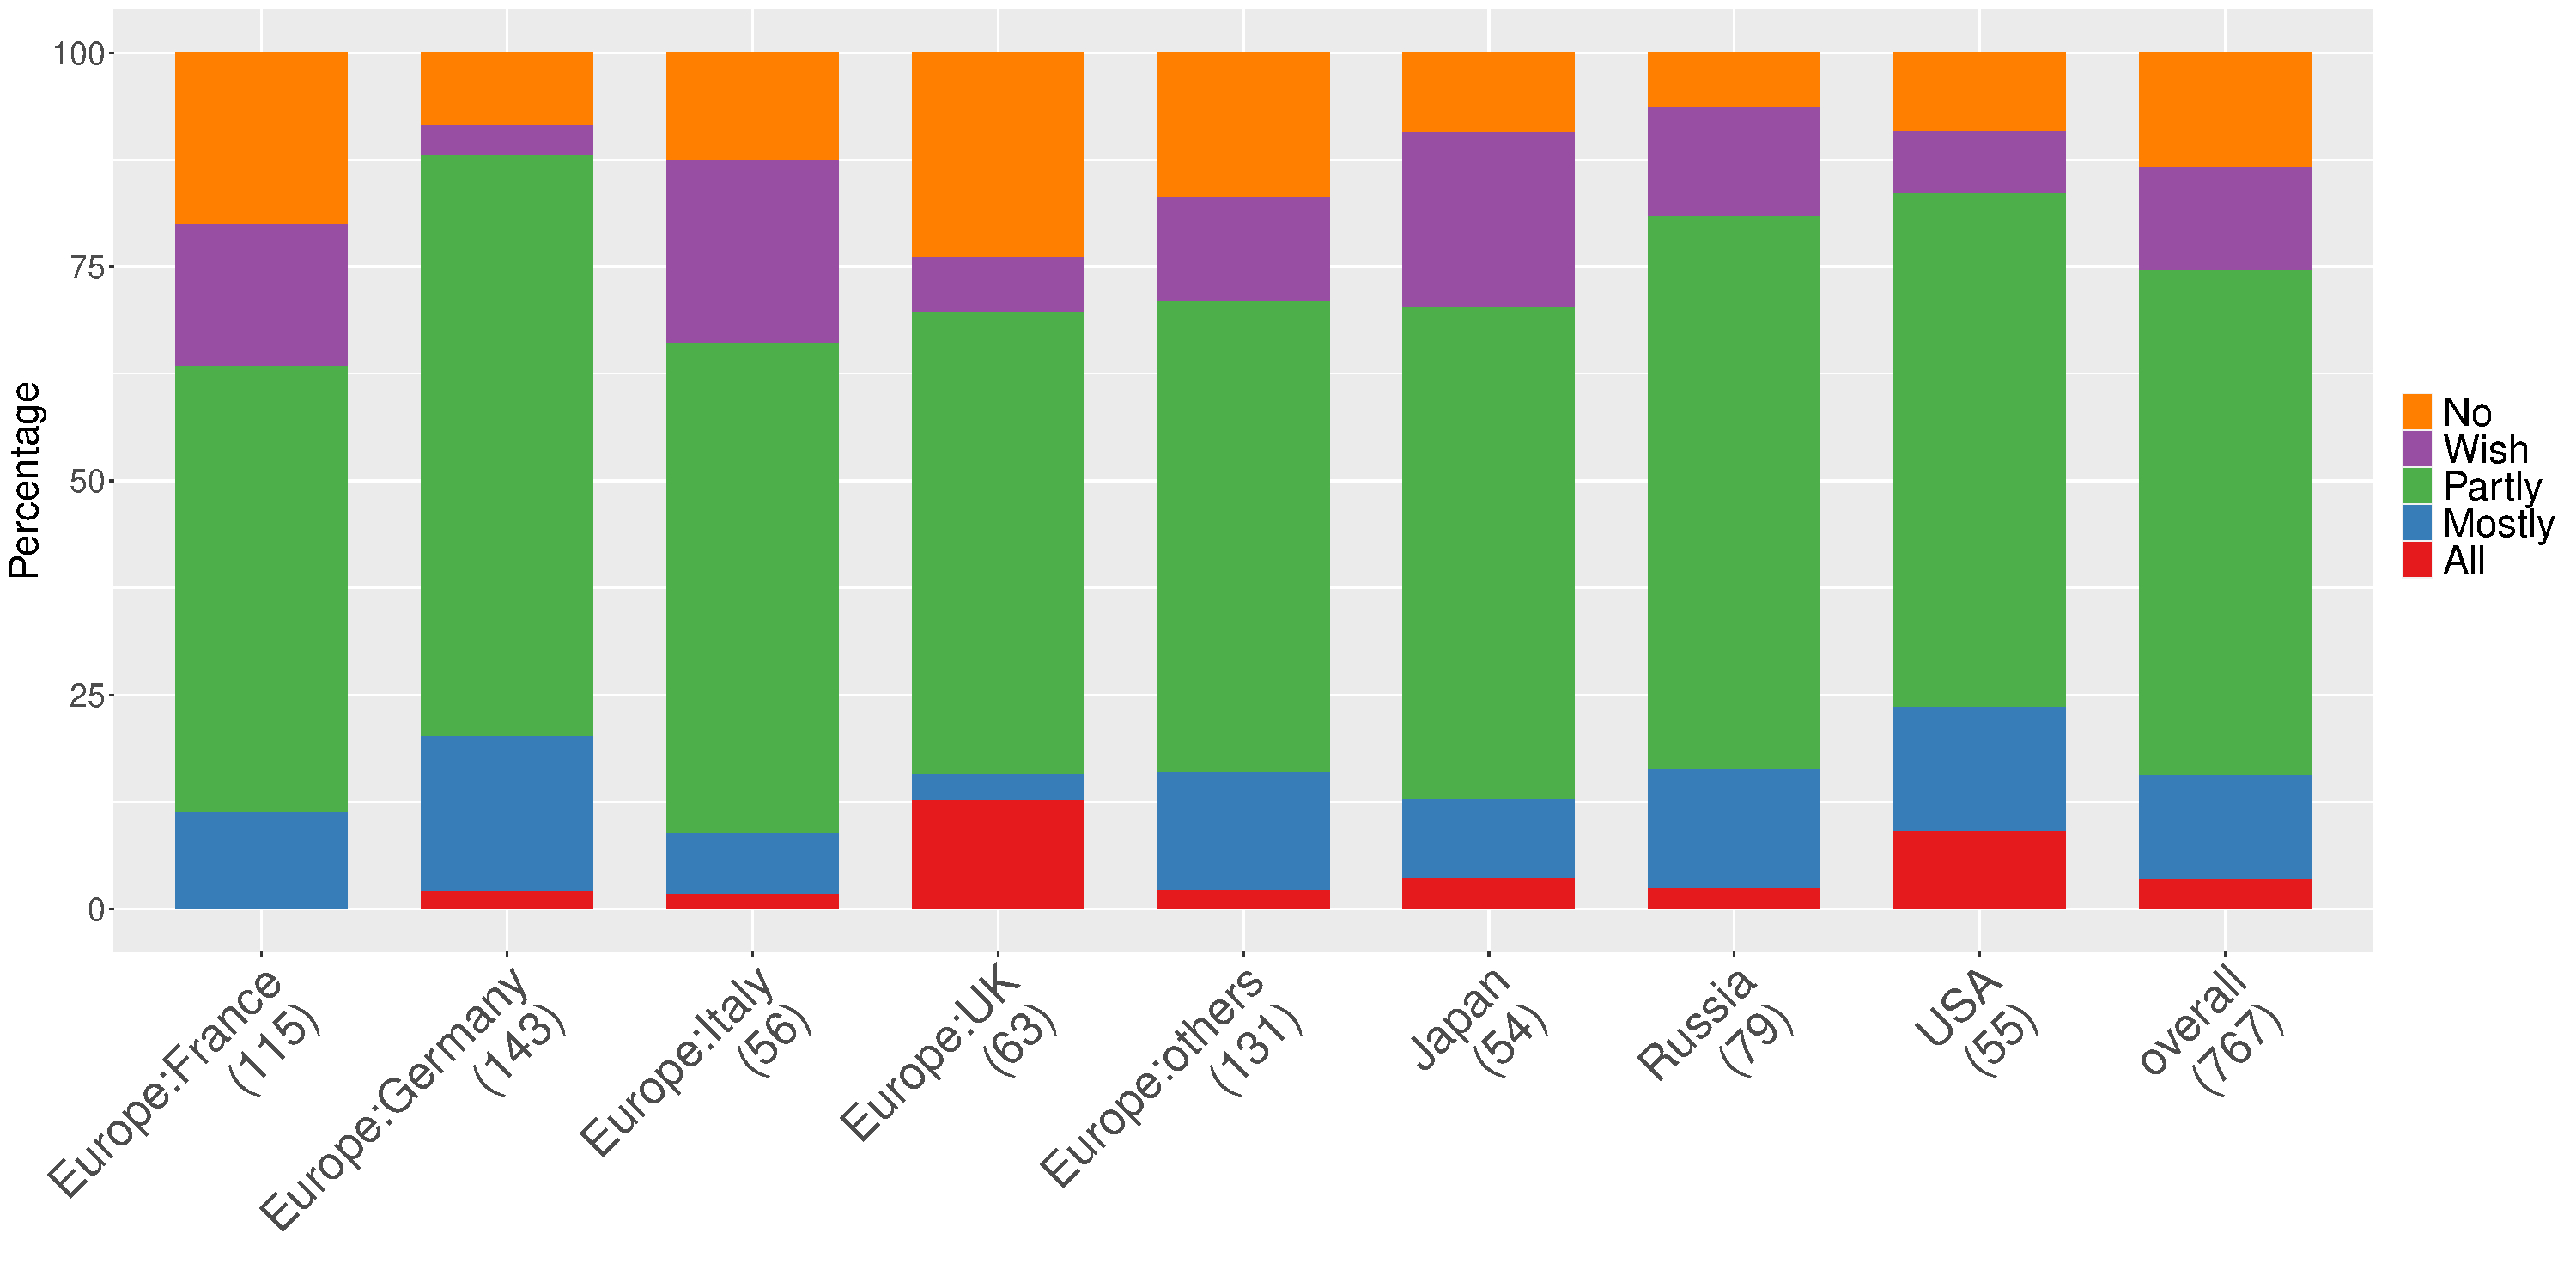
\includegraphics[width=8.0cm]{R-scripts/Q9.pdf}
\vspace{-2mm}
\caption{Q9: Reading MPI Standard {\it(single)}}
\label{fig:reading-standard}
\end{center}
\end{figure}

While the MPI standard is certainly not the best document for learning MPI, it
is the most valid and trusted source for checking the specification of the MPI
API. Fig.~\ref{fig:checking-spec} shows the percentages of Q14 asking
\myquote{How do you check MPI specifications when your are writing MPI
programs?} Most users are checking MPI specifications by reading online
documentations (e.g., man pages), searching Internet, and reading the standard.
As shown in the previous figure (Fig.~\ref{fig:reading-standard}), users are
reading the standard partly because of checking the MPI specifications.

\begin{figure}[tb]
\begin{center}
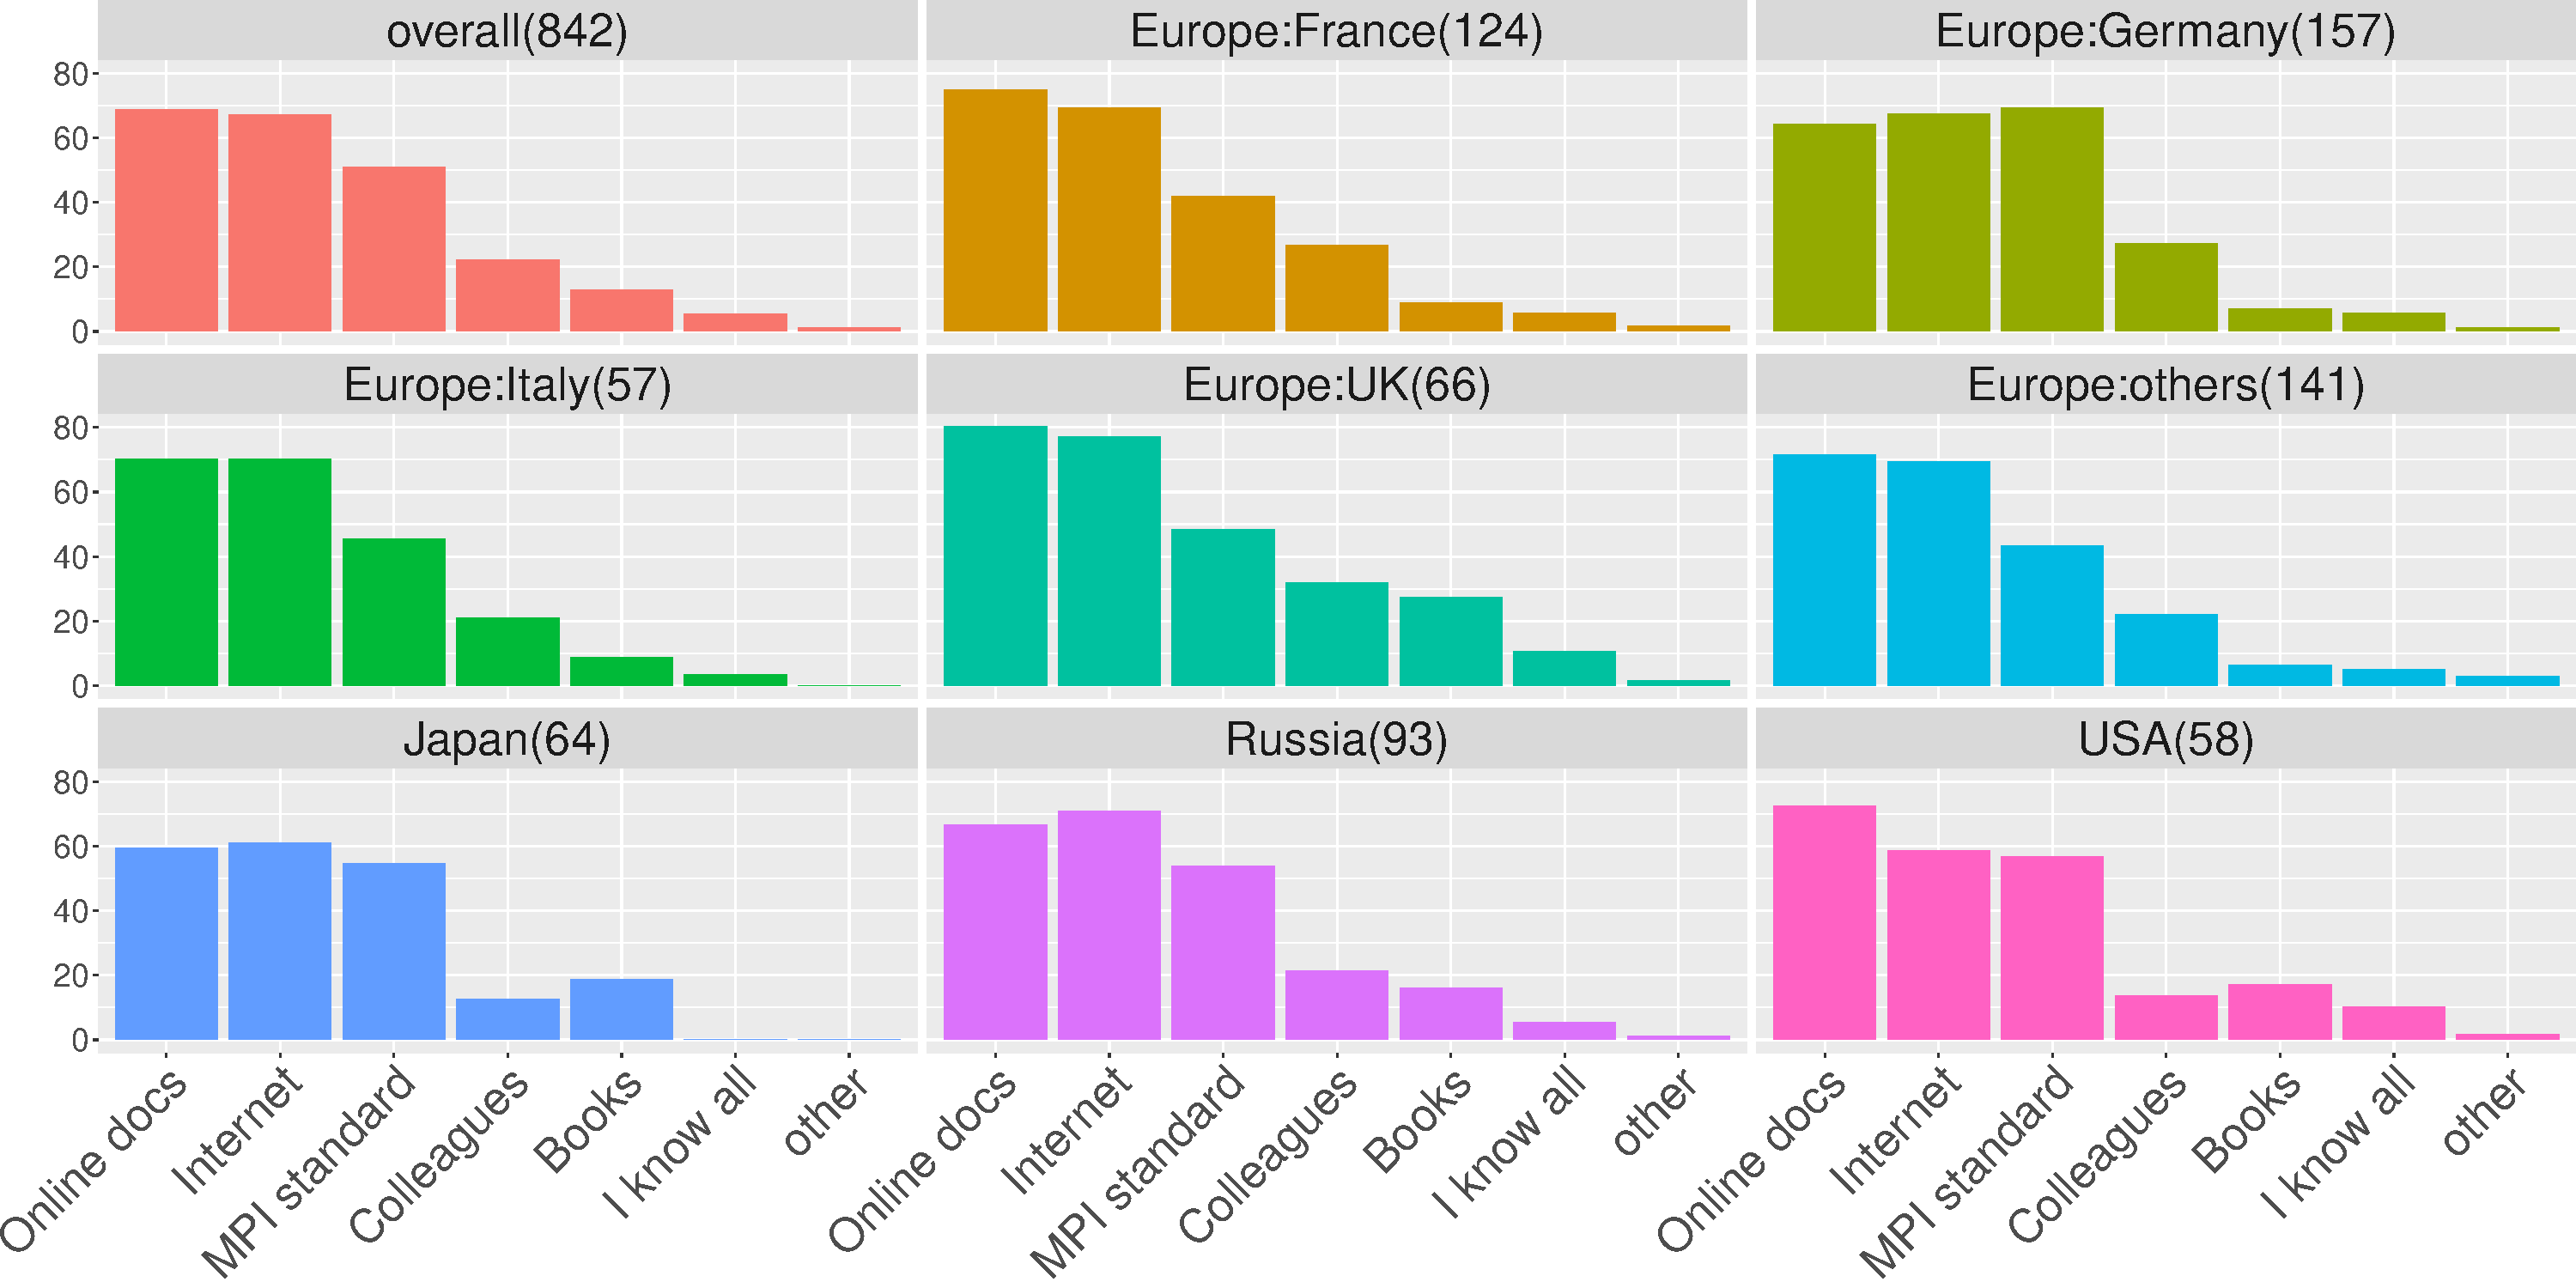
\includegraphics[width=8.0cm]{R-scripts/Q14.pdf}
\vspace{-2mm}
\caption{Q14: Checking Specification {\it(multiple)}}
\label{fig:checking-spec}
\end{center}
\end{figure}

It would have been interesting to have the cross-tab analysis between Q3 (MPI
skill) and Q9 (reading MPI standard). Unfortunately the participants reading the
standard partly dominates and the cross-tab analysis would not give us any clear
evidence.
%
Instead Fig.~\ref{fig:reading-standard-and-checking-spec} presents a cross-tab
analysis between Q3 and Q14. There can be seen a weak correlation, those who
\revision{check more regularly the MPI standard}{check the MPI
  standard more regularly} have higher MPI skill, in some
\mcountries\  (France, Germany, and Japan).

\begin{figure}[tb]
\begin{center}
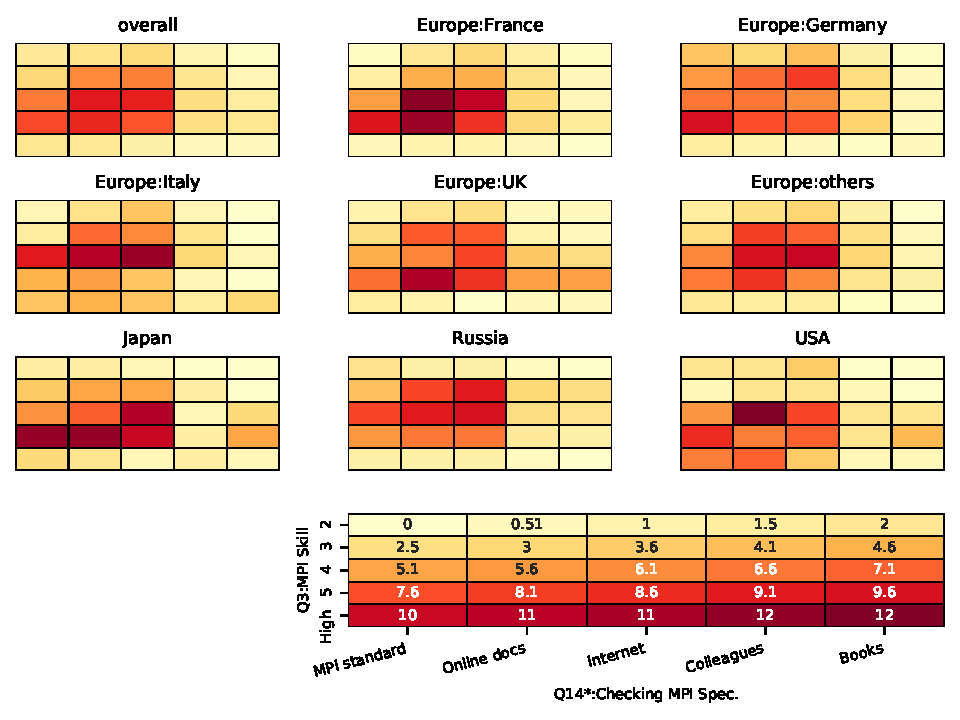
\includegraphics[width=8.0cm]{Figs/Q3-Q14.pdf}
\caption{Q3-Q14: MPI Skill {\it(single)} and regular checking of the MPI Specification {\it(single)}}
\label{fig:reading-standard-and-checking-spec}
\end{center}
\end{figure}

Another interesting result can be seen in Fig.~\ref{fig:prog-skill} asking
\myquote{Rate your overall programming skill (non-MPI programs)}. People who
auto-evaluate  high their programming skills (\revision{basically }{}those who chose 4 or
more on the skills grade) account for more than 90\%. This indicates that MPI
users are seasoned developers, or at least programmers with high programming
skills. This might indicate that MPI programming requires specific skills whom
basic developers do not necessarily master, or that before starting to write
parallel applications (where MPI is necessary) most developers have already
become acquainted with programming. By \country\ comparison, Russia shows a
different tendency from other \countries.

\begin{figure}[tb]
\begin{center}
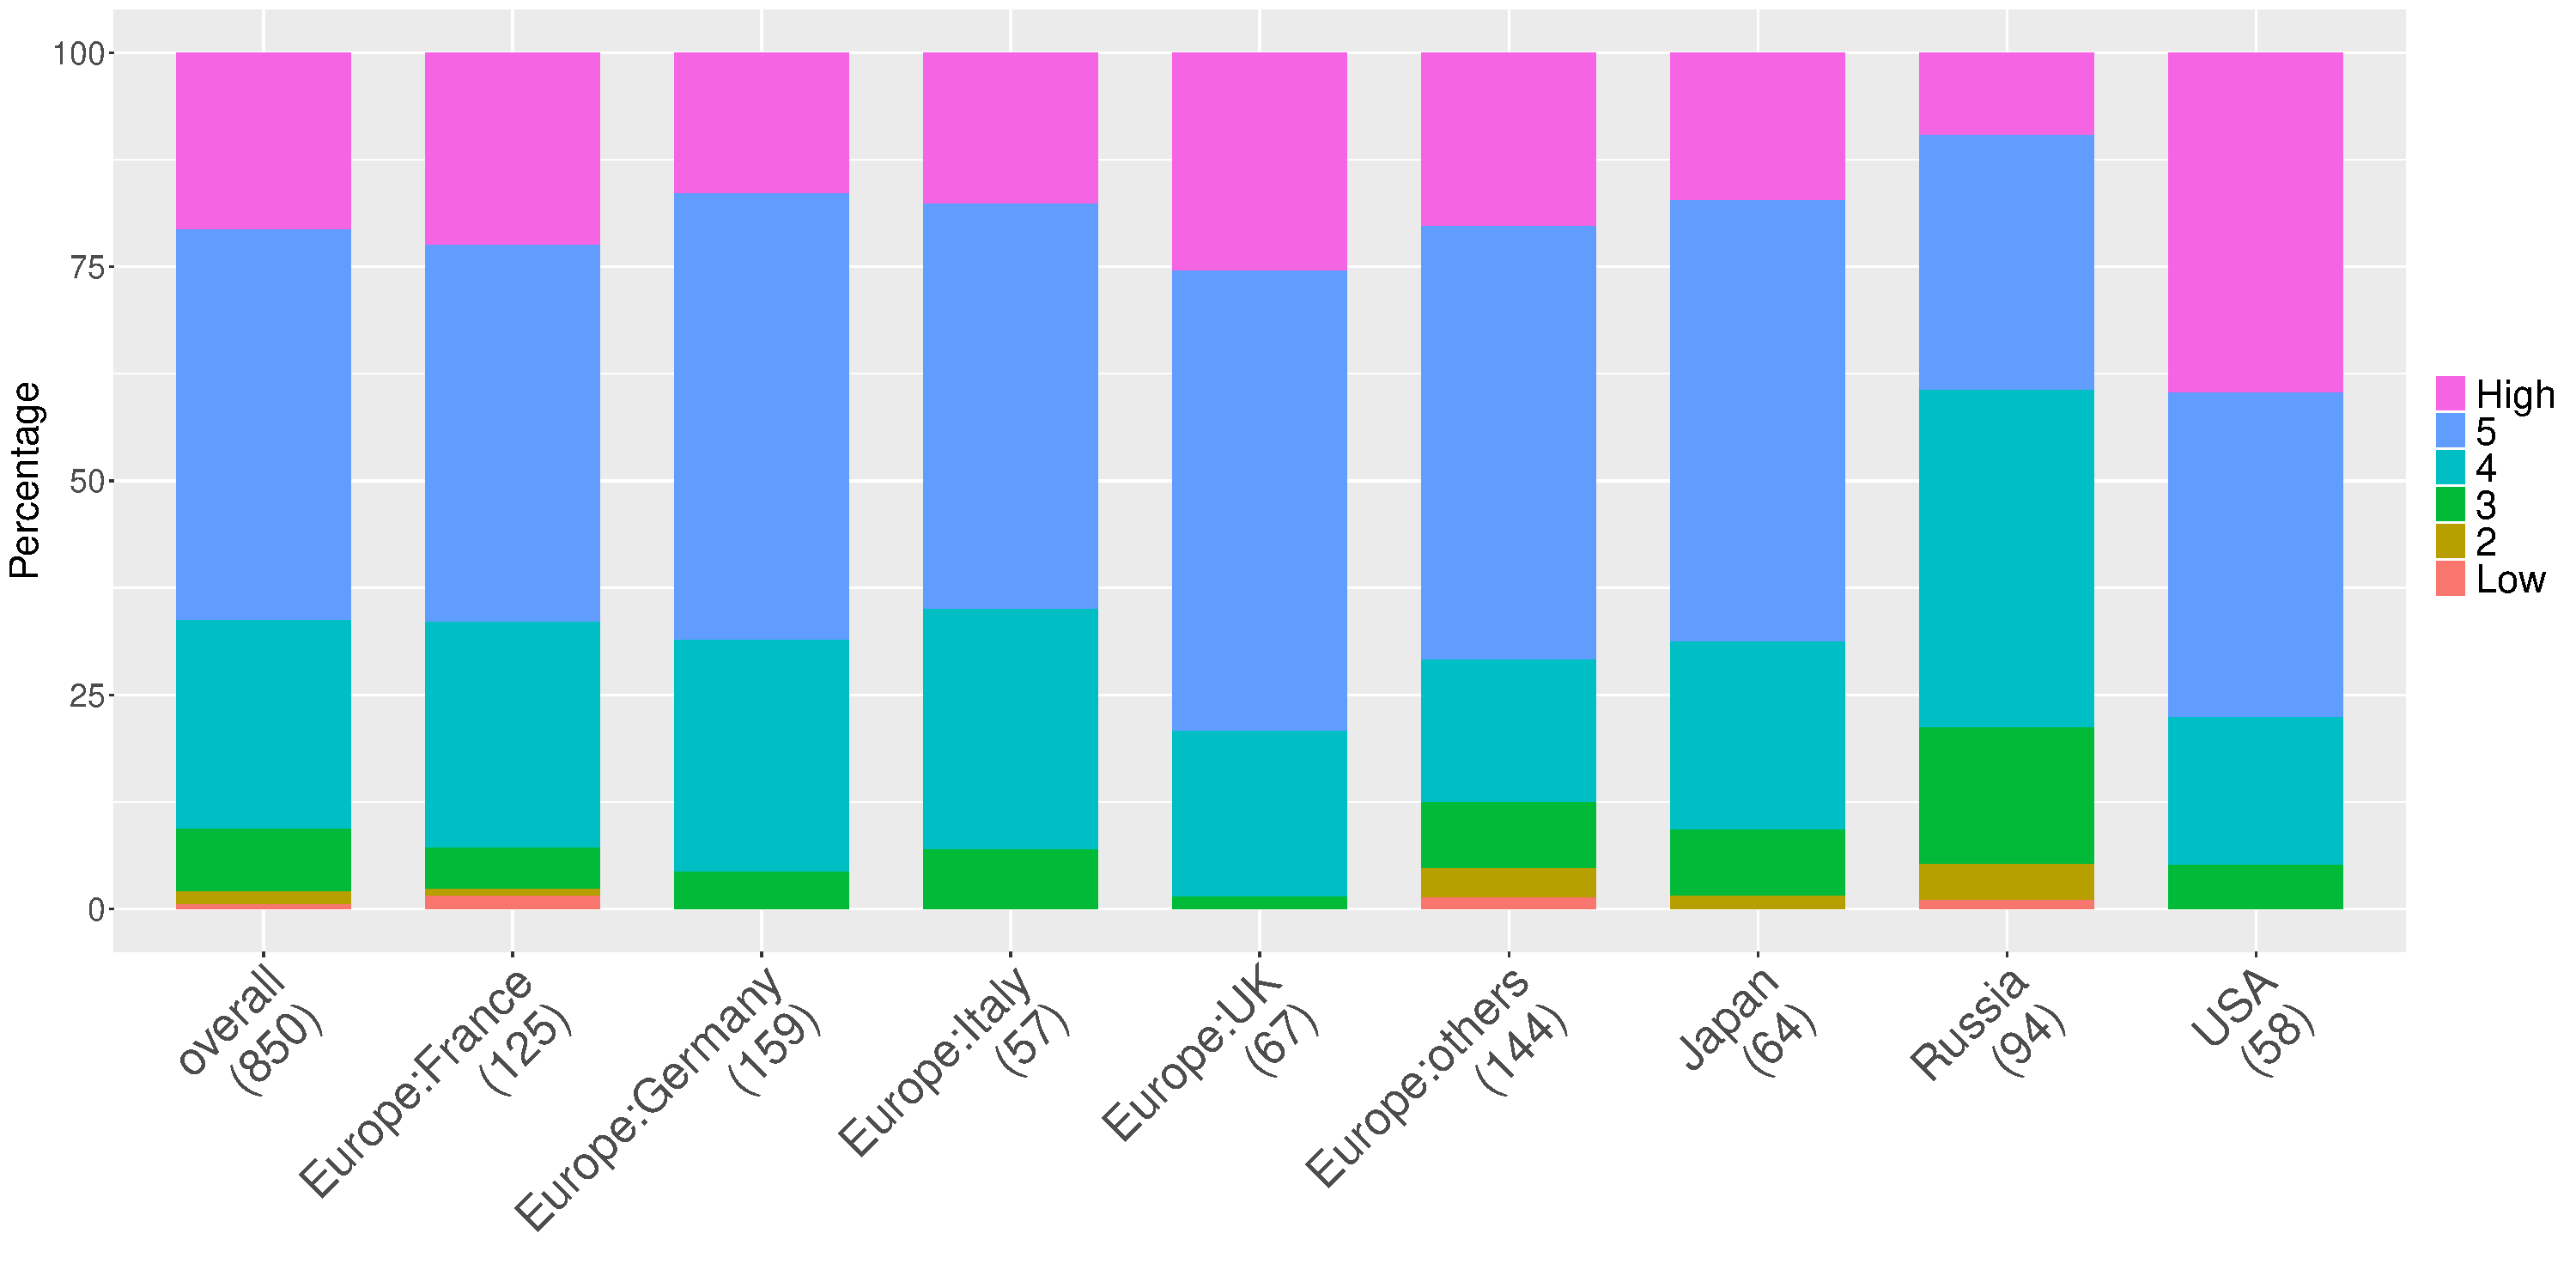
\includegraphics[width=8.0cm]{Figs/Q2.pdf}
\caption{Q2: Rate your overall programming skill (non-MPI
  programs)}
\label{fig:prog-skill}
\end{center}
\end{figure}

\begin{figure}[tb]
\begin{center}
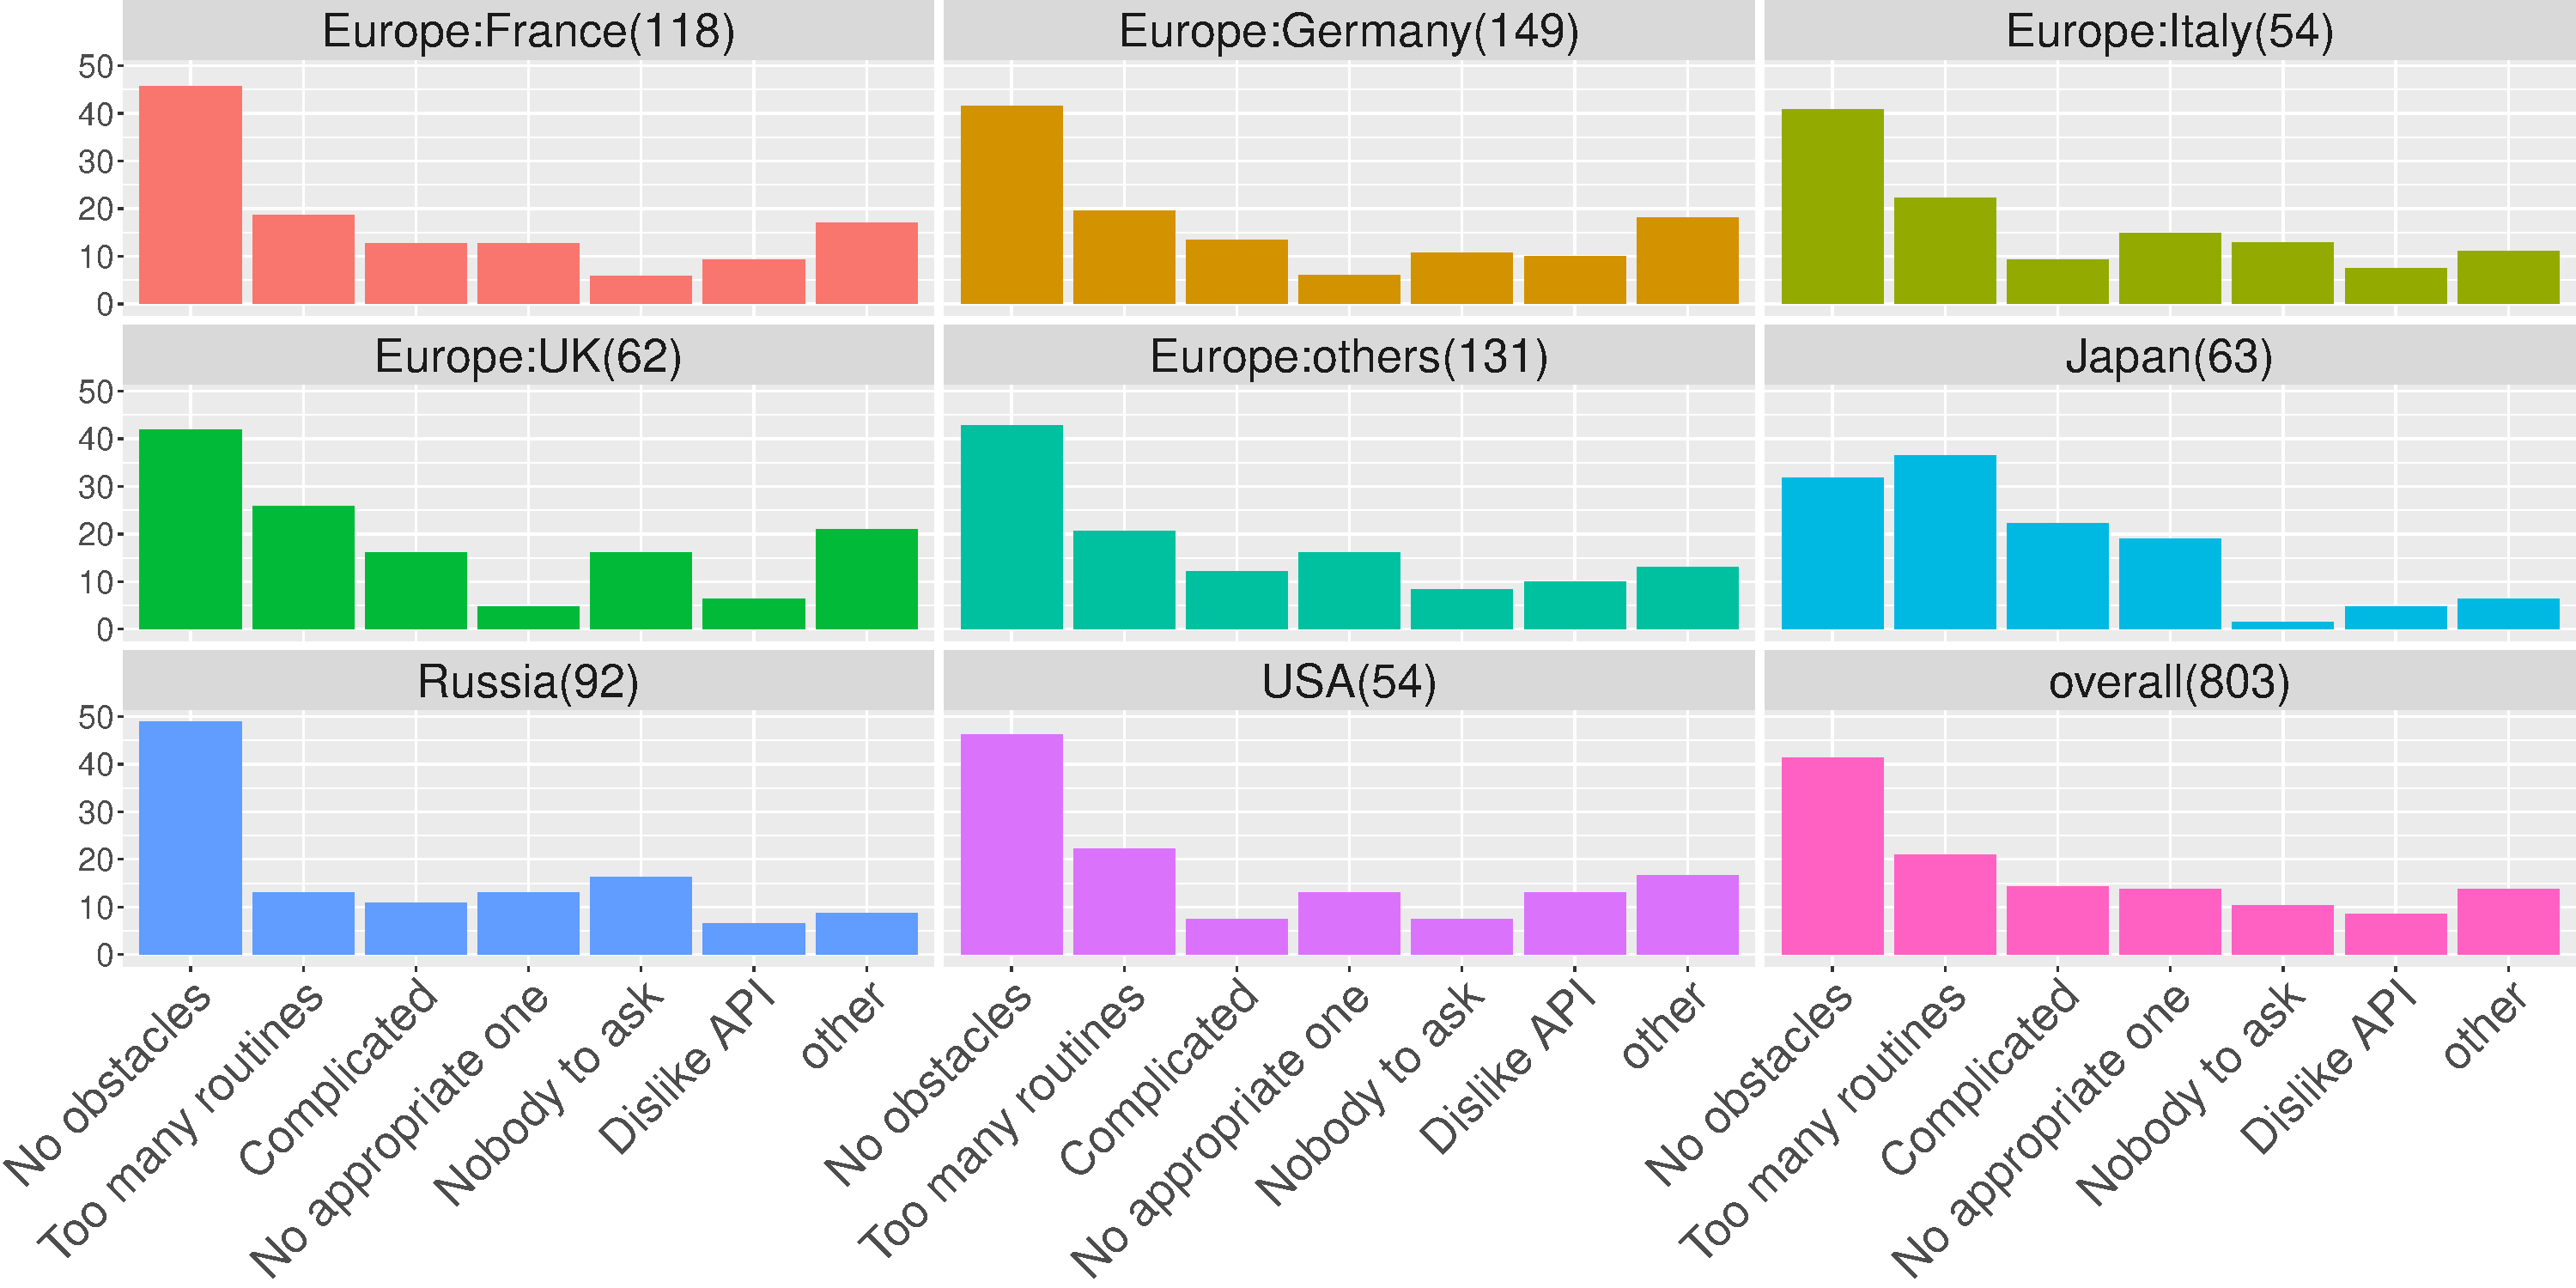
\includegraphics[width=8.0cm]{R-scripts/Q19.pdf}
\caption{Q19: Learning Obstacles {\it(multiple)}}
\label{fig:learning-obstacles}
\end{center}
\end{figure}

\begin{figure}[tb]
\begin{center}
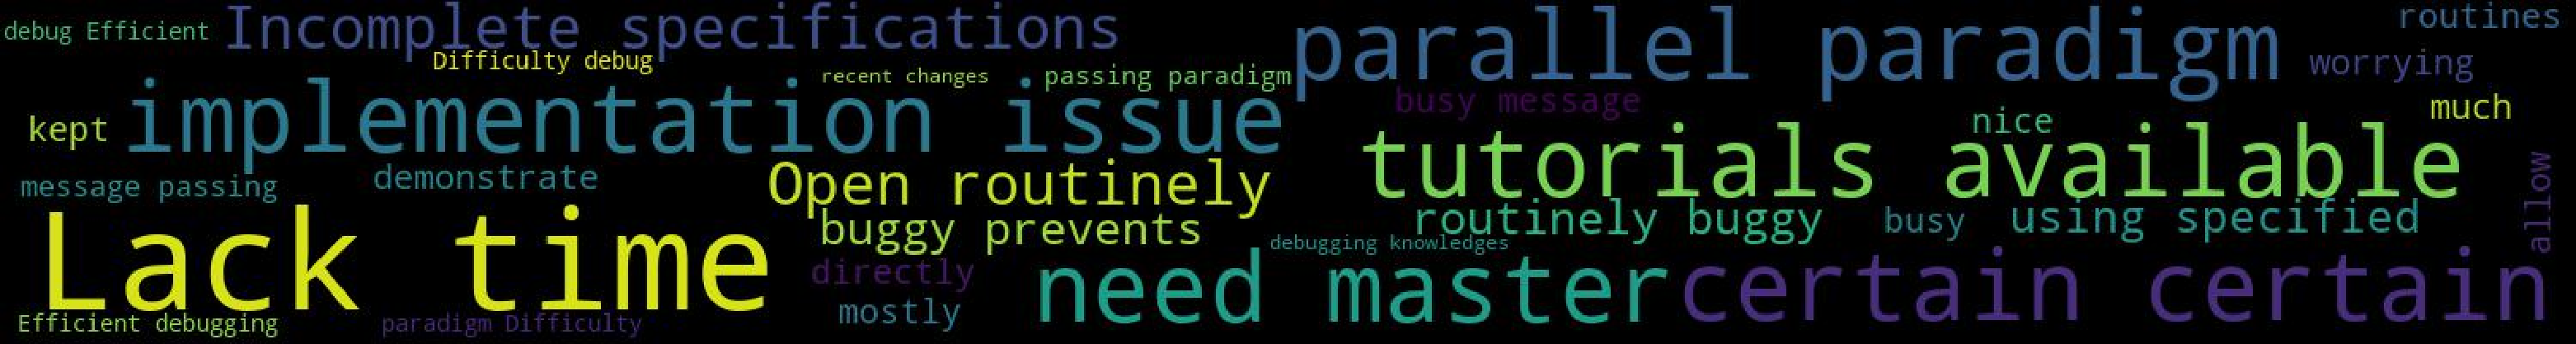
\includegraphics[width=8.0cm]{Figs/Q19-others.pdf}
\caption{Q19: Learning Obstacles - Text mining (WordCloud)}
\label{fig:learning-obstacles-wc}
\end{center}
\end{figure}

Generally speaking, allowing participants to freely answer questions in text
boxes \revision{lead}{leads} to a large variety of disparate answers, making difficult to find
commonality between mostly subjective answers and to put forward a consistent
answer. Despite this, we had one particular question in our survey, where we
felt that predefined answers would have \revision{been}{} led to unsatisfactory results, and
where more diverse information could be gathered with a combination of
preselected answers and the opportunity to enter a different answer in a text
box. This particular question, Q19, relates to \myquote{What are your obstacles
to mastering MPI}, and is represented in Fig.~\ref{fig:learning-obstacles}.
% there can be a case where a particular question in a survey may ignite for
% participants to explode their dissatisfaction by writing messages into a free
% text field. \comment{In our survey Q19 is such a question.} The largest number
% of \myquote{other} inputs in our survey can be found at Q19 asking
% \myquote{What are your obstacles to mastering MPI?}
% (Fig.~\ref{fig:learning-obstacles}).
Although the largest answer was one of the provided choices, \myquote{No
obstacles,} we got an exceptional 111 \myquote{other} inputs.
% Q4 and Q7 are the second largest (70), but these are because of the variety of
% answers.
\revision{
After post-analysis, we can report that out of these, 
more than 20 participants, 18\%, answered pinpointing
to how time consuming mastering MPI is. Many other
participants pointed out the need for more clear MPI programming guideline
(\myquote{clear doc.}, \myquote{internal doc.}, \myquote{implementation doc.},
\myquote{performance guideline}, and so on, in their words). Some participants
\revision{complaints}{complaint} about MPI implementations and the (performance or specification)
differences among implementations.}
{
  Fig.~\ref{fig:learning-obstacles-wc} shows the text mining result of
  the free text inputs (using WordCloud\cite{wordcloud}, \footnote{WordCloud parameters: \tt
    min\_word\_length=4, collocations=True,
    collocation\_threshold=5,
    max\_words=30}. As shown, \myquote{lack
  (of) time} is highlighted.
}

\begin{figure}[tb]
\begin{center}
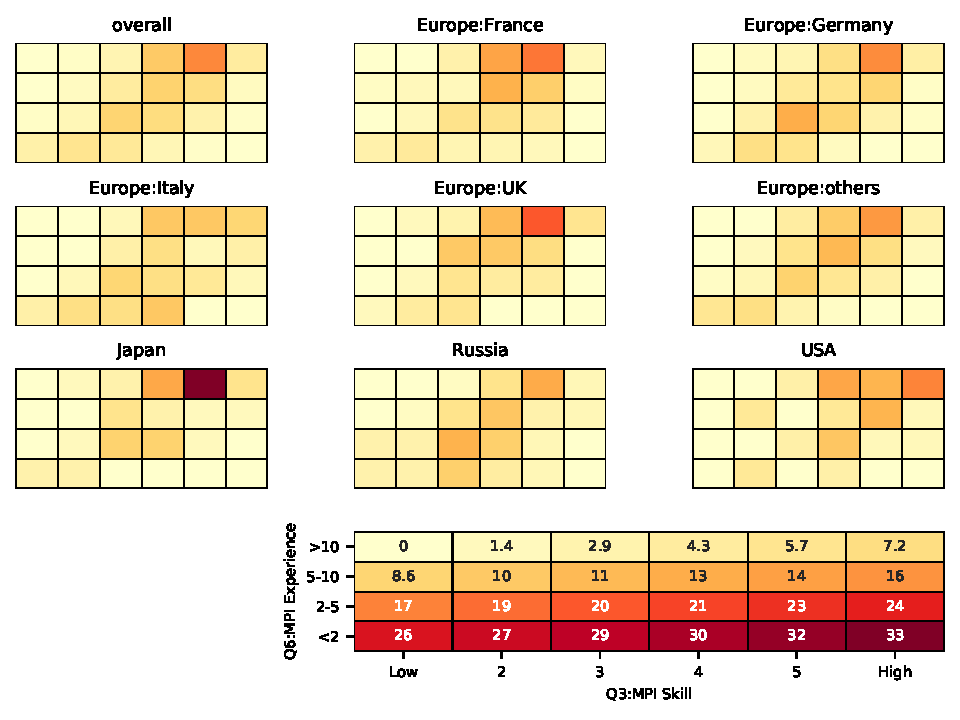
\includegraphics[width=8.0cm]{Figs/Q6-Q3.pdf}
\caption{Q6-Q3: MPI Experience {\it(single)} and MPI Skill {\it single}}
\label{fig:experience-and-skill}
\end{center}
\end{figure}

As shown in Fig.~\ref{fig:experience-and-skill}, the cross-tab heatmap graphs
between Q6 (Fig.~\ref{fig:mpi-experience}) and Q3 \revision{(Fig.~\ref{fig:mpi-skill}),}{(Fig.~\ref{fig:mpi-skill})}
highlight a strong correlation, from lower-left to higher-right, between those
two questions regardless of \mcountries. In fact, these graphs confirm a prior
answer regarding mastering MPI, indicating that it takes more than somewhere
between 5 and 10 years of MPI programming experience to reach a high MPI skill
(\myquote{4} to \myquote{High}). The answer is confirmed across the entire
spectrum and in most \mcountries.
% Many MPI users in US consider that the high (\myquote{4} or higher) MPI skill
% can be reached in 5 to 10 years. Hence, it takes more than 5 or 10 years to
% reach the high MPI skill mostly.
Considering this fact and the nature and size of the MPI specification
(Subsection~\ref{sec:mpi-aspects}), it is apparent that there is a, widely
spread, belief that MPI could be said to be very difficult specification to
master, and that the standardization body would need to put forward some serious
efforts to facilitate the adoption and help MPI become more mainstream.

\subsection{MPI Programming Difficulty and Tuning}

Fig.~\ref{fig:difficulty} shows the result of Q15 asking \myquote{What is the
most difficult part of writing an MPI program?} and
Fig~\ref{fig:tuning} shows the result of Q23 asking \myquote{Is there any
room for performance tuning in your MPI programs?} The largest part
of US and UK participants chose \myquote{algorithm design} whilst the
participants of the other \countries\  chose
\myquote{Debugging}. In US, the second largest choice was
\myquote{Domain Decomposition}. In Japan, the second largest is
\myquote{Tuning}.

\begin{figure}[tb]
\begin{center}
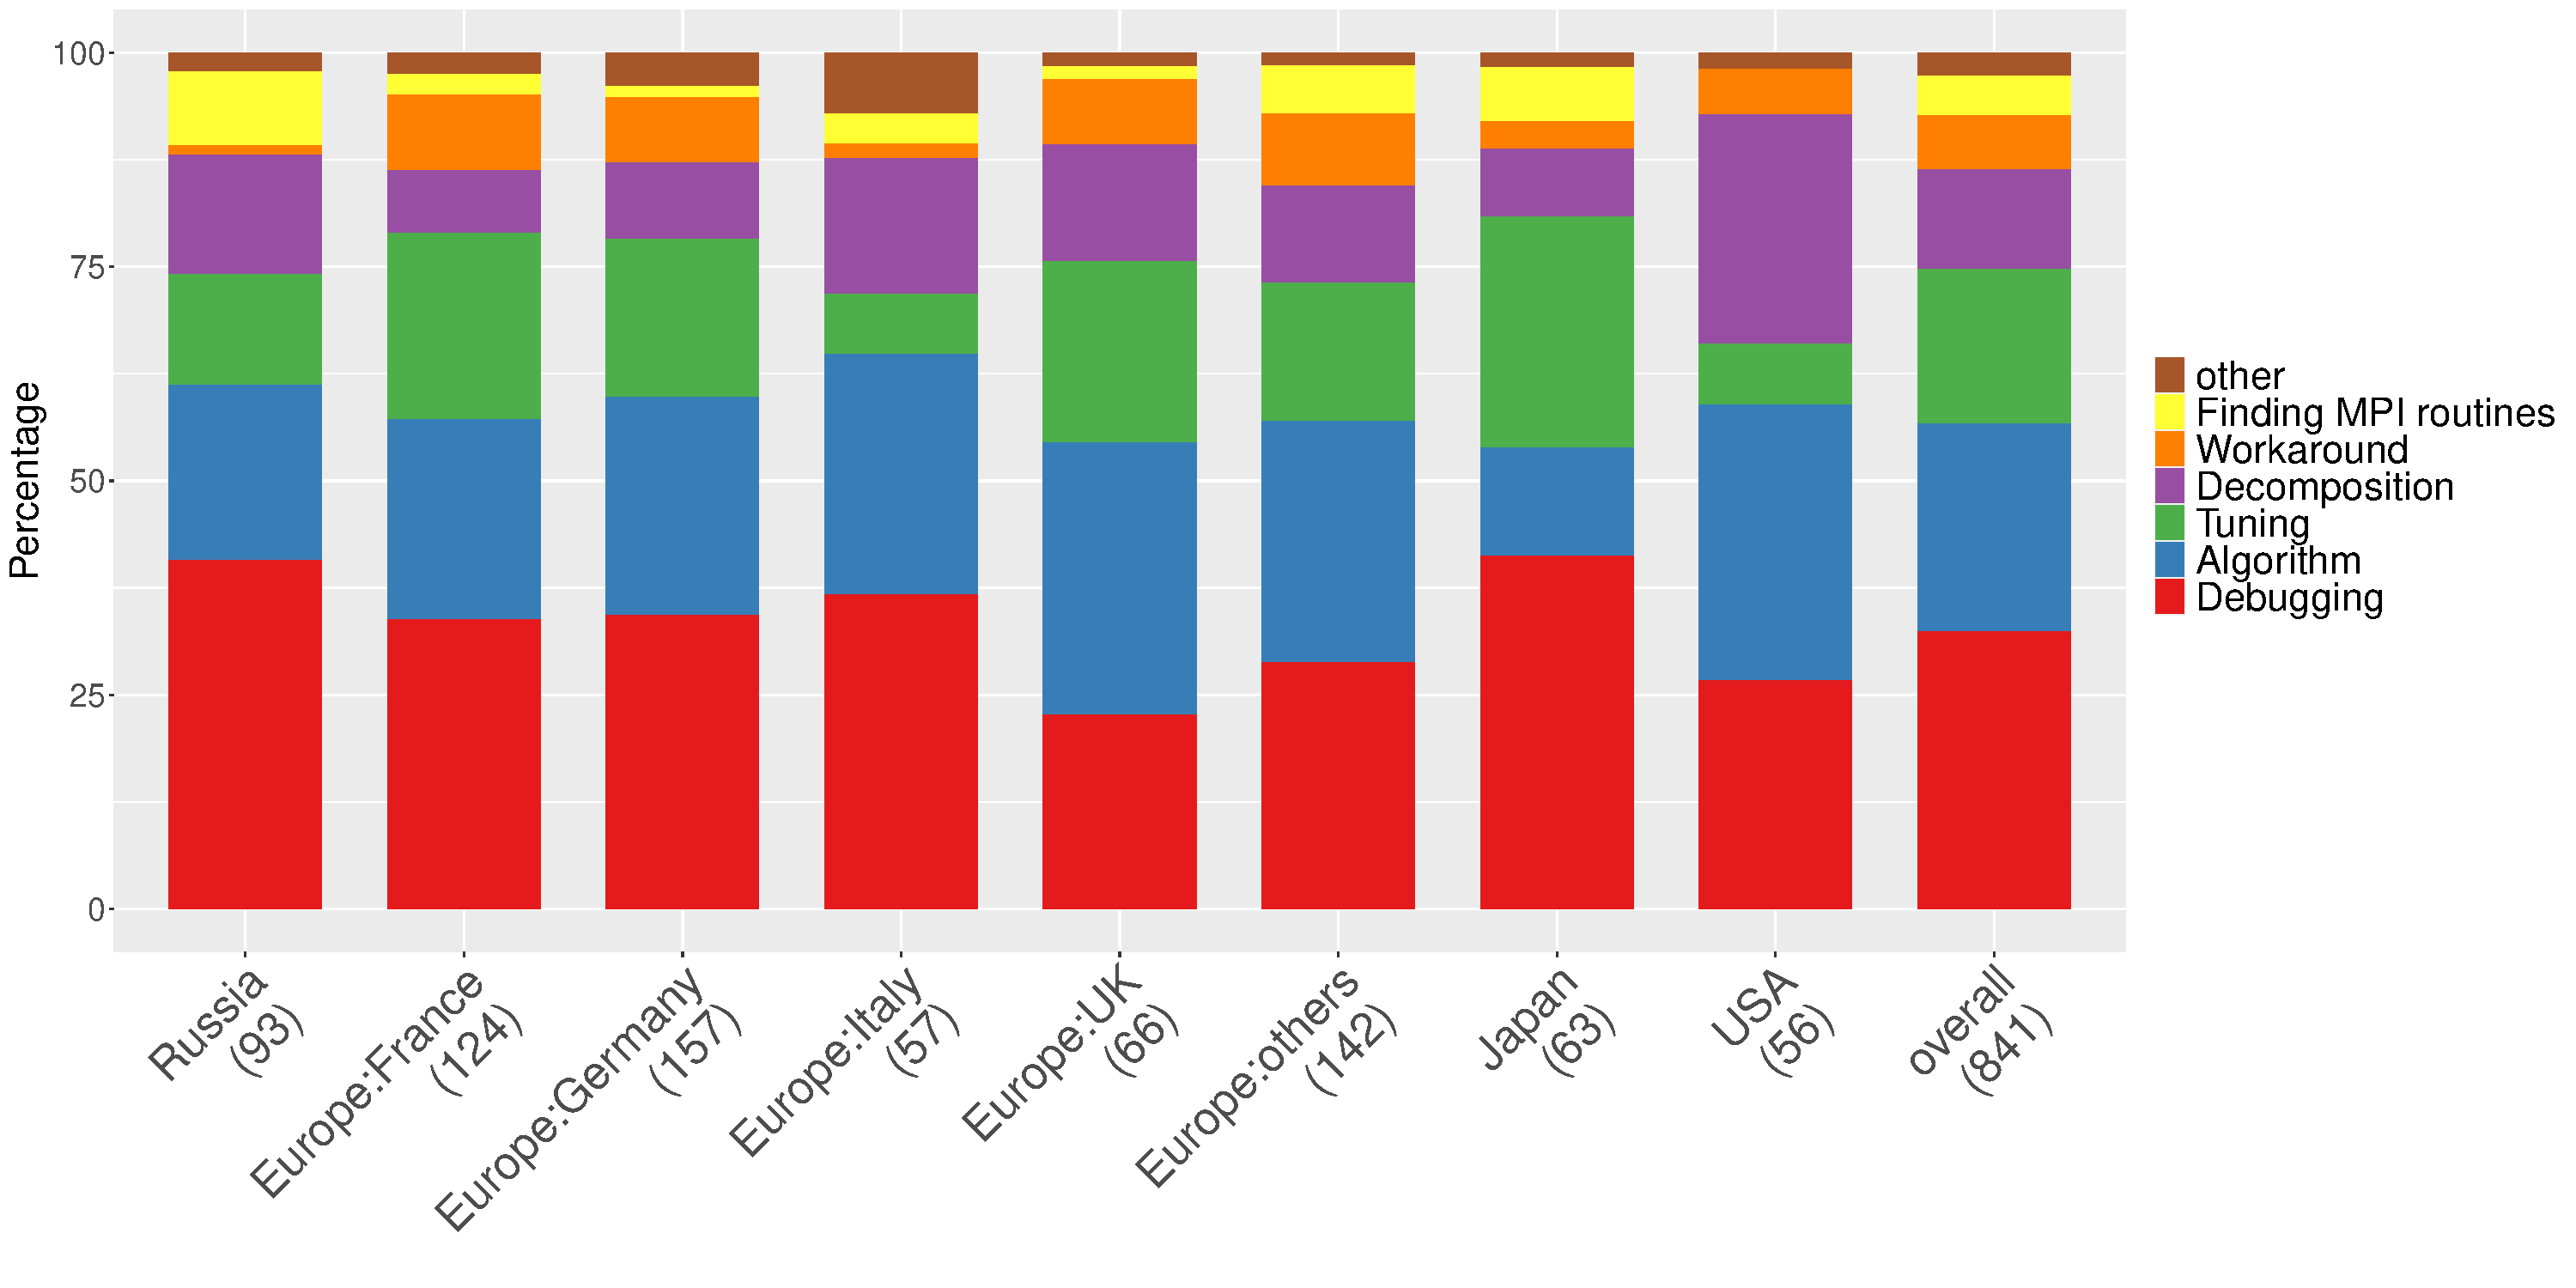
\includegraphics[width=8.0cm]{R-scripts/Q15.pdf}
\vspace{-2mm}
\caption{Q15: MPI Programming Difficulty {\it(single)}}
\label{fig:difficulty}
\end{center}
\end{figure}

Fig.~\ref{fig:tuning} has more divergence than Fig~\ref{fig:difficulty}. The
participants having selected \myquote{my MPI programs are well-tuned} account
for only around 10\%, with the exception of Japan and Russia. There seems to be
\revision{a lots of room to tune}{lots of potential for tuning} MPI programs in general, however, around 40\% of
participants said they do not have the necessary resources to do that. In Japan,
the percentage of well-tuned program is only few percent, highlighting the fact
that as parallel machines become more complex, users are feeling that an
increasing percentage of performance \revision{become}{becomes} unobtainable.
% Contrastingly, Russian percentage of choosing \myquote{well-tuned} is the
% highest among the \countries.

\begin{figure}[tb]
\begin{center}
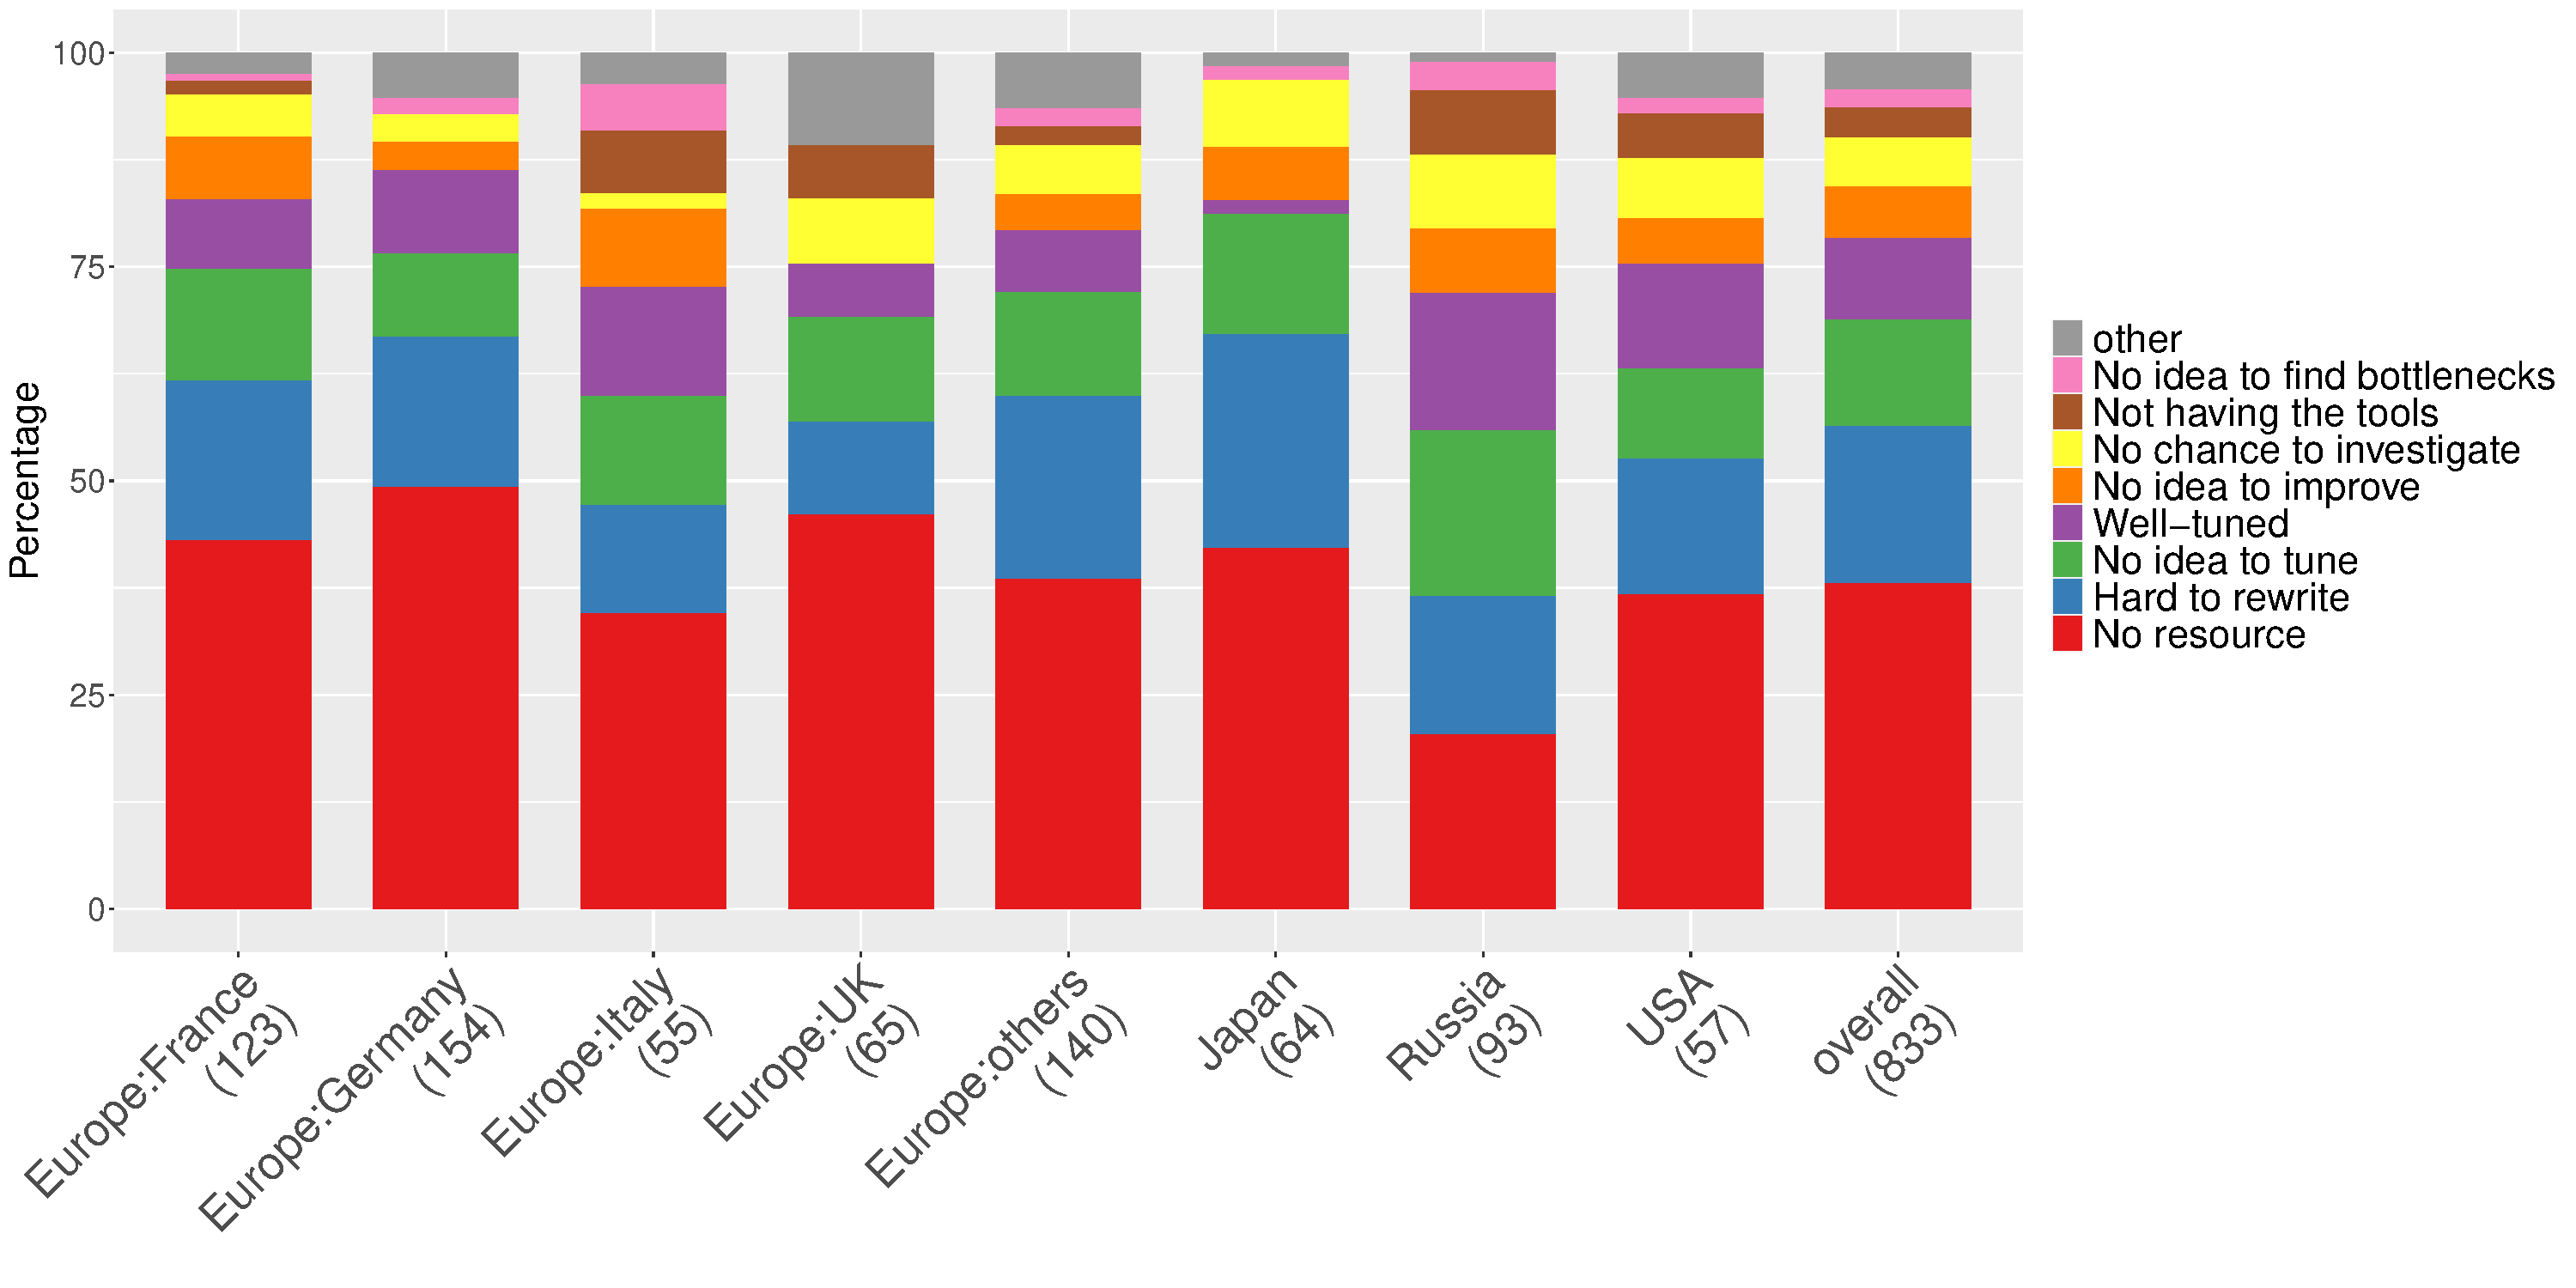
\includegraphics[width=8.0cm]{R-scripts/Q23.pdf}
\vspace{-2mm}
\caption{Q23: Performance Tuning {\it(single)}}
\label{fig:tuning}
\end{center}
\end{figure}

\subsection{Missing Features and Semantics}

It is a general concern how MPI provides optimization
opportunities in terms of hardware capabilities such as being able to
handle the various topologies of hardware components more
efficiently. To answer this, Q25 asked \myquote{If there were one
communication aspect which is not enough in the current MPI that could
improve the performance of your application, what would you
prioritize? Or $\ldots$} (Fig.~\ref{fig:missing-features}), and Q26 asking
\myquote{Is MPI providing all the communication semantics required by your
application? If not, what is missing?}
(Fig.~\ref{fig:missing-semantics}).

Fig.~\ref{fig:missing-features}, indicates that only 23\% of overall MPI users
are satisfied with the current situation. Interestingly enough the second
largest percentage is \myquote{Additional optimization opportunities in terms of
communication (network topology awareness, etc.)}, followed by
\myquote{Multi-thread} and \myquote{Optimization opportunities except
communication (architecture awareness, dynamic processing, accelerator support,
etc.)}.

\begin{figure}[tb]
\begin{center}
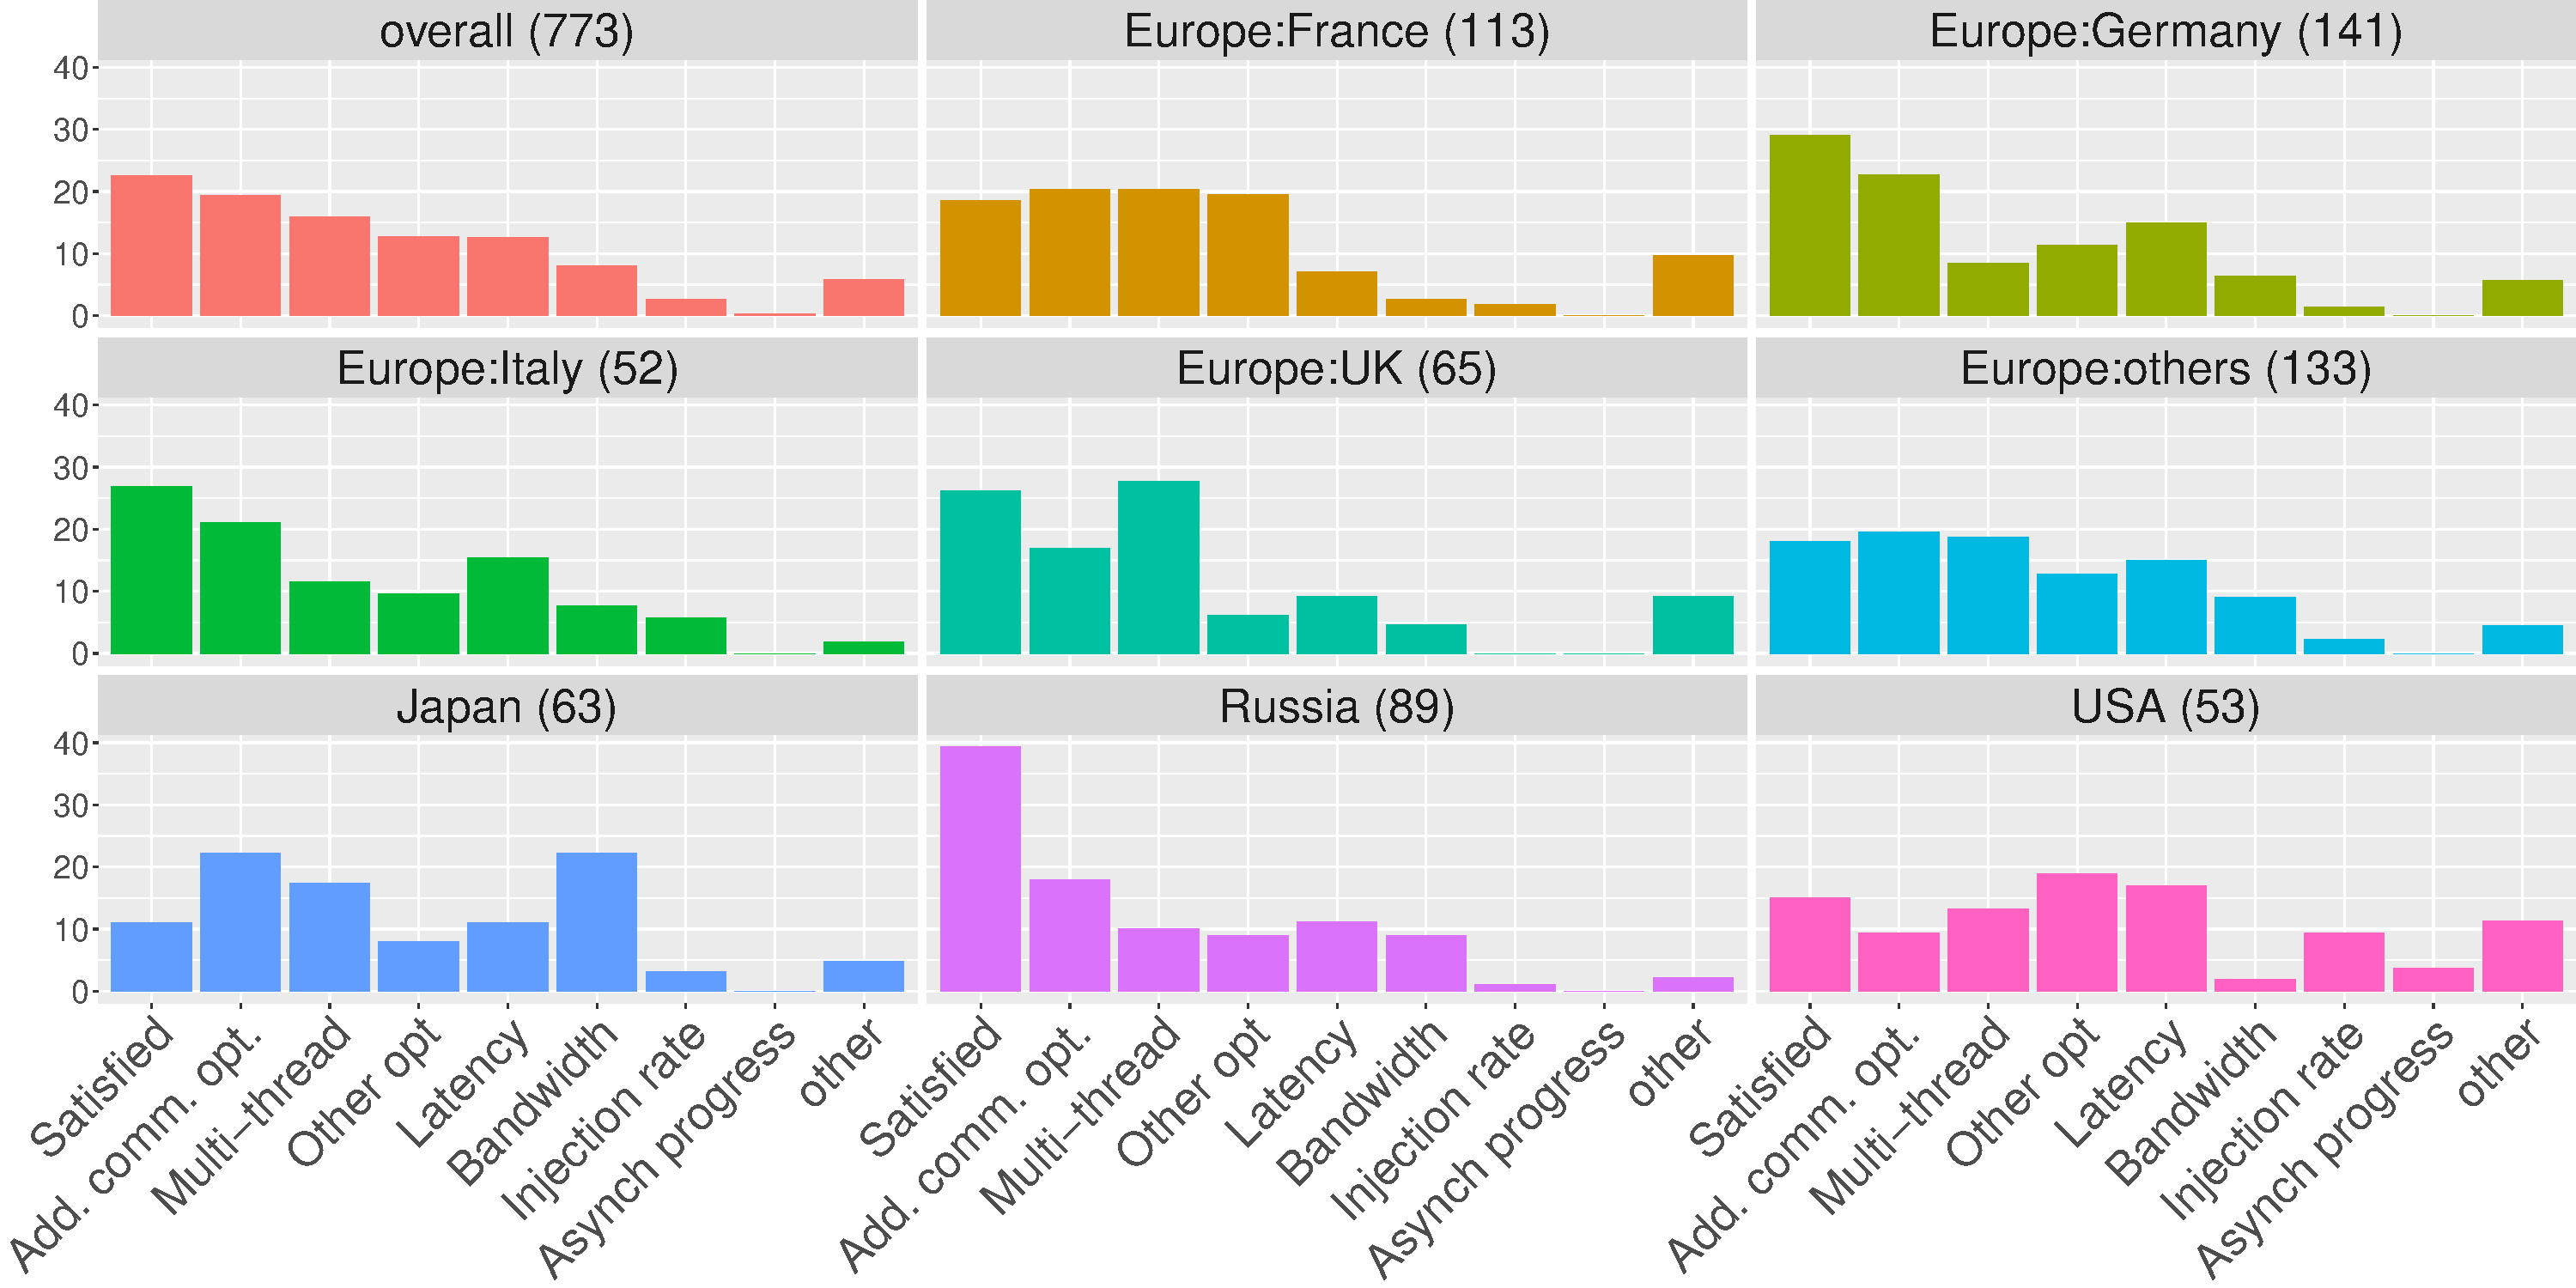
\includegraphics[width=8.0cm]{R-scripts/Q25.pdf}
\vspace{-2mm}
\caption{Q25: Features to improve {\it(single)}}
\label{fig:missing-features}
\end{center}
\end{figure}

Q26 is somewhat similar to Q25, but looking for more precise answers. This
question \revision{tackles}{addresses} the issue on which semantic features are missing from MPI.
Overall a very similar picture emerges with Q25, almost one third of the
participants are satisfied with the existing MPI features. There is a high
discrepancy between Japan, where users are the least satisfied with the current
situation, and Russia which hosts the most satisfied MPI users.
%
The situation here is similar to what we \revision{}{have} seen in Q25, with the highest answer
being \myquote{Additional optimization opportunities in terms of communication
(topology awareness, locality, etc.)}. Thus, it appears that efficiently
managing the topology and the locality seem a major concern to many users. Then
comes the concerns about the lack of resilience, a concern shared by more than
20\% of the participants. It is very interesting to note that most \mcountries\
have expressed concerns about resilience, but we do not have enough information
to understand the root cause. Hiding latency through generalization of
asynchrony over the whole set of functions is another point raised repeatedly.
16\% of the users think that a simpler and easier API would be desirable.
Although there are relatively big disparity in the satisfaction (answering
\myquote{MPI provides all}), the disparities of the other answers are smaller.

\begin{figure}[tb]
\begin{center}
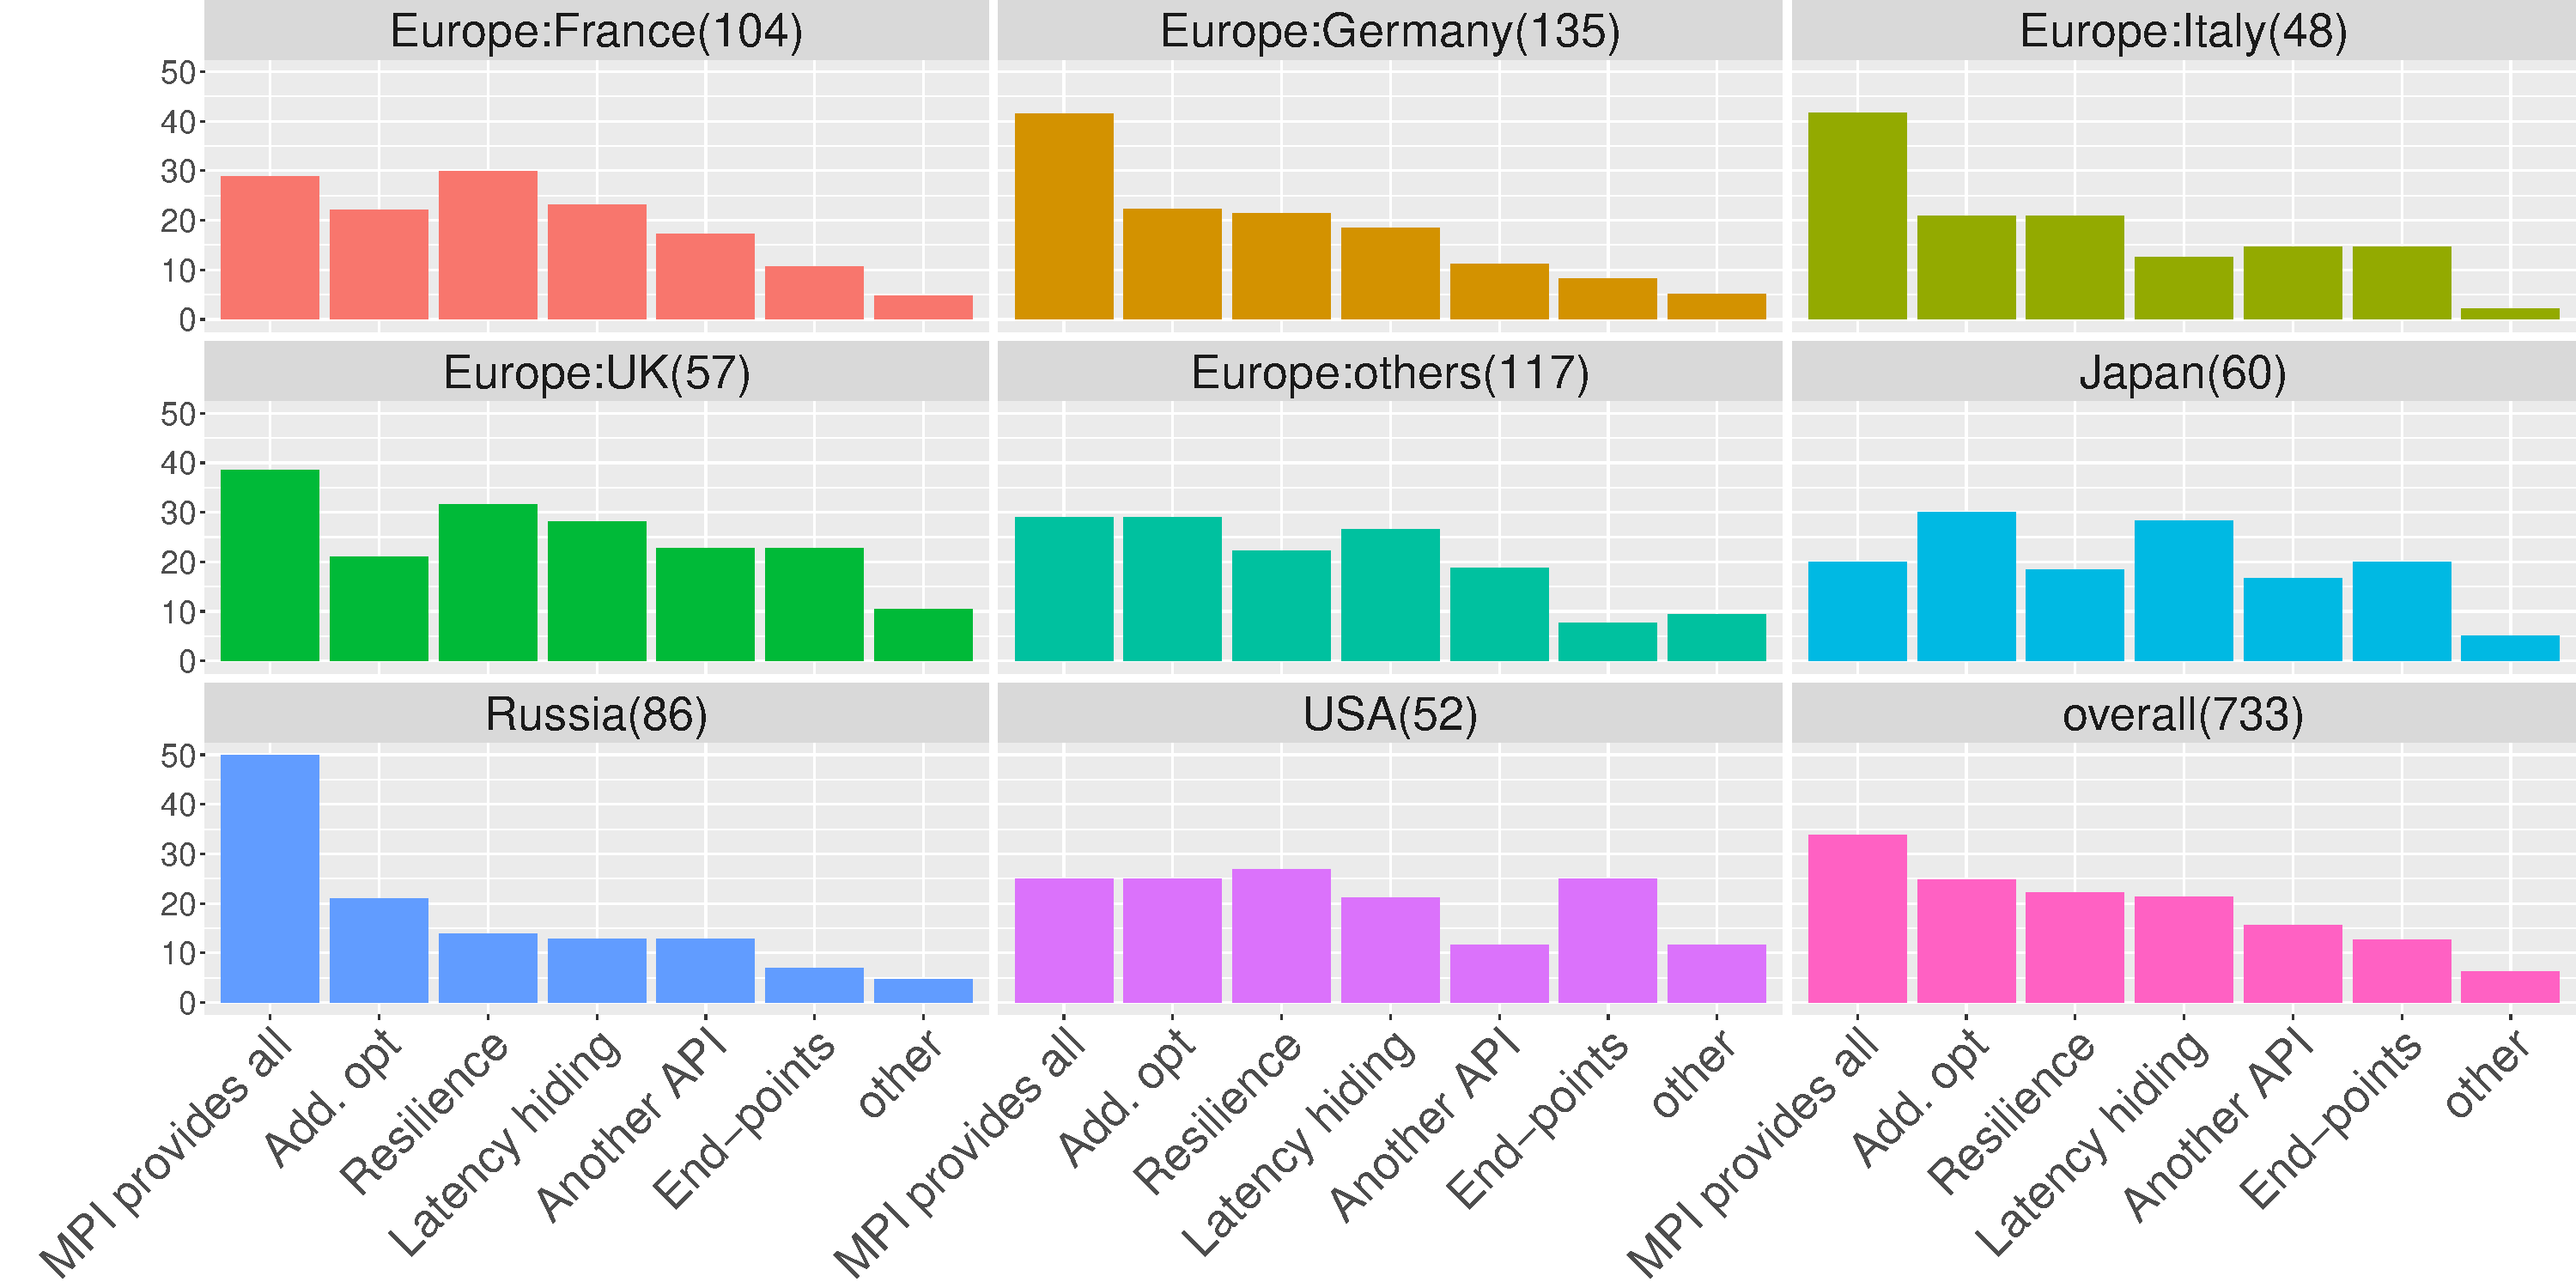
\includegraphics[width=8.0cm]{R-scripts/Q26.pdf}
\vspace{-2mm}
\caption{Q26: MPI Missing Semantics {\it(multiple)}}
\label{fig:missing-semantics}
\end{center}
\end{figure}

Finally, the least desired feature concerns the notion of endpoints, as
discussed in the MPI standardization effort. However taking into account the
extremely technical aspect of this question, and it's intricate evolution in the
standard, it might be possible that most people answering this question knew
little, and possibly imprecisely, what this feature was exactly about.

\subsection{Notes on \Countries}

In this subsection, we summarize our findings where some
\revision{\countries have}{\countries\ have} showed
somewhat different results than the others.

\subsubsection*{USA}

US has the highest percentages:
\begin{enumerate*}
\item of high MPI skill (Fig.~\ref{fig:mpi-skill})\revision{,}{;}
\item of seasoned users, with more than 10 years of MPI experience (Fig.~\ref{fig:mpi-experience})\revision{,}{;}
\item using the {\tt MULTIPLE} threading support
  (Fig.~\ref{fig:multi-thread})\revision{,}{;}
\item choosing familiar MPI implementations
  (Fig.~\ref{fig:choosing-implementation})\revision{,}{;} and
\item reading MPI books (Fig.~\ref{fig:learning-mpi})
\end{enumerate*}
among the \mcountries. All these results indicates that the MPI
users in US are, \revision{by some standards}{in a sense,} the most advanced.

\subsubsection*{Russia}

Russia is:
\begin{enumerate*}
\item having the second largest percentage of MPI users with less than 5
  years of MPI experience, a position it shared with Italy
  (Fig.~\ref{fig:mpi-experience})\revision{,}{;}
\item having the largest percentage of (non-MPI) programming beginners
  (Fig:\ref{fig:prog-skill})\revision{,}{;}
\item having the highest percentage of users assessing their MPI programs are
  well-tuned (Fig.~\ref{fig:difficulty})\revision{,}{;}
\item having the highest percentage not knowing which thread level
  they are using (Fig.~\ref{fig:multi-thread})\revision{,}{;} and
\item the second highest \country, next to US, choosing the MPI+CUDA
  (Fig.~\ref{fig:mpi-x}).
\end{enumerate*}

These findings may indicate that Russia is relatively younger in terms
of MPI usage compared with the other \mcountries. The high \revision{concern}{focus} on
MPI+CUDA, however, is very interesting.

\subsubsection*{Japan}

In this survey, Japan shows the most unique results (this is already reported
in~\cite{swopp2019}). Despite a high level of MPI skill
(Fig.~\ref{fig:mpi-skill}) and a long MPI experience
(Fig.~\ref{fig:mpi-experience}), many Japanese MPI users seem to be displeased
with the current status of debugging and tuning (Fig.~\ref{fig:difficulty}),
whilst many participants of the other \countries\ are more concerned about
\myquote{Algorithm}.

Most notably, more than 50\% of Japanese MPI users have an extensive MPI
experience, with more than 10 years. Having such a large mass of well seasoned
MPI users {\revision{sound}{sounds} promising, however, it might also point to an imbalance in
generations of users, and to a potential lack of younger MPI developers that
will continue the work in the future.
% the equally distributed answers is
% desired, thinking the continuous alternation of generations.
Indeed, the percentage of 5-to-10-year MPI experience in Japan is the smallest
among the \countries. If this lack of mid-level is true, then the
future of \revision{}{the}
Japanese HPC community might be in a difficult spot over the next decade.

\section{Discussion}

\subsection{A constantly increasing standardization document}

This survey reveals that some MPI features, which by most standards are not new\revision{}{,}
being introduced almost a decade ago, are not yet widely \revision{accepted}{adopted} by MPI users
(Subsection \ref{sec:mpi-aspects}). An interesting question may be raised
regarding the evolution of the gap between the MPI features defined by the
standard and the acceptance of the features.

\begin{figure}[tb]
\begin{center}
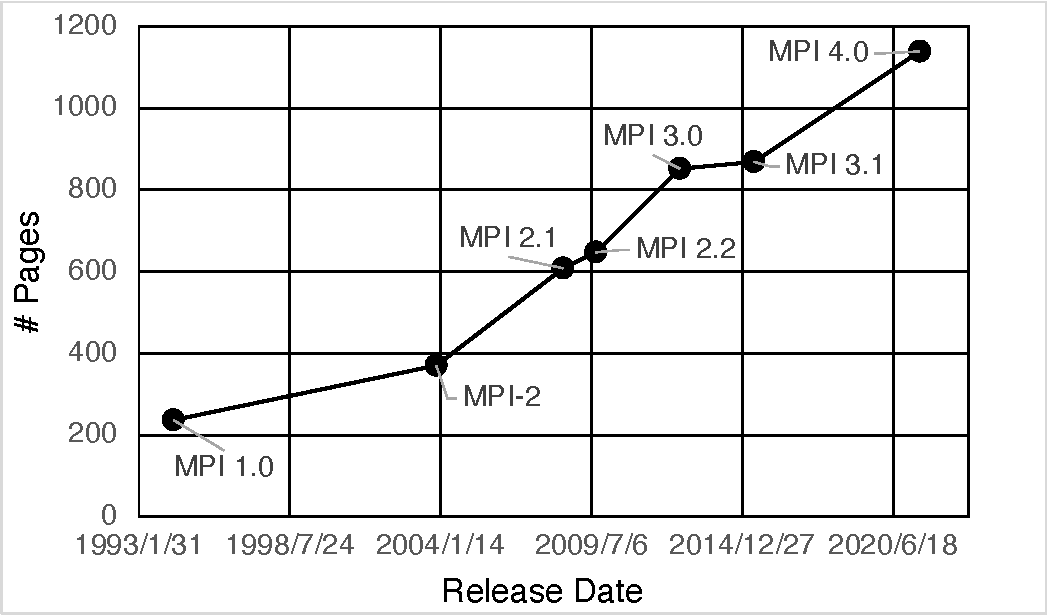
\includegraphics[width=6cm]{Figs/MPI-Standards.pdf}
\caption{Page sizes of MPI Standards}
\label{fig:mpi-standards}
\end{center}
\end{figure}

Fig.~\ref{fig:mpi-standards} shows the number of pages (in terms of PDF, not the
content) plotted over the released dates. Not surprisingly, the number of pages
increases with every new version of the standard. It is a natural thinking that
the number of pages and the number of features are proportional.

In many cases, the higher functionalities introduced by newer MPI standard yield
more degree of implementation freedom. An MPI implementation can be optimized by
exploiting hardware resources without imposing significant effort on the MPI
users. If only the most basic communication functions, send and receive, are
supported by MPI then users have to write collective functions which are not
easy if users wants optimize for the parallel machines they are using.

Another reason \revision{of}{for} the inflation is that MPI standard is the standard
as a library. There is no way for \revision{library functions to know how the
library functions are called in which context}{the implementation of low-level communication procedures
to know whether they are employed as part of a higher-level data exchange
pattern}. The higher abstracted
functions can give a library more information of \revision{how and
  which}{the higher-level information} and
thus the higher-level functions can be optimized. Tr\"{a}ff, et al., gives
a formal analysis on this point~\cite{5184825}.
This situation, introducing higher-level functions into the standard,
will keep increasing the standard.

Hoefler et al., reported their idea to extract collective operation
patterns from a series of communication primitives, send and
receive~\cite{7842939}, at run time. Applying this technique, a
communication library will be able to optimize various communication
patterns without introducing higher-level functions.
Although their idea is at the experimental
stage, however, this seems to be a good solution not introducing new
functions but narrowing the gap.

\subsection{Recommendations for MPI Forum}

Currently the MPI standard documents are available in PDF format and
hardcover books~\cite{mpi-hardcover}. There are some MPI tutorial web
sites (\cite{mpi-tutorial} as an example). \cite{mpi-tutorial-intro}
pointed out most of such web pages are out-dated and not
kept in sych with today's web standards.

As already shown in Subsection~\ref{sec:mpi-aspects}, some, rather old, MPI
features have failed to gain traction and be widely \revision{accepted}{adopted} by the users.
Furthermore, as indicated in Subsection~\ref{sec:learning-mpi}, many MPI users
complain of a lack of time to hone or master MPI, and also to a lack of clear
and easy understandable documentation. These suggest that there is a real
difficulty for people to learn MPI and to write, efficient and error-free MPI programs.

However, this can be  addresses with a stronger educational effort from the MPI
standardization body. Indeed, it is very important to narrow the gap described in
the previous subsection by helping MPI users to learn and write MPI programs. We
believe this is the responsibility of MPI Forum, since the other,
volunteer-based approach would not be efficient and sufficient. If
\revision{}{the} MPI Forum
agrees \revision{with}{on} us for narrowing the gap, then \revision{}{the} MPI Forum should
%
\begin{itemize}
    %
\item {\bf raise the bar on potential user adoption for all new features in
order to slow the pace of introducing new features,} and
%
\item {\bf create a new working group focused on educational resources, and
tasked to prepare and maintain web pages for tutorials, guidelines for MPI
programming, and good (and certainly bad) MPI examples}.
  %
\end{itemize}

\section{Summary}

We have conducted a questionnaire survey and succeeded to gather more than 850
participants from more than 40 countries and regions. By analyzing the collected
data, we have put forward few interesting findings regarding the current status
of MPI adoption. As for the MPI features, the dynamic process feature is
considered not only as a less-used feature but also mostly as a useless feature
(highlighting that the MPI programming model is seen as {\em static}). By asking
several questions how participants obtain MPI knowledge and experiences, it is
revealed that MPI is, at least perceived as\revision{}{,} a very difficult-to-use library.
\comment{Most participants read the MPI standard only partially to check the
specification of MPI functions. Instead} Many MPI users point to a lack of
documentation and would wish to have a practical programming guideline, online
documents in hyper-text form, and useful sample programs, put forward and
maintained by the MPI standardization committee. Most important (and most
difficult) thing is those supplemental documents in any form must be up-to-dated
and thorough. Regarding backward compatibility, many MPI users may accept to
sacrifice some level of portability in exchange for more performance, an outcome
at odds with the current thinking in the MPI Forum.

All collected answers, the programs to analyze the survey data and to
generate graphs, and all published reports are freely available at
{\tt \url{https://github.com/bosilca/MPIsurvey.git}}.

\section*{Acknowledgments}

We thank to those who participated in this survey and those who helped us to
distribute the questionnaire to their local communities. We especially thank to
MPI Forum members who gave us many significant comments on the draft
questionnaire. This research is partially supported by the
NCSA-Inria-ANL-BSC-JSC-Riken-UTK Joint-Laboratory for Extreme Scale
Computing~\cite{JLESC}, with additional funding from different natioanl science
agencies.

\bibliography{ref}

{\footnotesize
  \begin{description}
  \item[{[dataset][19]}] A. Hori, T. Ogura, E. Jeannot,
G. Bosilca, MPI International Survey – GitHub Repository,
\url{https://github.com/bosilca/MPIsurvey.git}, 2021.
  \end{description}
}

\appendix
\section{List of Questions and Choices}
\label{app:questions}

The followings are the list of all questions associated with
choices. The question numbers suffixed by asterisks (*) are
multiple-choice questions. The choices are followed by corresponding
abbreviations in square brackets, if any.
\vspace{2mm}
{\footnotesize
  \begin{description}
  \item[Q1:] What is your main occupation
    \begin{inparaenum}[{\bf C}1)]
    \item College/University [Univ]
    \item Governmental institute [Gov]
    \item Hardware vendor [HW]
    \item Software vendor [SW]
    \item Private research institute [priv]
    \item Other
    \end{inparaenum}
  \item[Country:] \hspace{3mm}Select main country or region of your workplace in past 5 years.
    Choose one from the country list.
  \item[Q2:] Rate your overall programming skill (non-MPI programs).
    Choose one in the range of 1 to 6. [Low-High]
  \item[Q3:] Rate your MPI programming skill.
    Choose one in the range of 1 to 6. [Low-High]
  \item[Q4*:] What programming language(s) do you use most often?
    \begin{inparaenum}[{\bf C}1)]
    \item C/C++ [C(++)]
    \item Fortran 90 or newer [\textgreater=F90]
    \item Fortran (older one than Fortran 90) [\textless F90]
    \item Python [Py]
    \item Java [Java]
    \item Other
    \end{inparaenum}
  \item[Q5:] How long have you been writing computer programs (incl. non-MPI programs)?
    \begin{inparaenum}[{\bf C}1)]
    \item more than 10 years [\textgreater10]
    \item between 5 and 10 years [5-10]
    \item between 2 and 5 years [2-5]
    \item less than 2 years [\textless 2]
    \end{inparaenum}
  \item[Q6:] How long have you been writing MPI programs?
    \begin{inparaenum}[{\bf C}1)]
    \item more than 10 years [\textgreater10]
    \item between 5 and 10 years [5-10]
    \item between 2 and 5 years [2-5]
    \item less than 2 years [\textless 2]
    \end{inparaenum}
  \item[Q7*:] Which fields are you mostly working in?
    \begin{inparaenum}[{\bf C}1)]
    \item System software development (OS, runtime library, communication
      library, etc.) [OS/R]
    \item Parallel language (incl. domain specific language) [Lang]
    \item Numerical application and/or library [Num-App/Lib]
    \item AI (Deep Learning) [AI]
    \item Image processing [Image Proc]
    \item Big data [Bg Data]
    \item Workflow and/or In-situ [Workfflow]
    \item Visualization [Visualization]
    \item Tool development (performance tuning, debugging, etc.) [Tool]
    \item Other
    \end{inparaenum}
  \item[Q8*:] What is your major role at your place of work?
    \begin{inparaenum}[{\bf C}1)]
    \item Research and development of application(s) [Apps]
    \item Research and development software tool(s) [Tools]
    \item Parallelization of sequential program(s) [parallelize]
    \item Performance tuning of MPI program(s) [Tuning]
    \item Debugging MPI programs [Debug]
    \item Research and development on system software (OS and/or runtime
      library) [OS/R]
    \item Other
    \end{inparaenum}
  \item[Q9:] Have you ever read the MPI standard specification document?
    \begin{inparaenum}[{\bf C}1)]
    \item I read all. [All]
    \item I read most of it. [Mostly]
    \item I read only the chapters of interest for my work. [Partly]
    \item I have not read it, but I plan to. [Wish]
    \item No, and I will not read it. [No]
    \end{inparaenum}
  \item[Q10*:] How did you learn MPI?
    \begin{inparaenum}[{\bf C}1)]
    \item I read the MPI standard document. [Standard]
    \item I had lecture(s) at school. [School]
    \item I read articles found on Internet. [Internet]
    \item I read book(s). [Books]
    \item Other lectures or tutorials (workplace, conference). [Other lec.]
    \item I have not learned MPI. [Never learned]
    \item Other
    \end{inparaenum}
  \item[Q11*:] Which MPI book(s) have you read?
    \begin{inparaenum}[{\bf C}1)]
    \item Beginning MPI (An Introduction in C) [Beginning MPI]
    \item Parallel Programming with MPI [Parallel Programming]
    \item Using MPI [Using MPI]
    \item Parallel Programming in C with MPI and OpenMP [Parallel
      Programming in C]
    \item MPI: The Complete Reference [MPI: Complete Ref]
    \item I have never read any MPI books [(no book)]
    \item Other
    \end{inparaenum}
  \item[Q12*:] Which MPI implementations do you use?
    \begin{inparaenum}[{\bf C}1)]
    \item MPICH
    \item Open MPI [OMPI]
    \item Intel MPI [Intel]
    \item MVAPICH [MVA]
    \item Cray MPI [Cray]
    \item IBM MPI (BG/Q, PE, Spectrum) [IBM]
    \item HPE MPI [HPE]
    \item Tianhe MPI [Tianhe]
    \item Sunway MPI [Sunway]
    \item Fujitsu MPI [Fujitsu]
    \item NEC MPI [NEC]
    \item MS MPI [MS]
    \item MPC MPI [MPC]
    \item I do not know [No idea]
    \item Other
    \end{inparaenum}
  \item[Q13:] Why did you choose the MPI implementation(s)?
    \begin{inparaenum}[{\bf C}1)]
    \item I like to use it. [I like]
    \item I was said to use it. [Said to use]
    \item I could not have any choice (the one provided by a vendor). [No choice]
    \item I am familiar with it. [Familiar]
    \item I have no special reason. [No reason]
    \end{inparaenum}
  \item[Q14*:] How do you check MPI specifications when you are writing MPI programs?
    \begin{inparaenum}[{\bf C}1)]
    \item I read the MPI Standard document (web/book). [MPI standard]
    \item I read online documents (such as man pages). [Online docs]
    \item I search the Internet (Google / Stack Overflow). [Internet]
    \item I ask colleagues. [Colleagues]
    \item I read book(s) (except the MPI standard). [Books]
    \item I know almost all MPI routines. [I know all]
    \item Other
    \end{inparaenum}
  \item[Q15:] What is the most difficult part of writing an MPI program?
    \begin{inparaenum}[{\bf C}1)]
    \item Algorithm design [Algorithm]
    \item Debugging [Debugging]
    \item Domain decomposition [Decomposition]
    \item Finding appropriate MPI routines [Finding MPI routines]
    \item Implementation issue workaround [Workaround]
    \item Performance tuning [Tuning]
    \item Other
    \end{inparaenum}
  \item[Q16*:] Which MPI features have you never heard of?
    \begin{inparaenum}[{\bf C}1)]
    \item Point-to-point communications [Point-to-point]
    \item Collective communications [Collectives]
    \item Communicator operations (split, duplicate, and so on) [Communicator]
    \item MPI datatypes [Datatypes]
    \item One-sided communications [One-sided]
    \item Dynamic process creation [Dyn. process]
    \item Persistent communication [Persistent]
    \item PMPI interface [PMPI]
    \item MPI with OpenMP (or multithread) [with OpenMP]
    \item Other
    \end{inparaenum}
  \item[Q17*:] What aspects of the MPI standard do you use in your program in its current form?
    \begin{inparaenum}[{\bf C}1)]
    \item Point-to-point communications [Point-to-point]
    \item Collective communications [Collectives]
    \item Communicator operations (split, duplicate, and so on) [Communicator]
    \item MPI datatypes [Datatypes]
    \item One-sided communications [One-sides]
    \item Dynamic process creation [Dyn. process]
    \item Persistent communications [Persistent]
    \item MPI with OpenMP (or multithread) [with OpenMP]
    \item PMPI interface [PMPI]
    \item Other
    \end{inparaenum}
  \item[Q18*:] Which MPI thread support are you using?
    \begin{inparaenum}[{\bf C}1)]
    \item MPI\_THREAD\_SINGLE [SINGLE]
    \item MPI\_THREAD\_FUNNELED [FUNNELED]
    \item MPI\_THREAD\_SERIALIZED [SERIALIZED]
    \item MPI\_THREAD\_MULTIPLE [MULTIPLE]
    \item I have never called {\tt MPI\_INIT\_THREAD} [never used]
    \item I do not know or I do not care. [No idea]
    \item Other
    \end{inparaenum}
  \item[Q19*:] What are your obstacles to mastering MPI?
    \begin{inparaenum}[{\bf C}1)]
    \item I have no obstacles. [No obstacles]
    \item Too many routines. [Too many routines]
    \item No appropriate lecture / book / info. [No appropriate one]
    \item Too complicated and hard to understand. [Complicated]
    \item I have nobody to ask. [Nobody to ask]
    \item I do not like the API. [Dislike API]
    \item Other
    \end{inparaenum}
  \item[Q20:] When you call an MPI routine, how often do you check the error code of the MPI routine  (excepting MPI-IO)?
    \begin{inparaenum}[{\bf C}1)]
    \item I rely on the default ‘Errors abort’ error handling [Default]
    \item Always
    \item Mostly
    \item Sometimes
    \item Never
    \item Other
    \end{inparaenum}
  \item[Q21:] In most of your programs, do you pack MPI function calls into their own file or files to have your own abstraction layer for communication?
    \begin{inparaenum}[{\bf C}1)]
    \item Yes, to minimize the changes of communication API. [Yes]
    \item Yes, but I have no special reason for doing that. [Yes, but no reason]
    \item No, my program is too small to do that. [No, too small]
    \item No, MPI calls are scattered in my programs. [No, scattered]
    \item Other
    \end{inparaenum}
  \item[Q22*:] Have you ever written MPI+”X” programs?
    \begin{inparaenum}[{\bf C}1)]
    \item OpenMP [OMP]
    \item Pthread
    \item OpenACC [OACC]
    \item OpenCL [OCL]
    \item CUDA
    \item No
    \item Other
    \end{inparaenum}
  \item[Q23:] Is there any room for performance tuning in your MPI programs?
    \begin{inparaenum}[{\bf C}1)]
    \item No, my MPI programs are well-tuned. [Well-tuned]
    \item Yes, I know there is room for tuning but I should re-write large
      part of my program to do that. [Hard to rewrite]
    \item Yes, I know there is room for tuning but I do not have enough resources to do that.
      [No resource]
    \item I think there is room but I do not know how to tune it.
      [No idea to tune]
    \item I do not have (know) tools to find performance bottlenecks.
      [Not having the tools]
    \item I have no chance to investigate.
      [No chance to investigate]
    \item I do not know how to find bottlenecks.
      [No idea to find bottlenecks]
    \item I do not know if there is room for performance tuning.
      [No idea to improve]
    \item Other
    \end{inparaenum}
  \item[Q24*:] What, if any, alternatives are you investigating to
    indirectly call MPI or another communication layer by using another
    parallel language/library?
    \begin{inparaenum}[{\bf C}1)]
    \item A framework or library using MPI. [Framework]
    \item A PGAS language (UPC, Coarray Fortran, OpenSHMEM, XcalableMP,
      ...). [PGAS]
    \item A Domain Specific Language (DSL). [DSL]
    \item Low-level communication layer provided by vendor (Verbs, DCMF,
      ...). [LL comm]
    \item I am not investigating any alternatives. [No investigation]
    \item Other
    \end{inparaenum}
  \item[Q25:] If there were one communication aspect which is not enough
    in the current MPI could improve the performance of your application,
    what would you prioritize? Or is MPI providing all the communication
    semantics required by your application? If not, what is missing?
    \begin{inparaenum}[{\bf C}1)]
    \item Latency [Latency]
    \item Message injection rate [Injection rate]
    \item Bandwidth [Bandwidth]
    \item Additional optimization opportunities in terms of communication
      (network topology awareness, etc.) [Additional comm. opt.]
    \item Optimization opportunities except communication (architecture
      awareness, dynamic processing, accelerator support, etc.) [Other opt.]
    \item Multi-threading support [Multi-thread]
    \item Asynchronous progress [Asynch progress]
    \item MPI provides all semantics I need [Satisfied]
    \item Other
    \end{inparaenum}
  \item[Q26*:] Is MPI providing all the communication semantics required
    by your application? If not, what is missing?
    \begin{inparaenum}[{\bf C}1)]
    \item Latency hiding (including asynchronous completion) [Latency hiding]
    \item Endpoints (multi-thread, sessions) [End-points]
    \item Resilience (fault tolerance) [Resilience]
    \item Additional optimization opportunities in terms of communication
      (topology awareness, locality, etc.) [Additional opt]
    \item Another API which is easier and/or simpler to use [Another API]
    \item MPI is providing all the communication semantics required by my
      application [MPI provides all]
    \item Other
    \end{inparaenum}
  \item[Q27*:] What MPI feature(s) are NOT useful for your application?
    \begin{inparaenum}[{\bf C}1)]
    \item One-sided communication [One-sided]
    \item Datatypes [Datatypes]
    \item Communicator and group management [Communicator]
    \item Collective operations [Collectives]
    \item Process topologies [Topologies]
    \item Dynamic process creation [Dyn. process]
    \item Error handlers [Error]
    \item There are no unnecessary features [No]
    \item Other
    \end{inparaenum}
  \item[Q28:] Do you think the MPI standard should maintain backward
    compatibility?
    \begin{inparaenum}[{\bf C}1)]
    \item Yes, compatibility is very important for me. [Very important]
    \item API should be clearly versioned. [Versioned API]
    \item I prefer to have new API for better performance. [New API for performance]
    \item I prefer to have new API which is simpler and/or
      easier-to-use. [New API for easier-to-use]
    \item I do not know or I do not care. [No idea]
    \item Other
    \end{inparaenum}
  \item[Q29:] In the tradeoff between code portability and performance,
    which is more or less important for you to write MPI programs?
    Choose one in the range of 1 to 6. [Portability-Performance]
  \end{description}
}

\section{\Countries}
\label{app:countries}

\begin{table}[ht]%
\begin{center}%
\caption{\Countries}
{\footnotesize
\begin{tabular}{l|c|r}%
\hline%
Country & Region Category & \# Participants \\%
\hline%
Germany & Europe:Germany & 159\\%
France & Europe:France & 125\\%
Russia &  & 94\\%
UK & Europe:UK & 67\\%
Japan & & 64\\%
USA & & 58\\%
Italy & Europe:Italy & 57\\%
Switzerland & Europe:others & 40\\%
Korea, South &  & 27\\%
Austria & Europe:others & 26\\%
China & & 16\\%
Sweden & Europe:others & 15\\%
Spain & Europe:others & 14\\%
India &  & 12\\%
Poland & Europe:others & 10\\%
Netherlands & Europe:others & 8\\%
Brazil &  & 6\\%
Denmark & Europe:others & 6\\%
Czech Republic & Europe:others & 5\\%
Luxembourg & Europe:others & 5\\%
Canada &  & 4\\%
Finland & Europe:others & 3\\%
Argentina & & 3\\%
Australia & & 3\\%
Taiwan &  & 2\\%
Serbia & Europe:others & 2\\%
Pakistan &  & 2\\%
Egypt &  & 2\\%
Greece & Europe:others & 2\\%
Belgium & Europe:others & 2\\%
Tunisia &  & 1\\%
Peru &  & 1\\%
Singapore & & 1\\%
Norway & Europe:others & 1\\%
Mexico &  & 1\\%
Denmark, Austria & Europe:others & 1\\%
Croatia & Europe:others & 1\\%
Portugal & Europe:others & 1\\%
Estonia & Europe:others & 1\\%
Saudi Arabia & & 1\\%
UAE & & 1\\%
Ukraine & Europe:others & 1\\%
\hline%
42 \countries & & 851  \\%
\hline%
\end{tabular}%
}%
\end{center}%
\end{table}%

\end{document}
